%%% Local Variables:
%%% mode: latex
%%% TeX-master: "gis18"
%%% End:
\section{Experimental Study}
\label{sec-exp}

\eat{
\begin{table*}[!ht]
	\renewcommand{\arraystretch}{1.20}
	\caption{\small Real-life Trajectory Datasets}
	\vspace{-1.5ex}
	\centering
	\footnotesize
	%\scriptsize
	\begin{tabular}{|l|c|c|c|r|}
		\hline
		\bf{ Data Sets}& \bf{Number\ of Trajectories}     &\bf {Sampling Rates\ (s)}   &\bf{Points Per Trajectory\ (K)}    &\bf {Total points} \\
		\hline
		\sercar	&1,000	    &3-5	    &$\sim114.0$   &114M\\
		\hline
		\geolife &182	    &1-5	    &$\sim131.4$   &24.2M\\
		\hline
		\mopsi &51	    	&2	    &$\sim153.9$     &7.9M\\
		\hline
	\end{tabular}
	\label{tab:datasets}
	\vspace{-2ex}
\end{table*}
}

\begin{table}[tb!]
	\renewcommand{\arraystretch}{1.20}
	\caption{\small Real-life Trajectory Datasets}
	\vspace{-1.5ex}
	\centering
	\footnotesize
	%\scriptsize
	\begin{tabular}{|l|c|c|r|}
		\hline
		\bf{ Properties of Data Sets} & \sercar      &\geolife   &\mopsi \\
		\hline
		{Number\ of Trajectories}	&1,000	    &182	    & 51  \\
		\hline
		 {Sampling Rates\ (s)} &3-5  & 1-5 & 2 \\
		\hline
		{Points Per Trajectory\ (K)}  &	$\sim114.0$    &$\sim131.4$	    & $\sim153.9$ \\
		\hline
		 {Total points (M)} &114   	    	&24.2    &7.9\\
		\hline
	\end{tabular}
	\label{tab:datasets}
	\vspace{-2ex}
\end{table}


In this section, we present an extensive experimental study of our one-pass trajectory tracking algorithms (\citt, \sitt and \bitt) compared with the
existing algorithms of \ldrh and \grts on trajectory datasets. Using three real-life trajectory datasets, we conducted sets of experiments to evaluate:
(1) the compression ratios,
(2) the number of messages (including data points and velocities),
(3) the max and average errors, and
(4) the running time of algorithms \citt, \sitt and \bitt vs. \ldrh and \grts. 
Among them, the impacts of error bounds and distance metrics on messages, errors and running time of these algorithms are evaluated. 




\begin{figure*}[tb!]
	\centering
	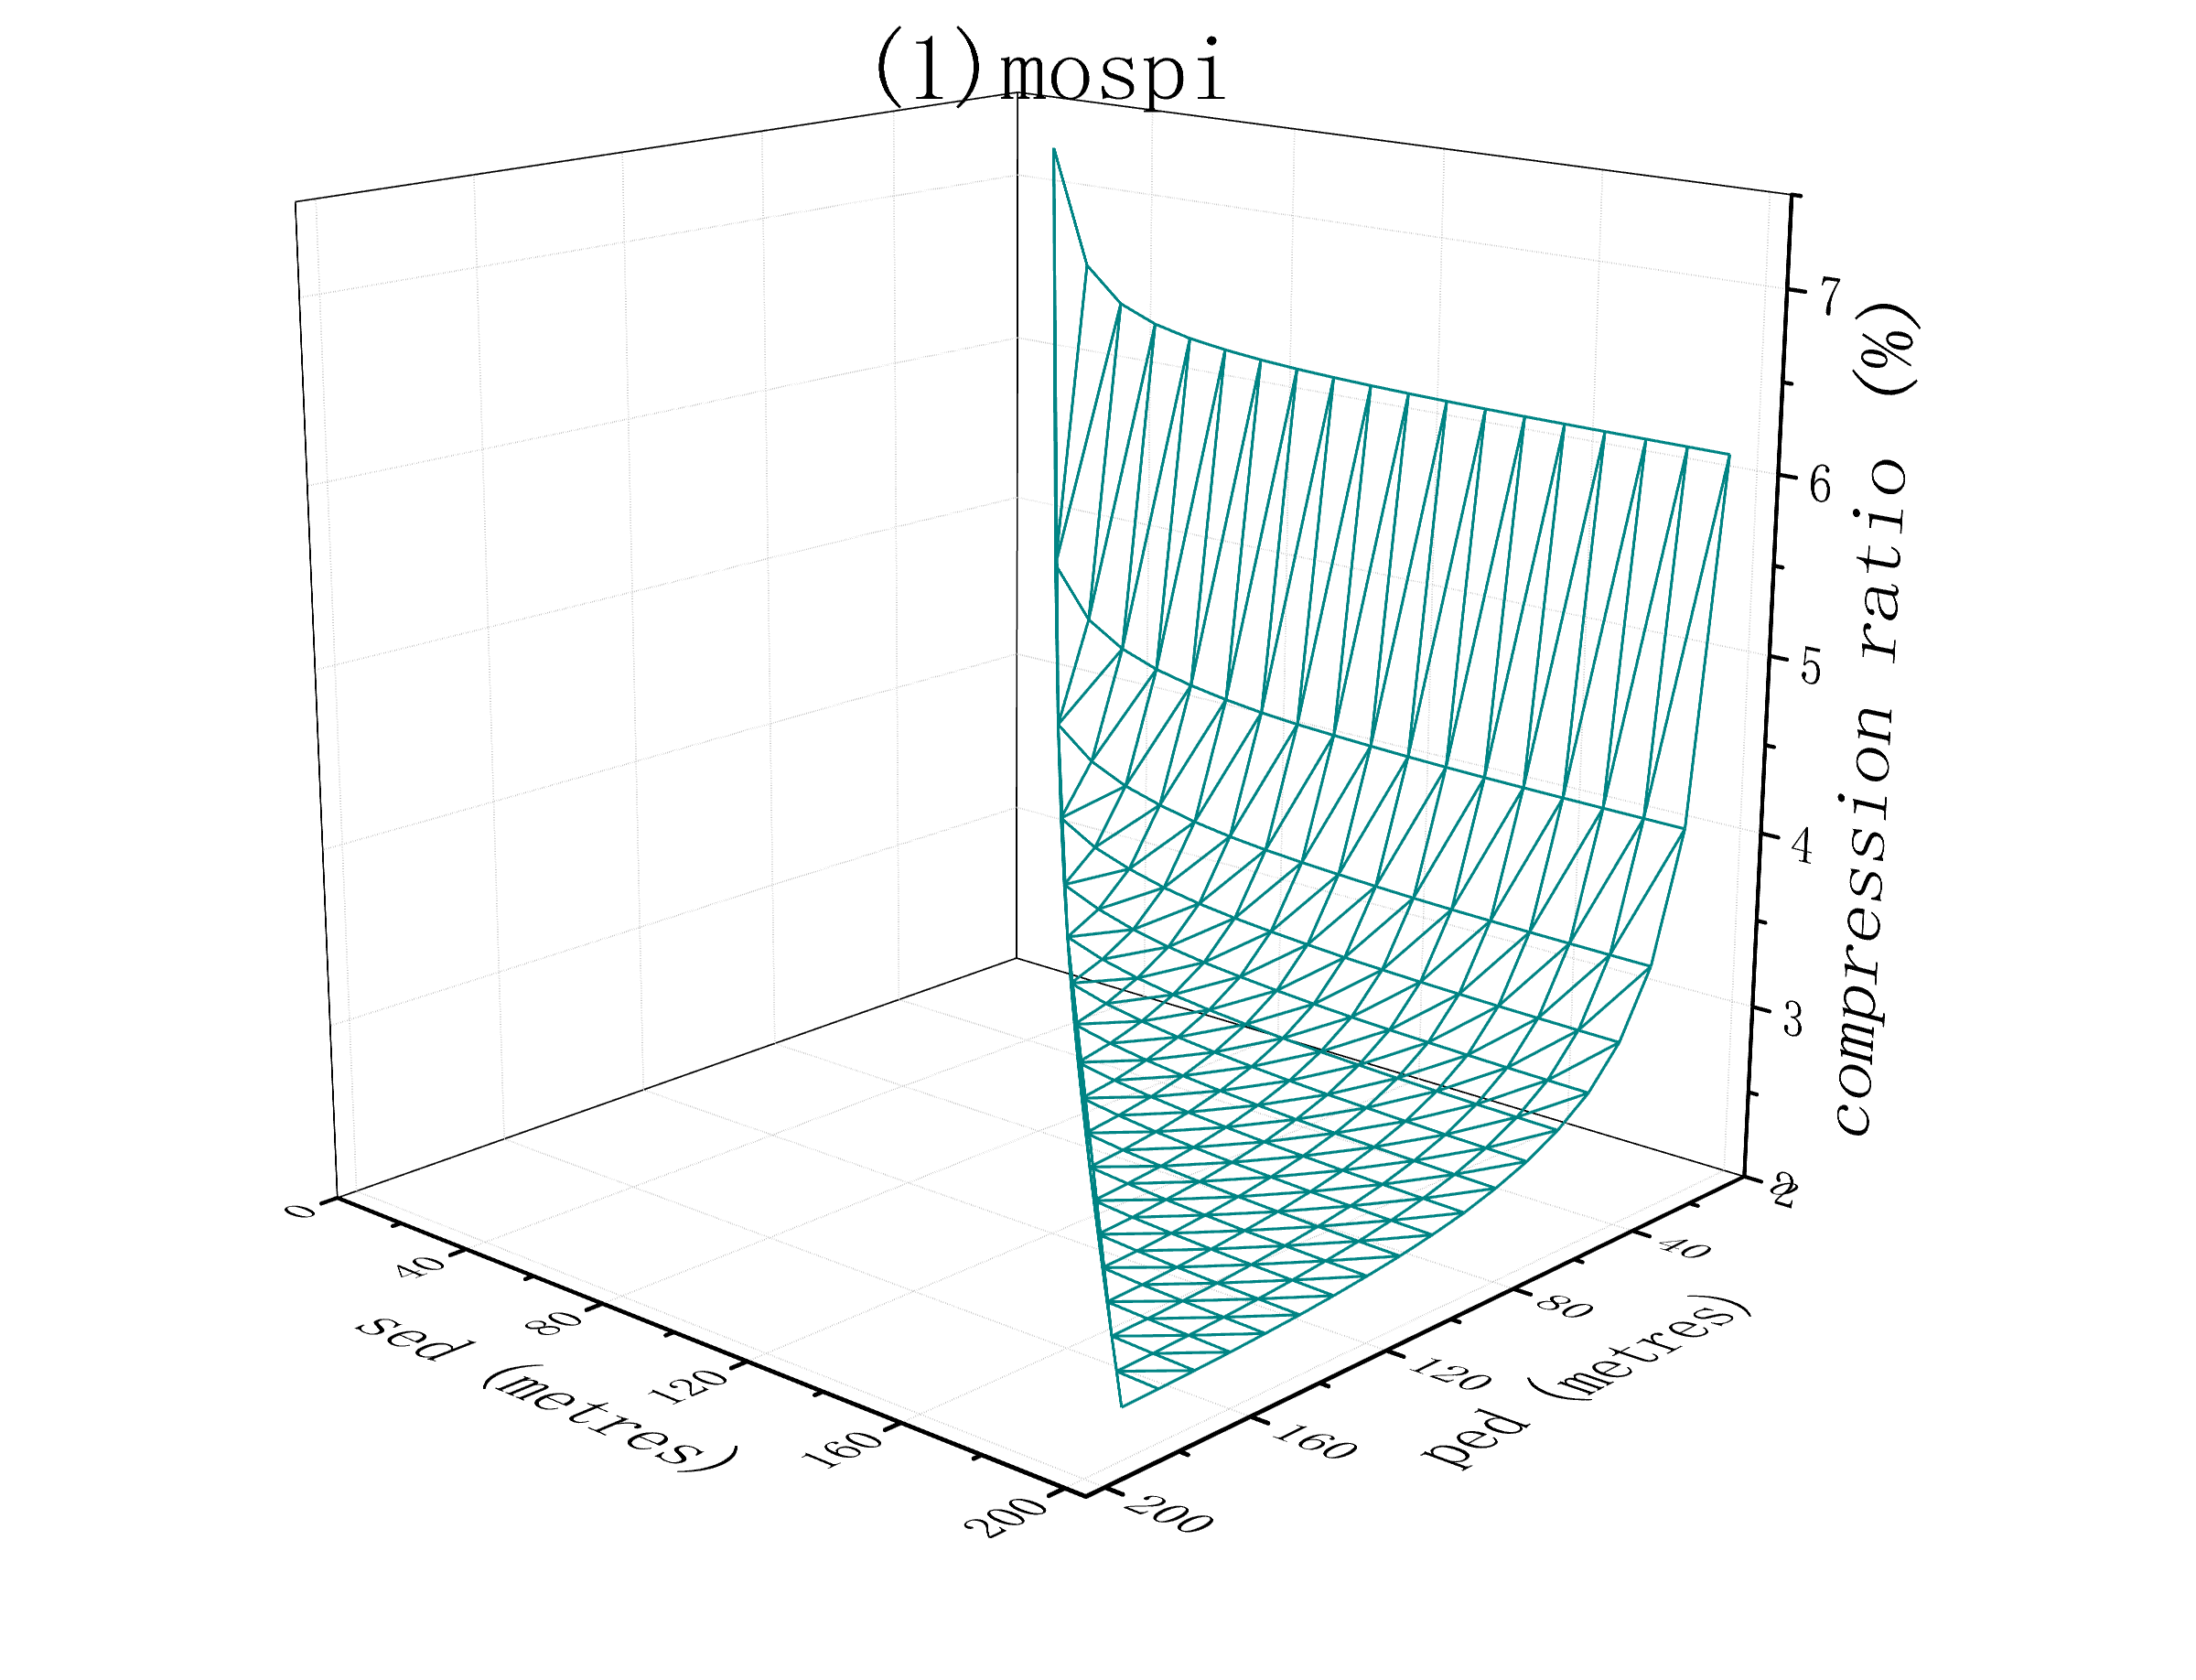
\includegraphics[scale = 0.56]{figures/Fig-BITT-mopsi-compression-ratio.png}\hspace{1ex}
	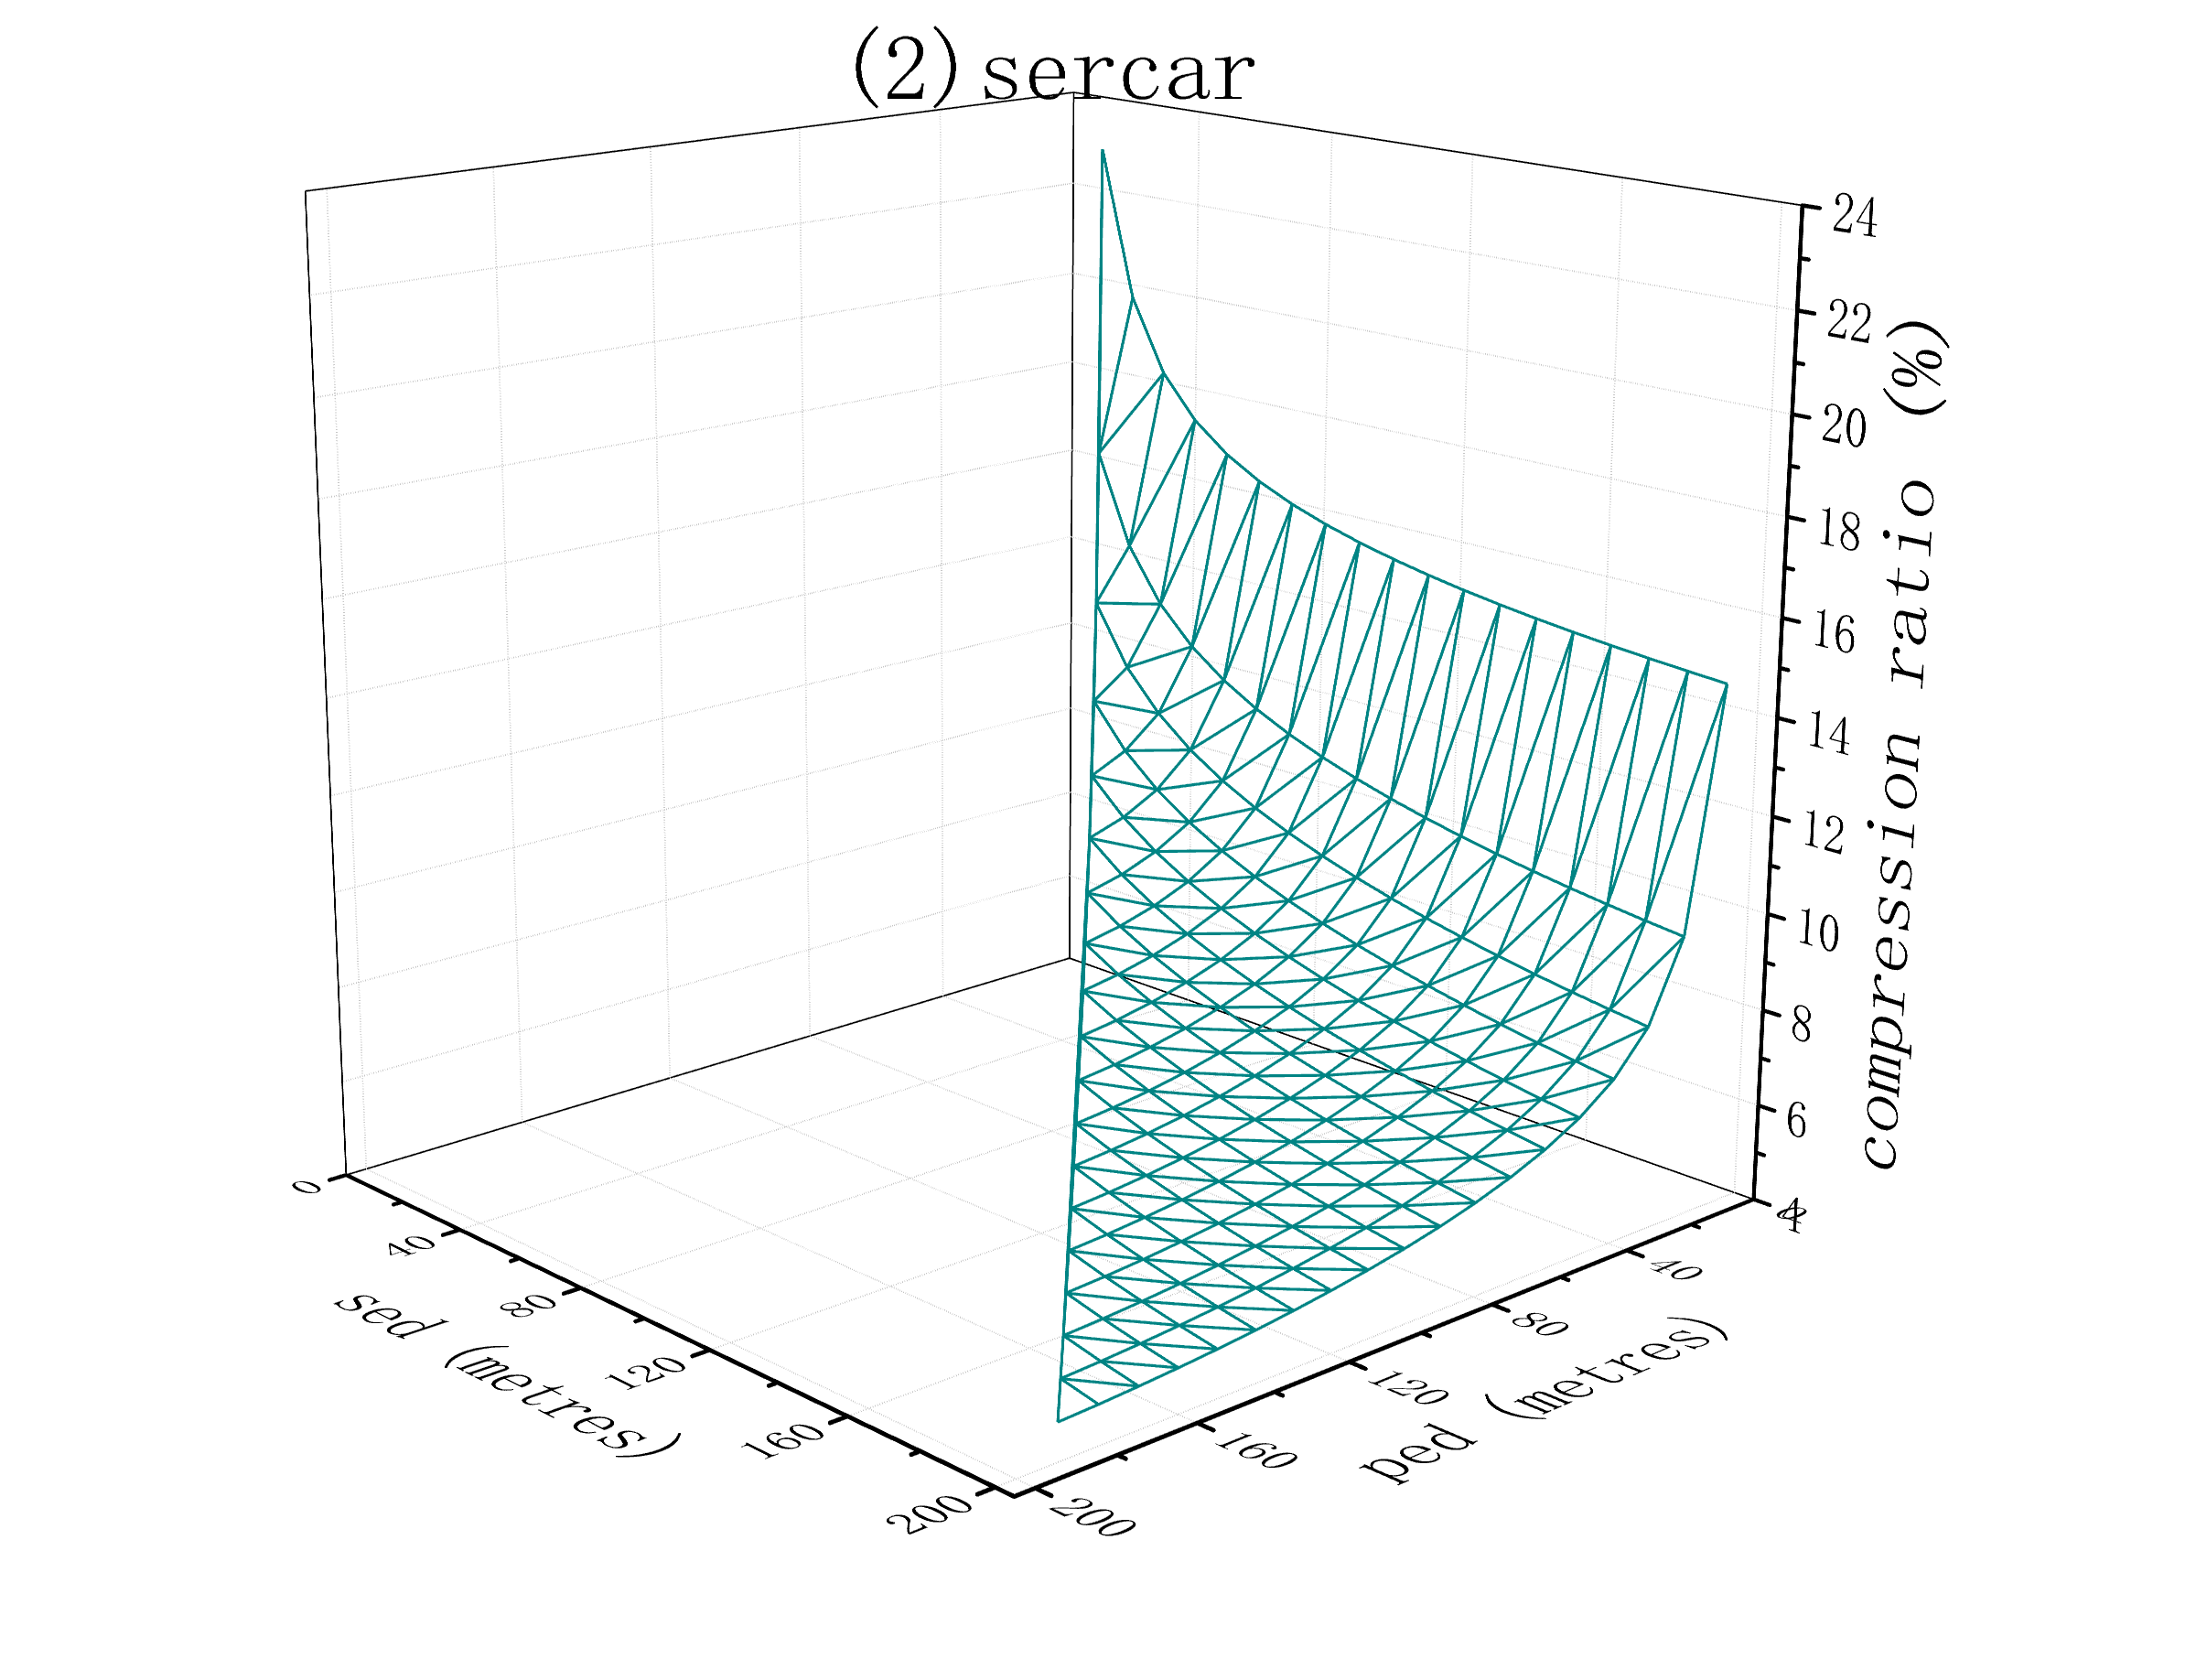
\includegraphics[scale = 0.56]{figures/Fig-BITT-sercar-compression-ratio.png}\hspace{1ex}
	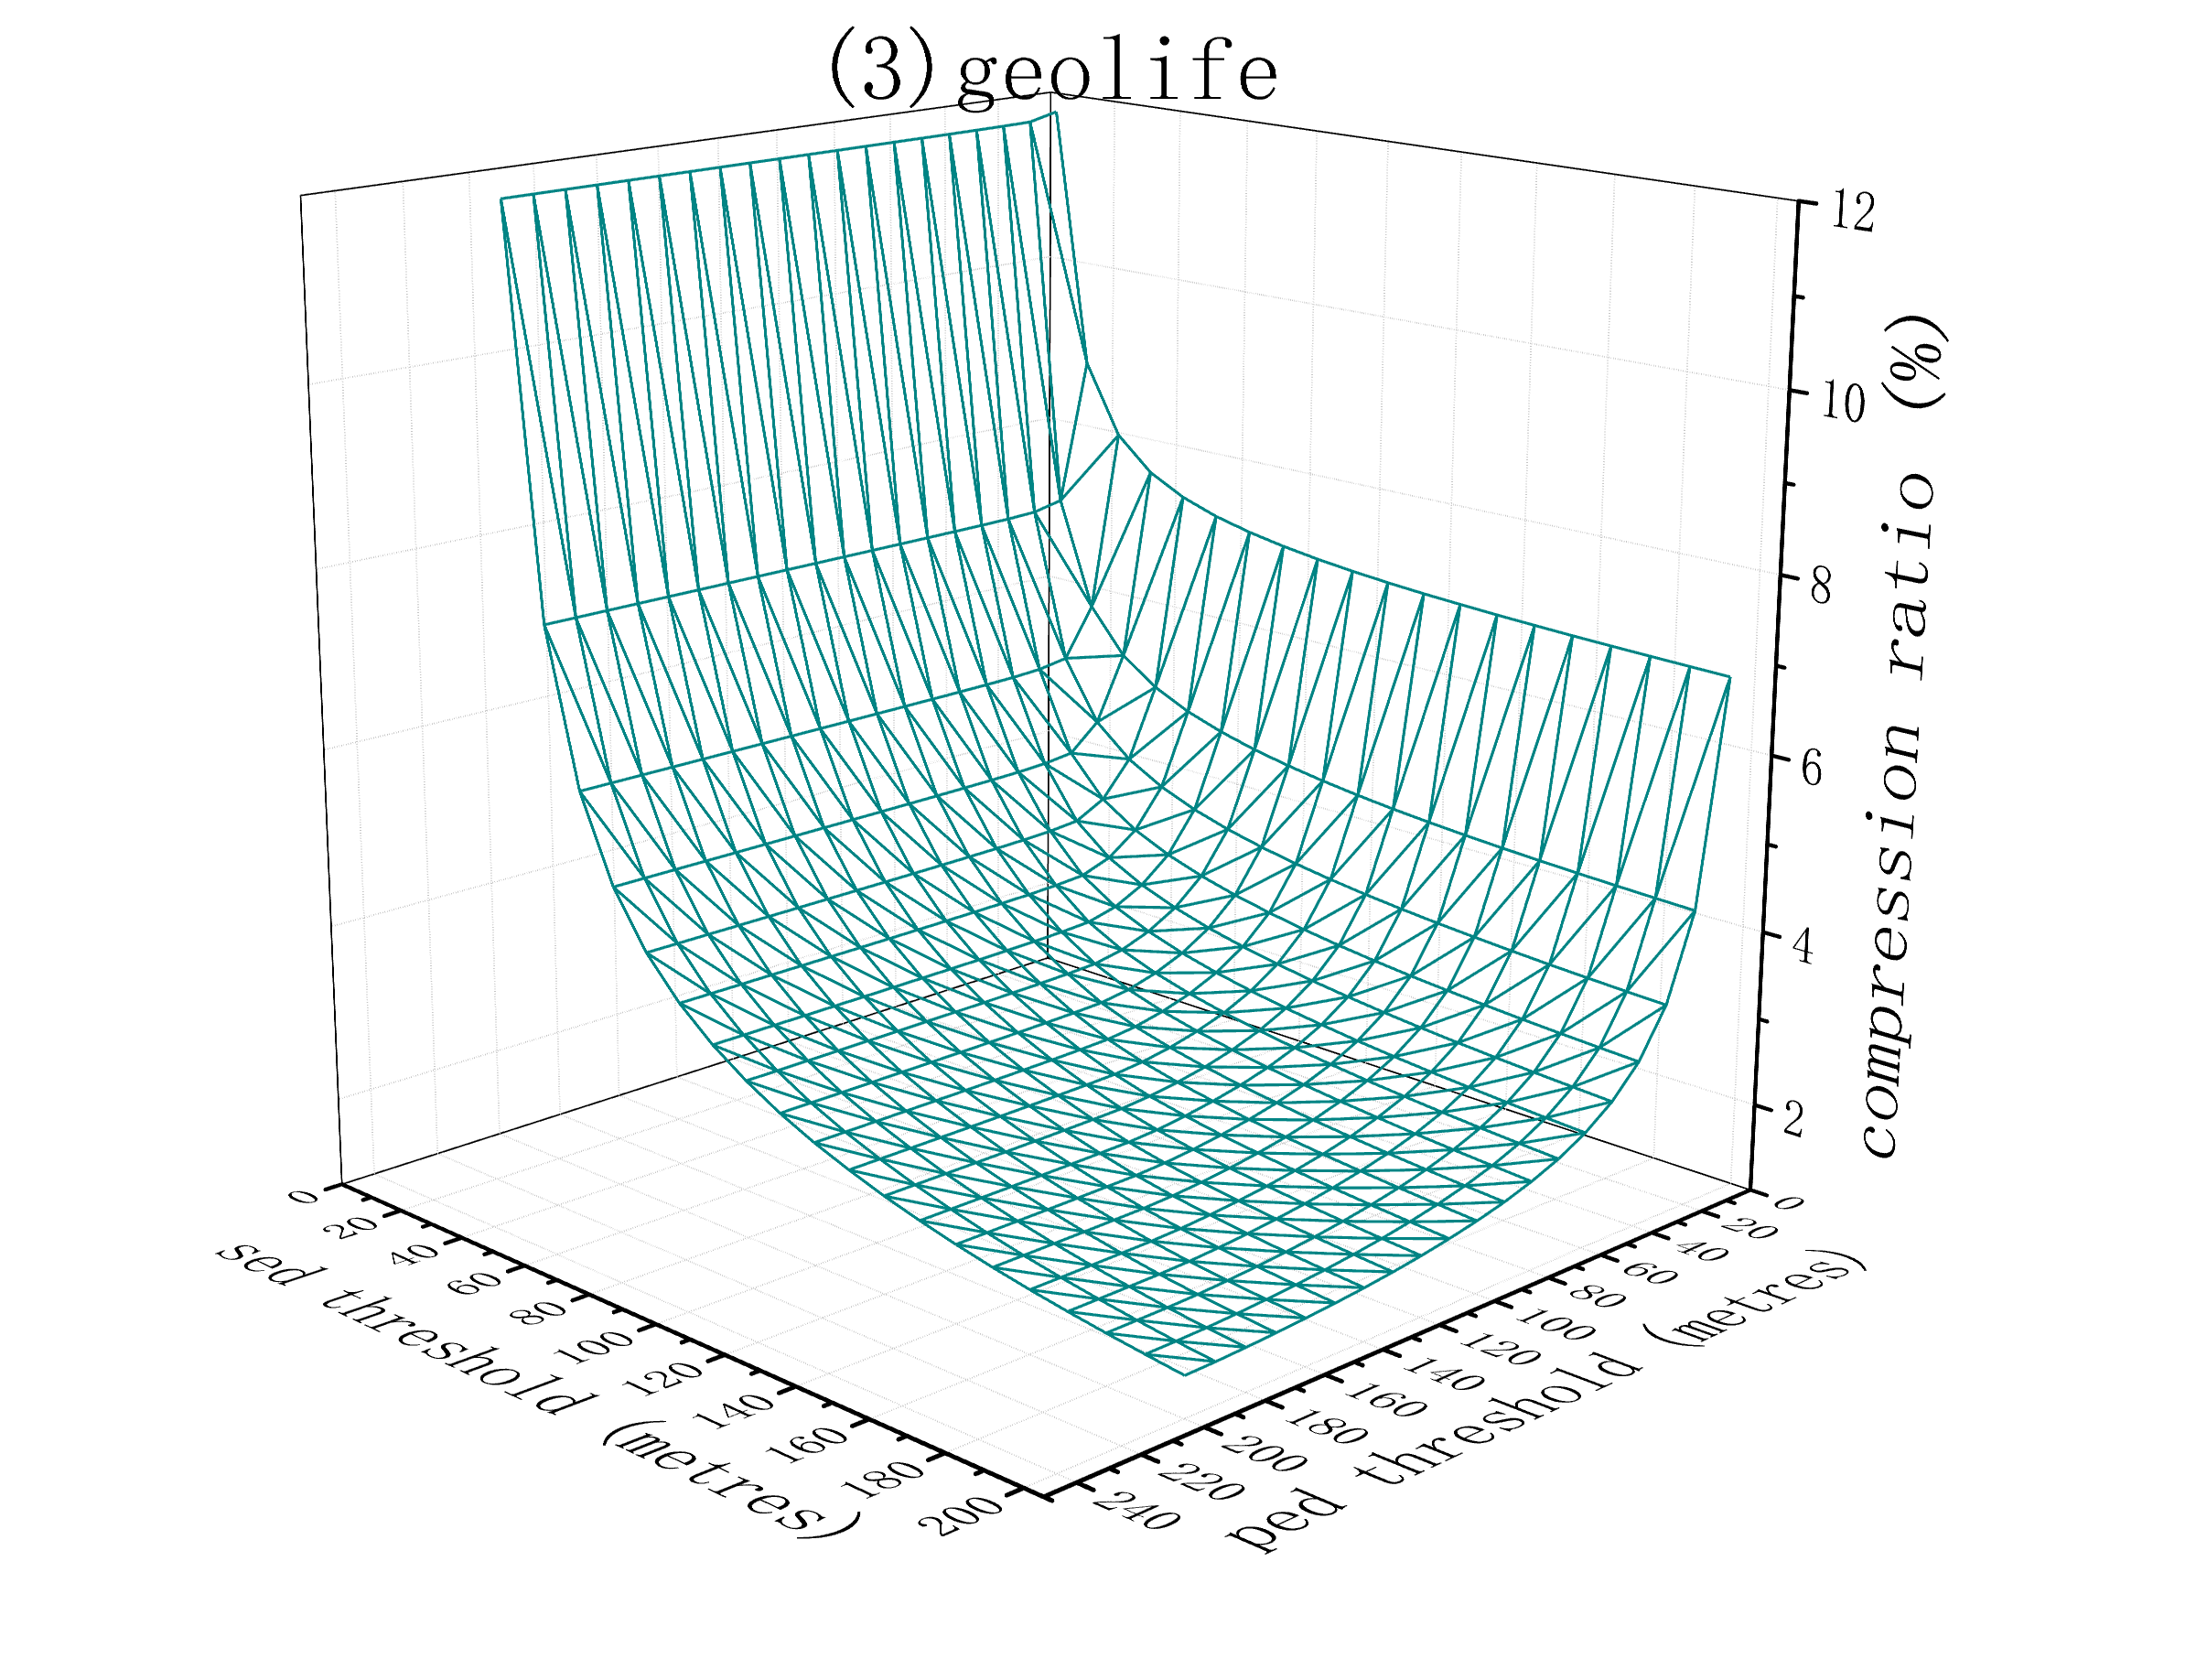
\includegraphics[scale = 0.56]{figures/Fig-BITT-geolife-compression-ratio.png}\hspace{1ex}
	\vspace{-2ex}
	\caption{\small Evaluation of the compression ratios of \bitt: varying error bounds $\epsilon_{sed}$ and $\epsilon_{ped}$.}
	\label{fig:bitt-compression-ratio}
	\vspace{-1ex}
\end{figure*}


\begin{figure*}[tb!]
	\centering
	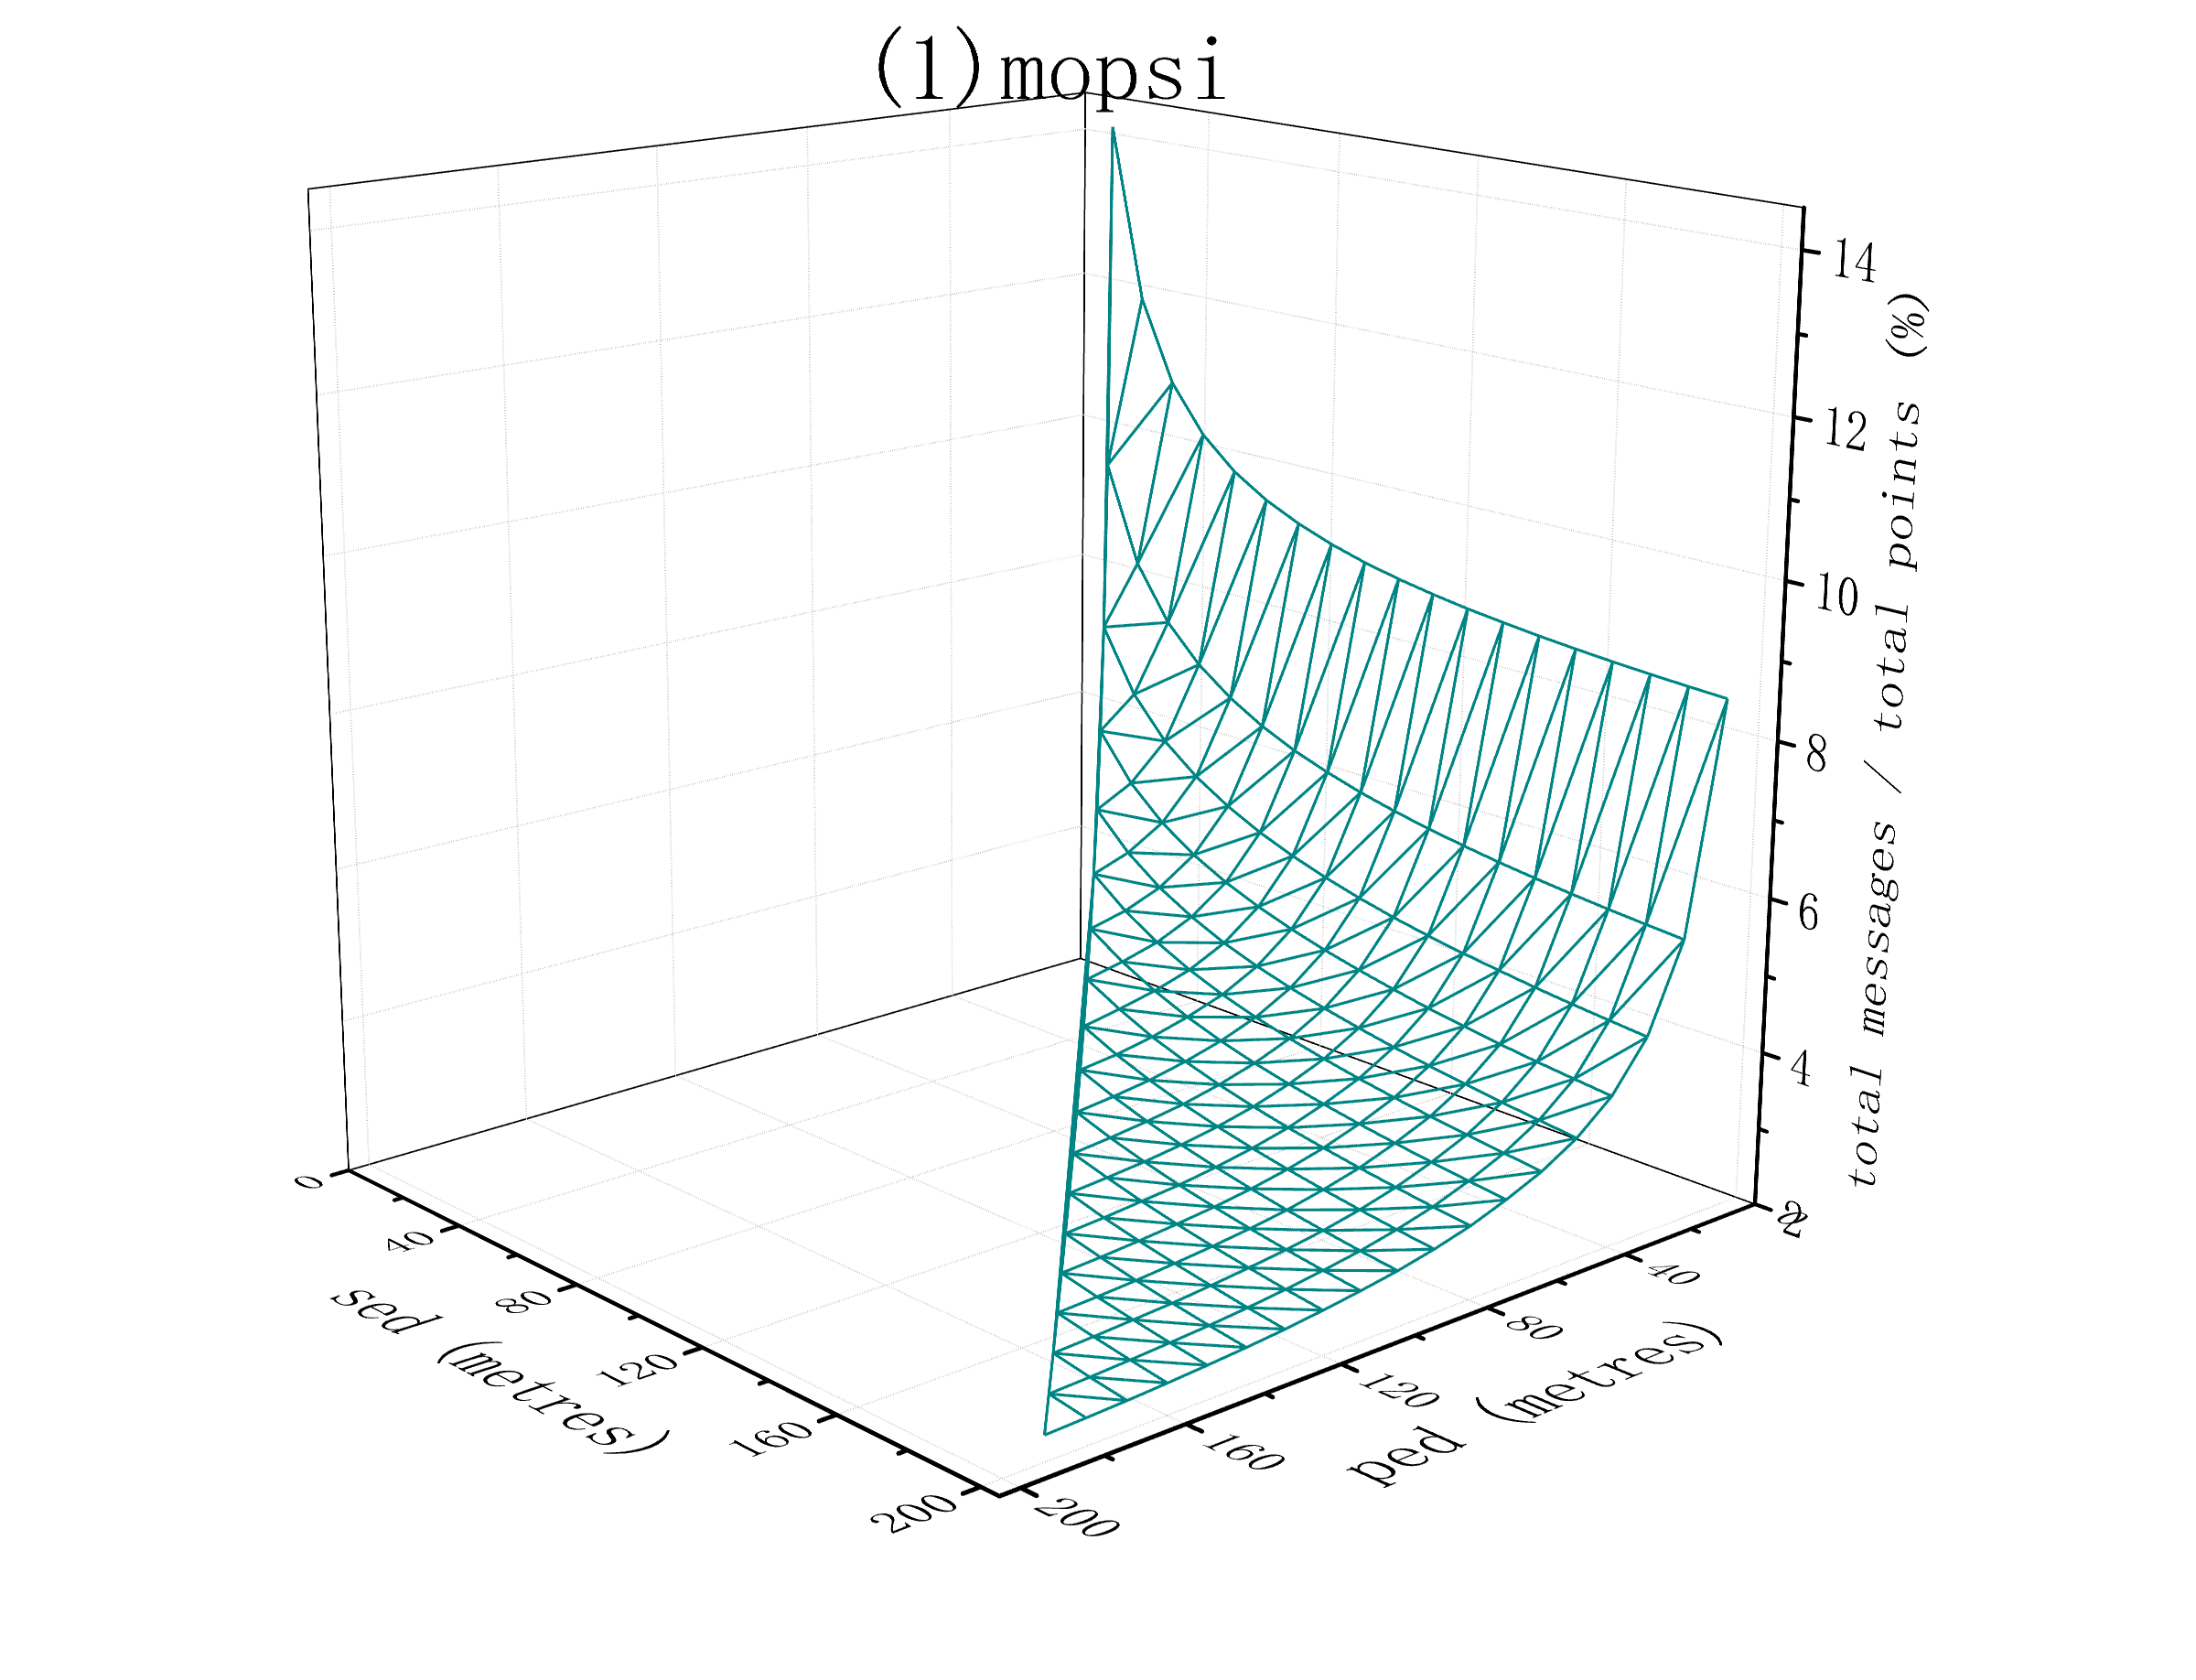
\includegraphics[scale = 0.565]{figures/Fig-BITT-mopsi-total-messages.png}\hspace{1ex}
	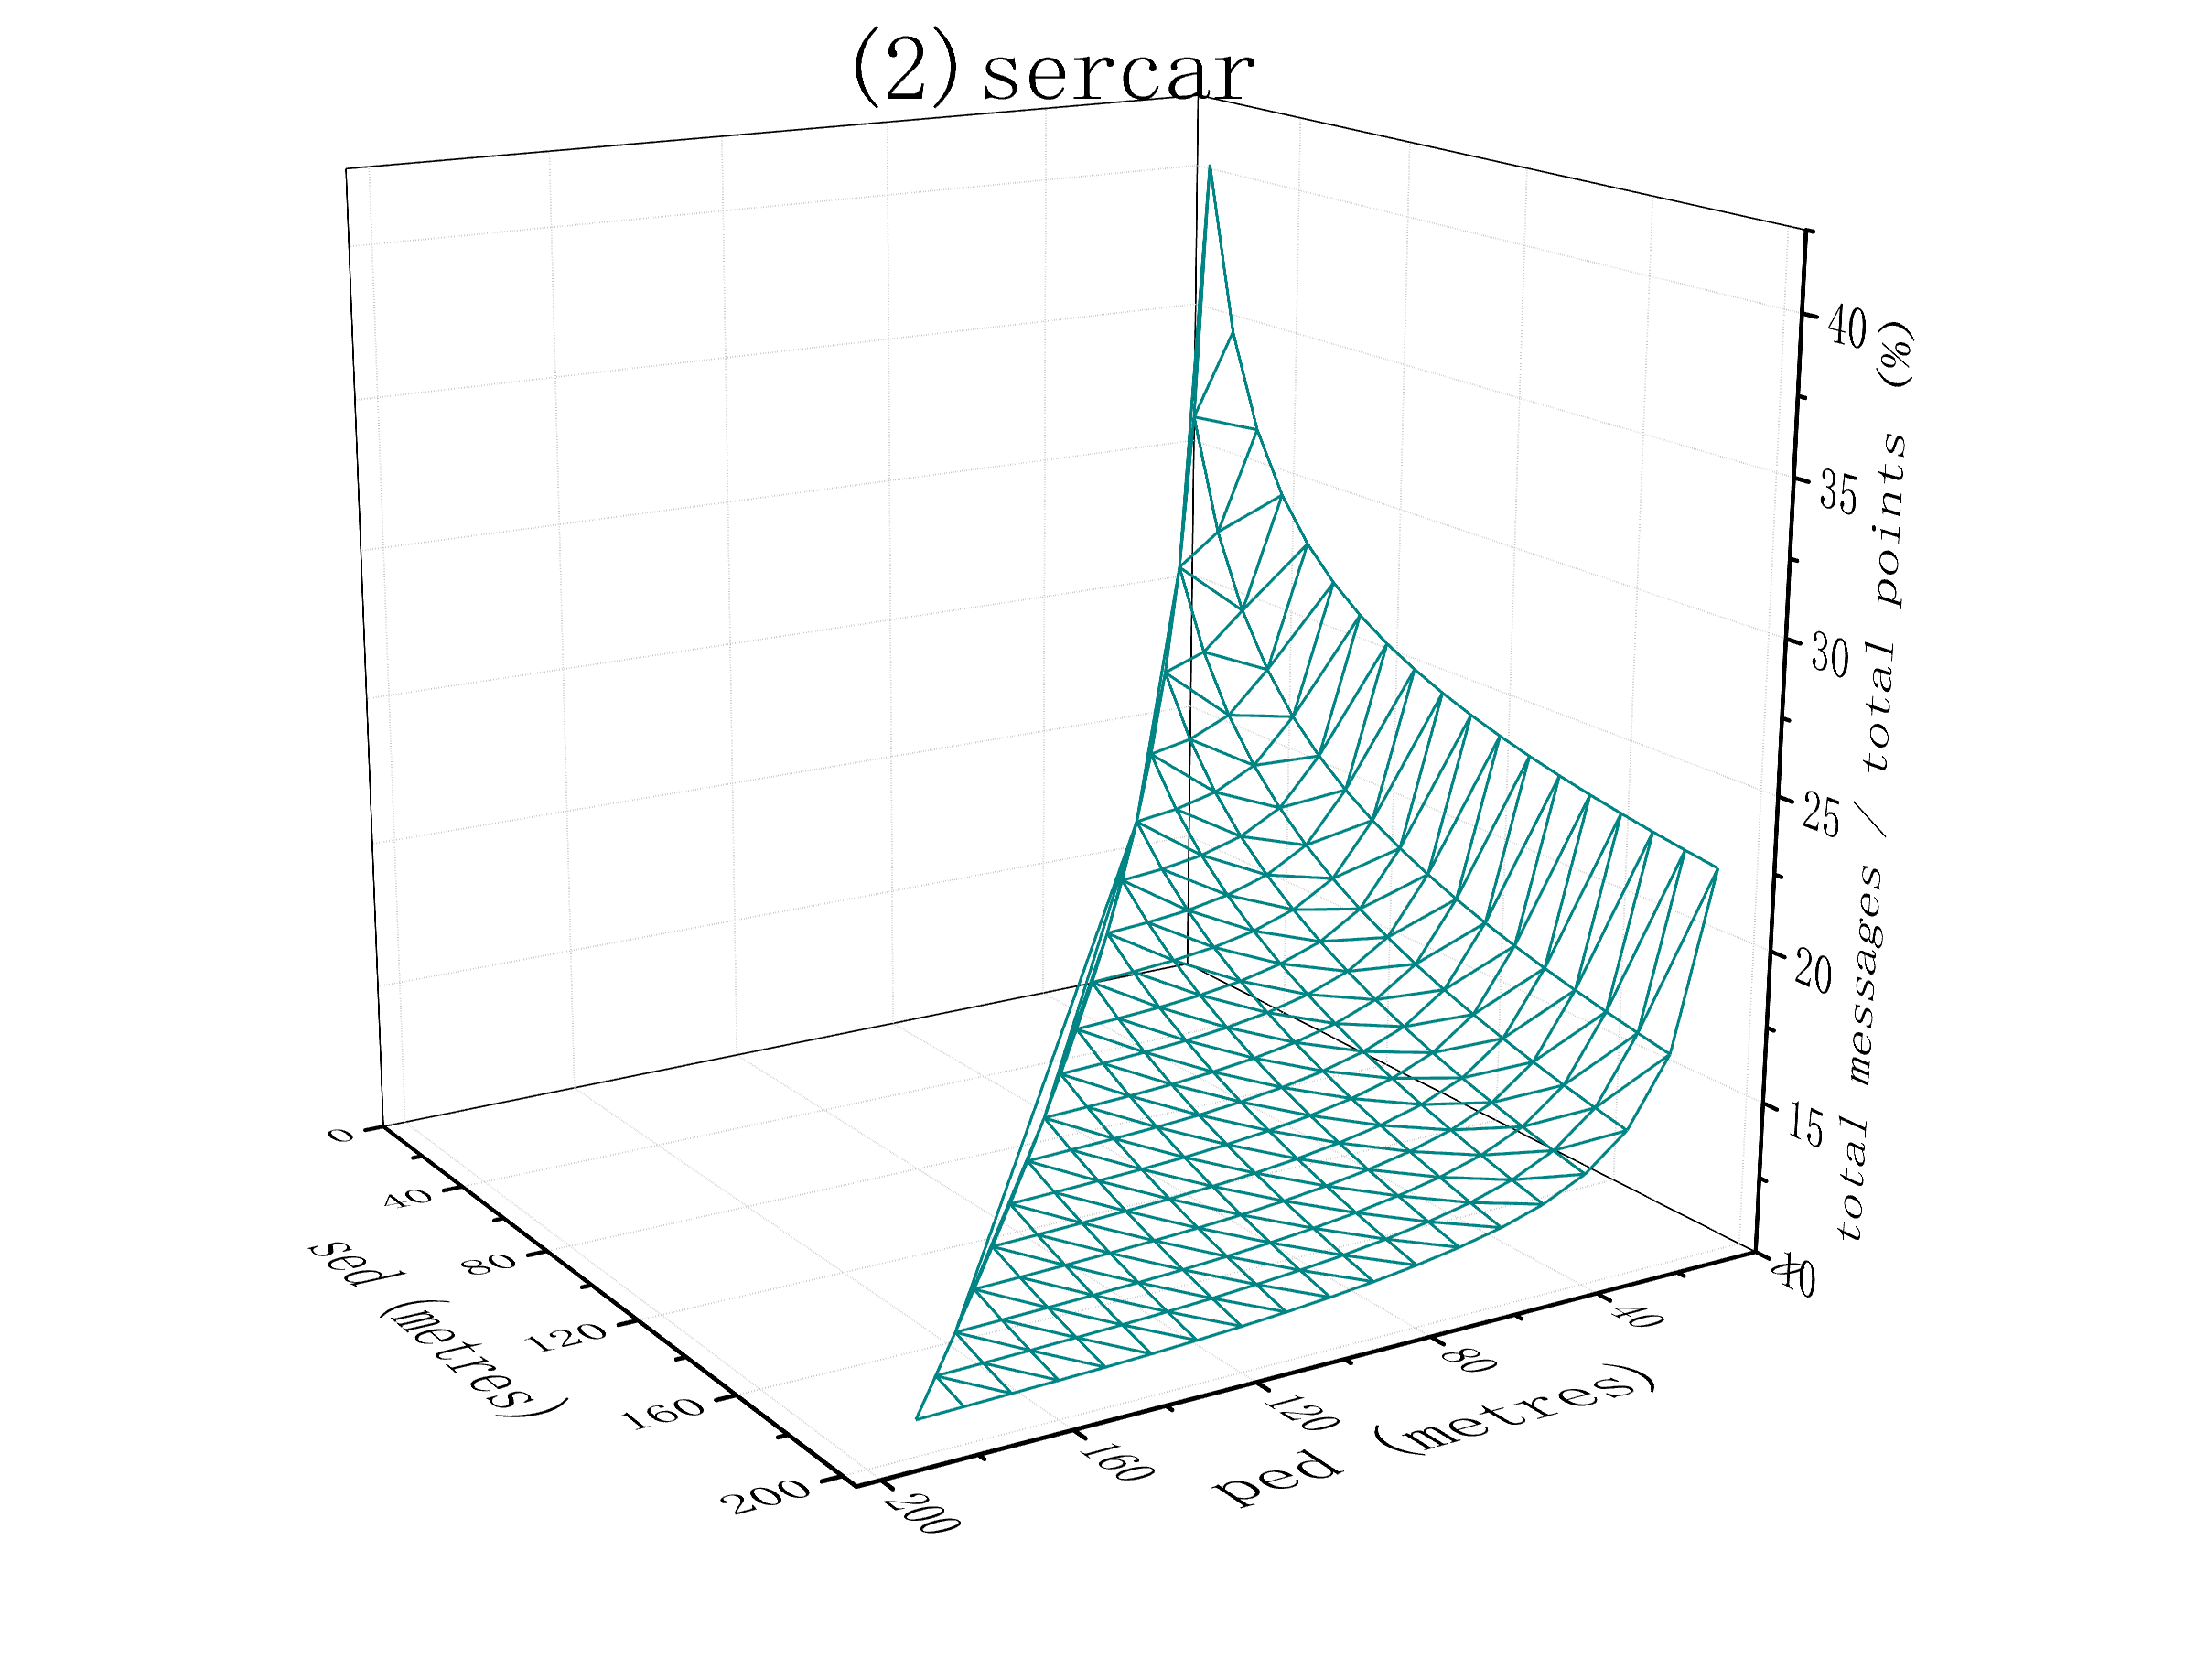
\includegraphics[scale = 0.565]{figures/Fig-BITT-sercar-total-messages.png}\hspace{1ex}
	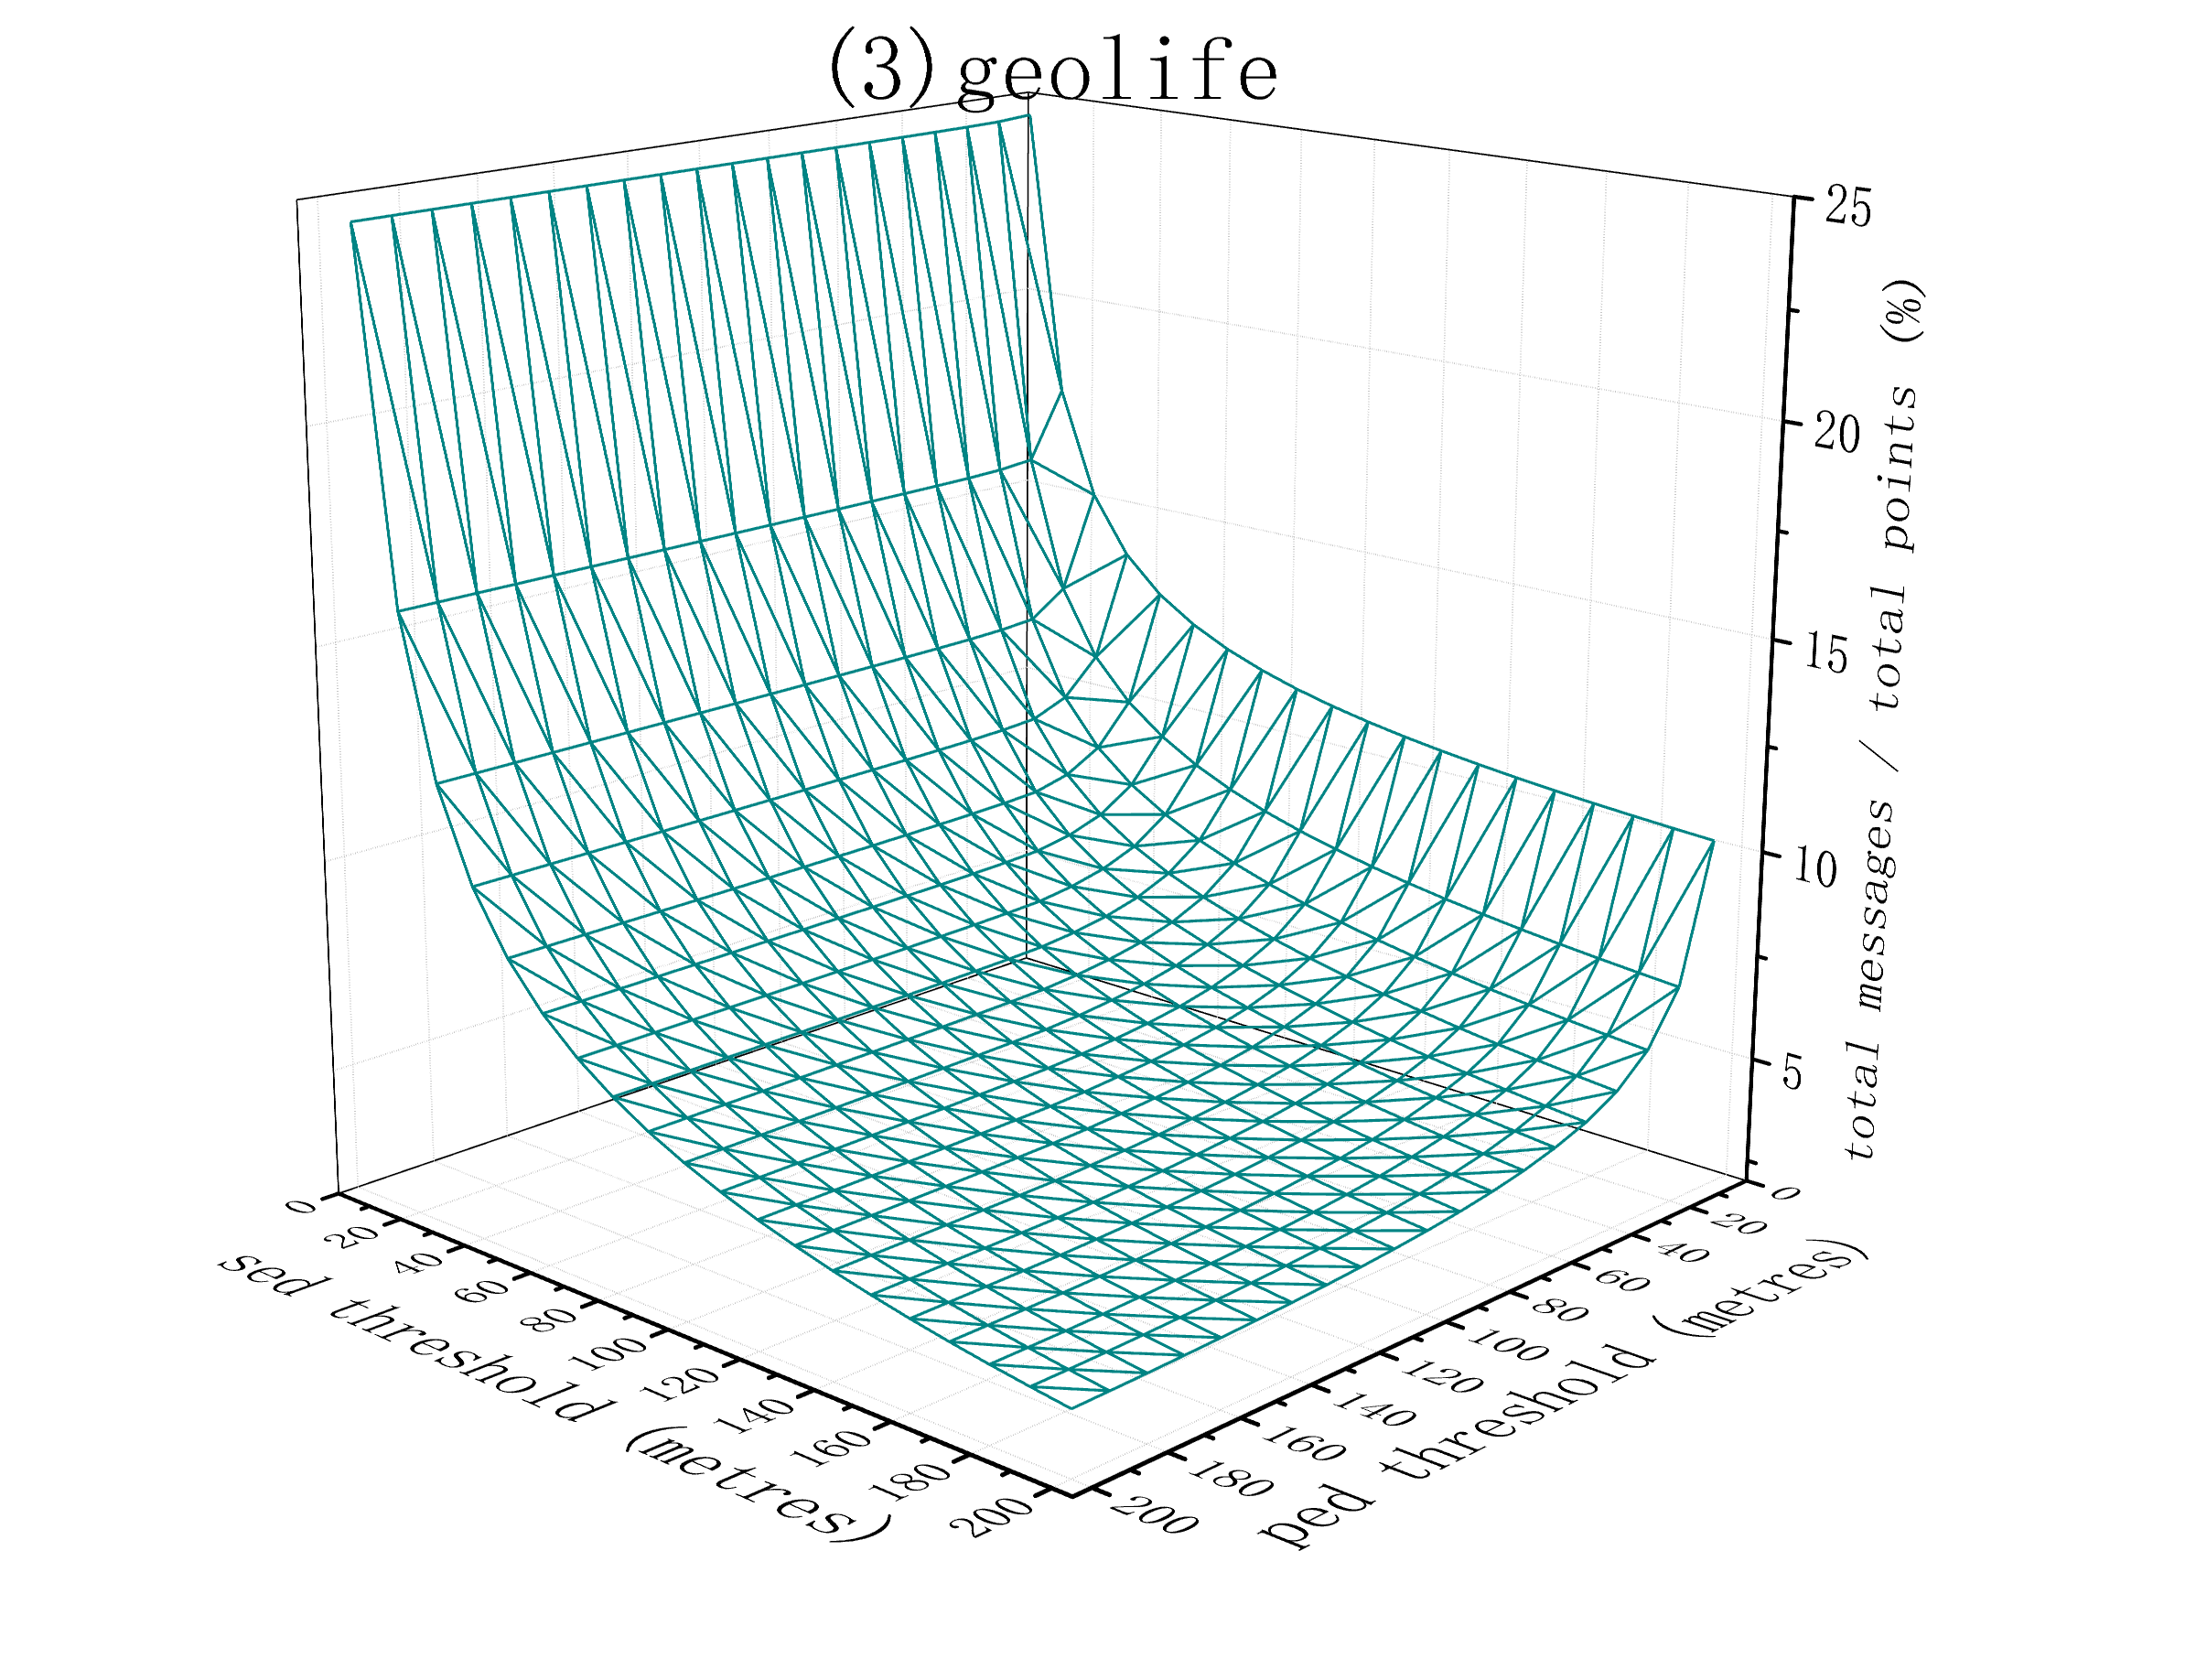
\includegraphics[scale = 0.565]{figures/Fig-BITT-geolife-total-messages.png}\hspace{1ex}
	\vspace{-2ex}
	\caption{\small Evaluation of the total messages of \bitt: varying error bounds $\epsilon_{sed}$ and $\epsilon_{ped}$.}
	\label{fig:bitt-total-message}
	\vspace{-1ex}
\end{figure*}




\begin{figure*}[tb!]
	\centering
	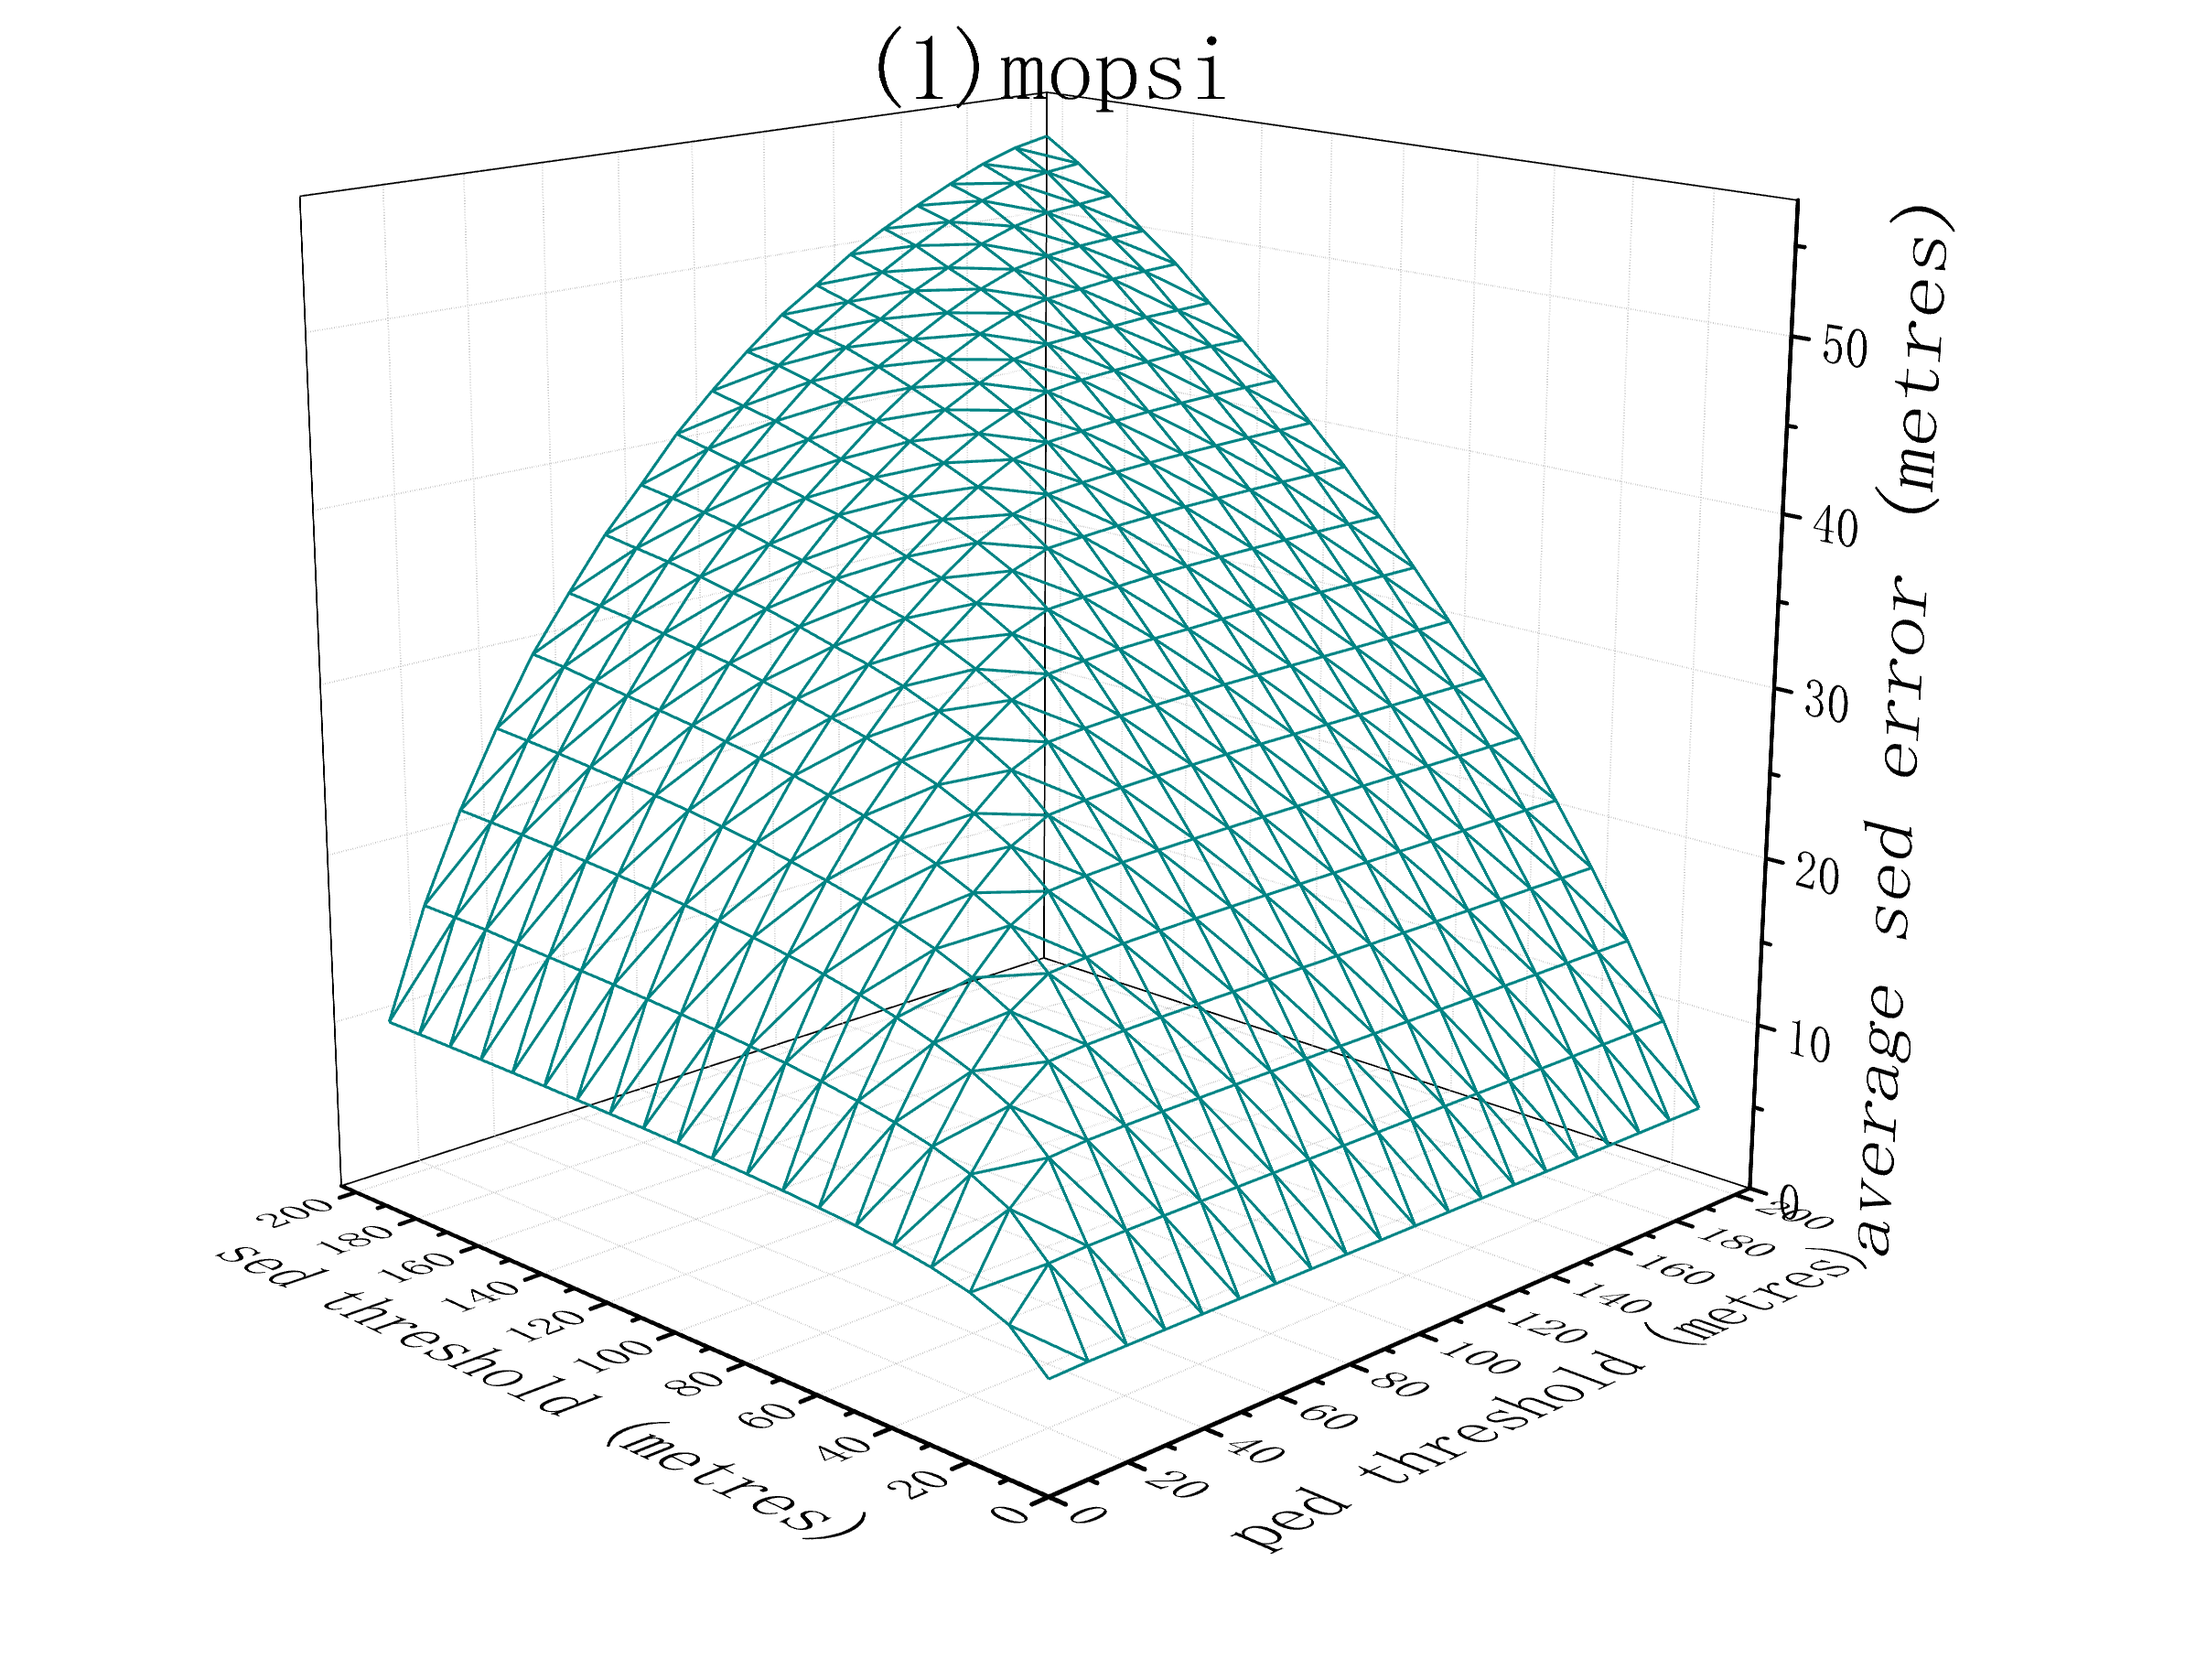
\includegraphics[scale = 0.56]{figures/Fig-BITT-mopsi-sed-error.png}\hspace{1ex}
	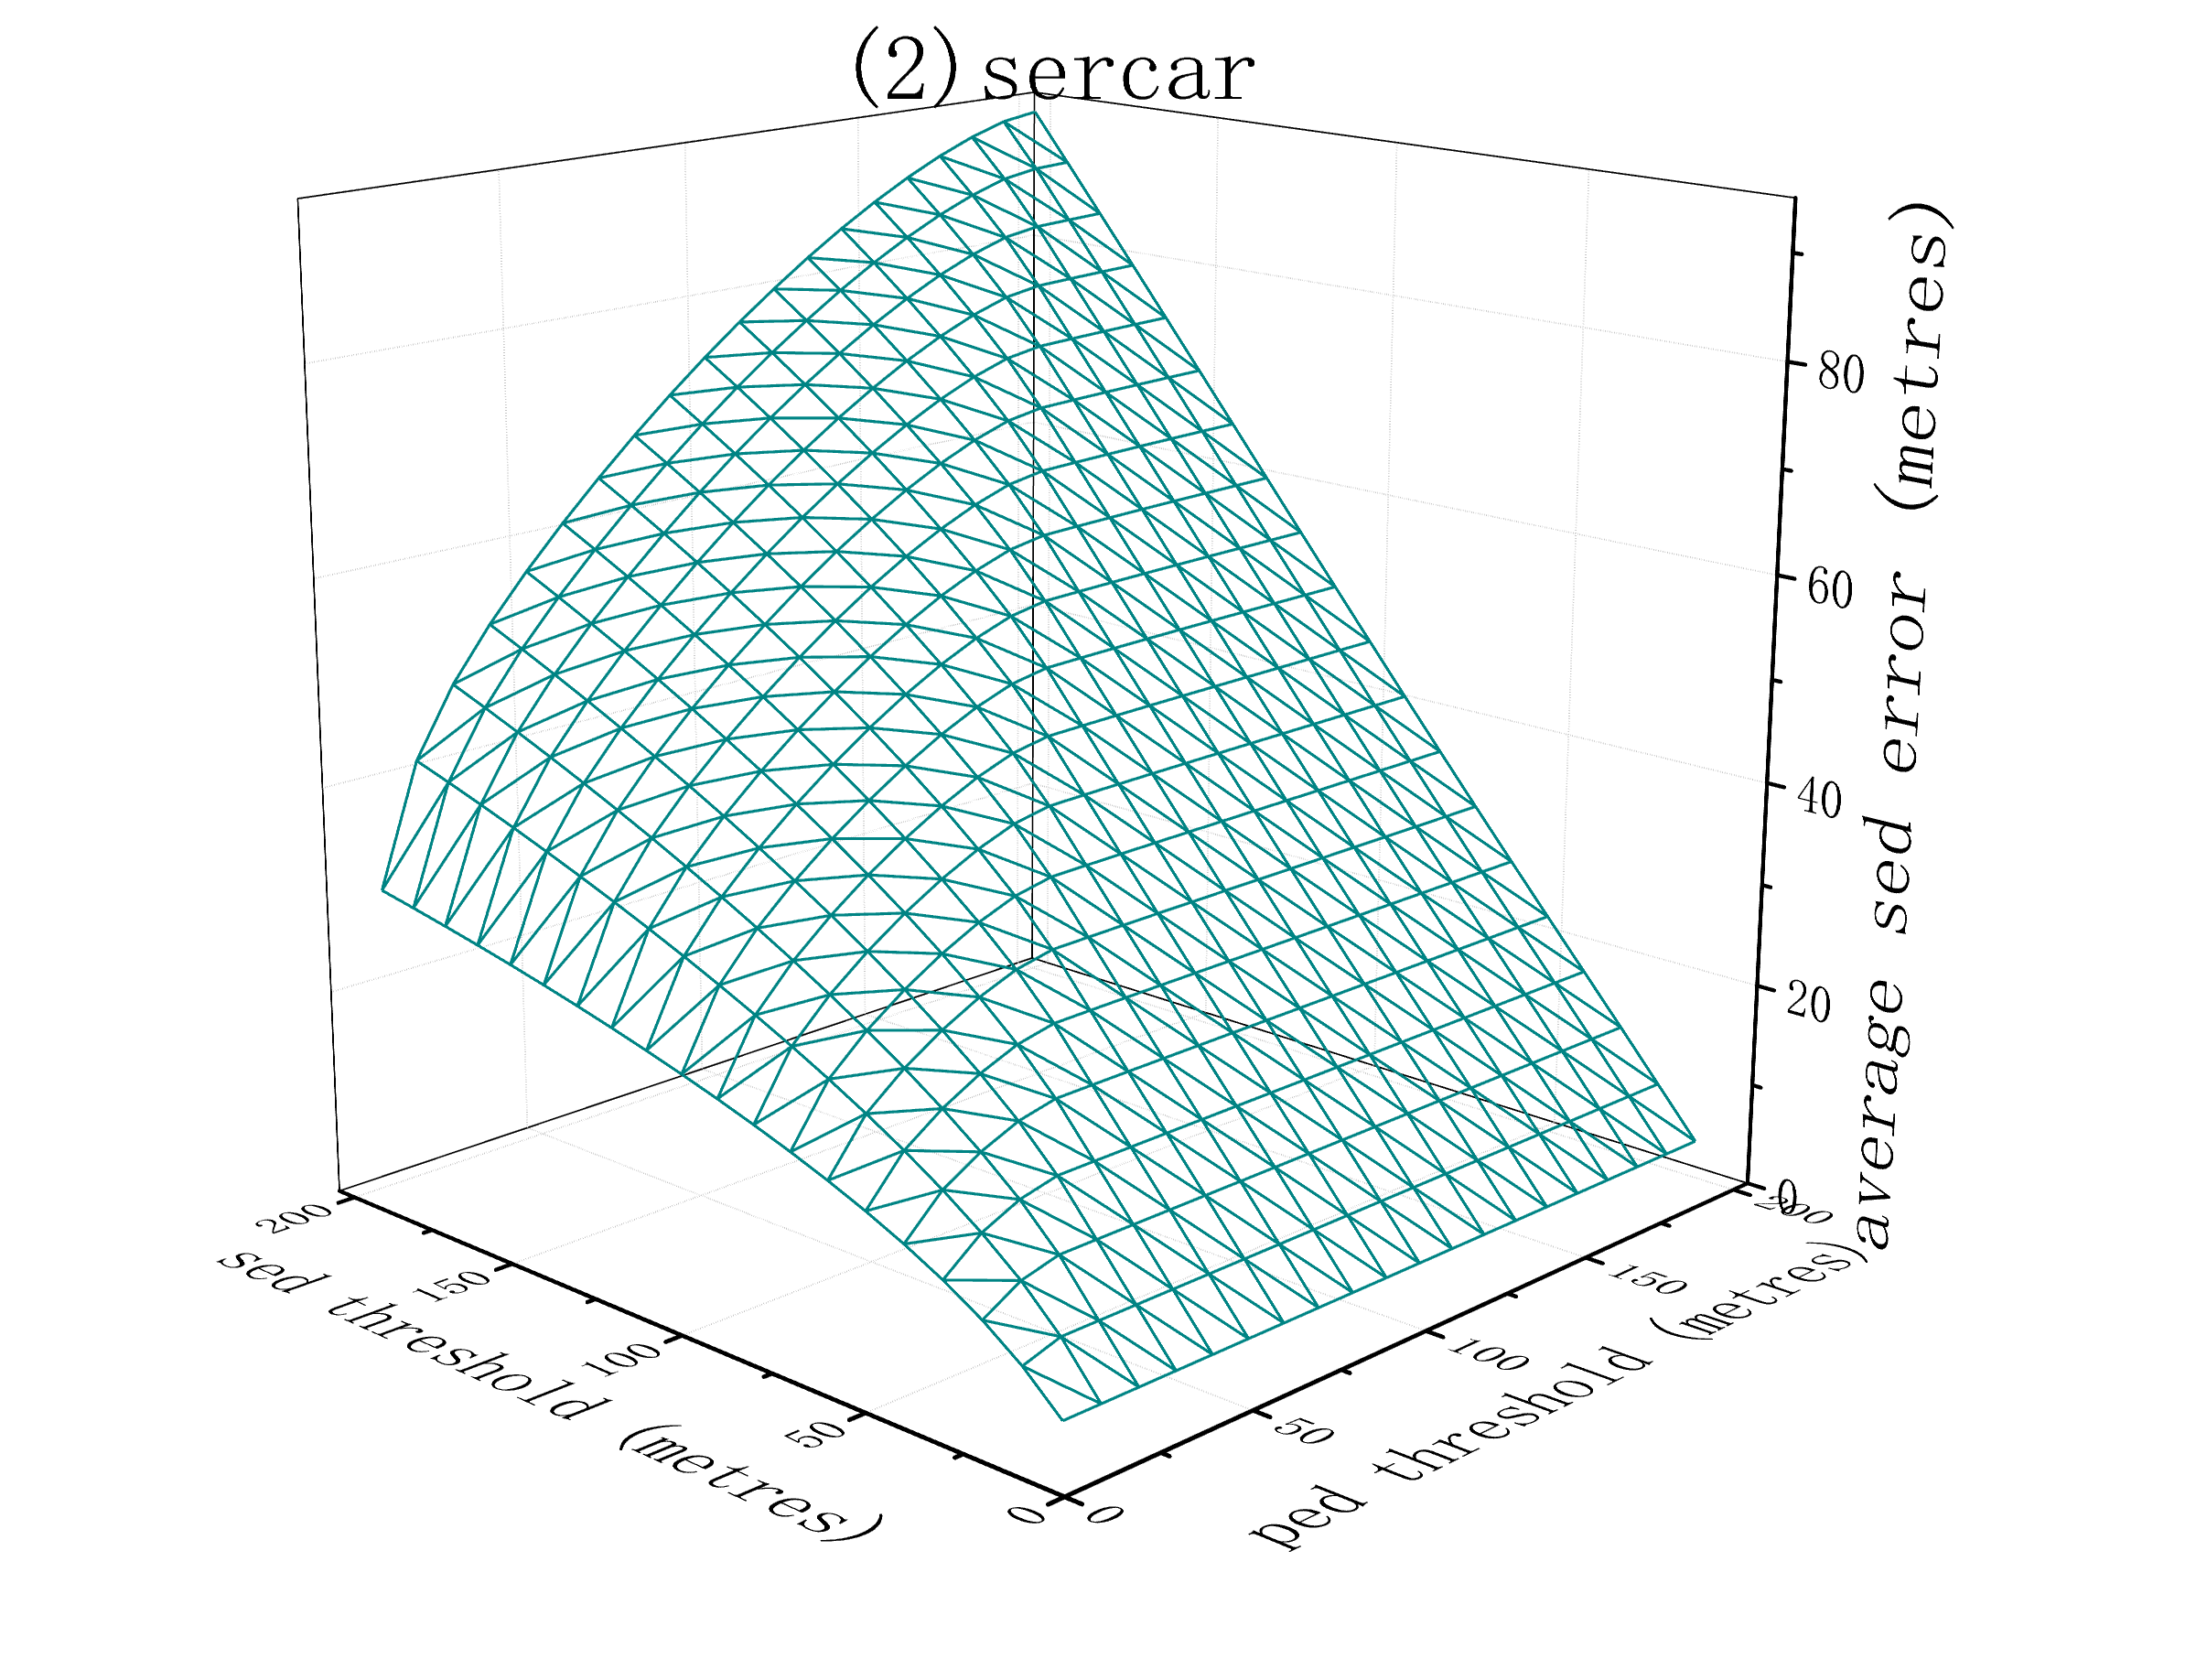
\includegraphics[scale = 0.56]{figures/Fig-BITT-sercar-sed-error.png}\hspace{1ex}
	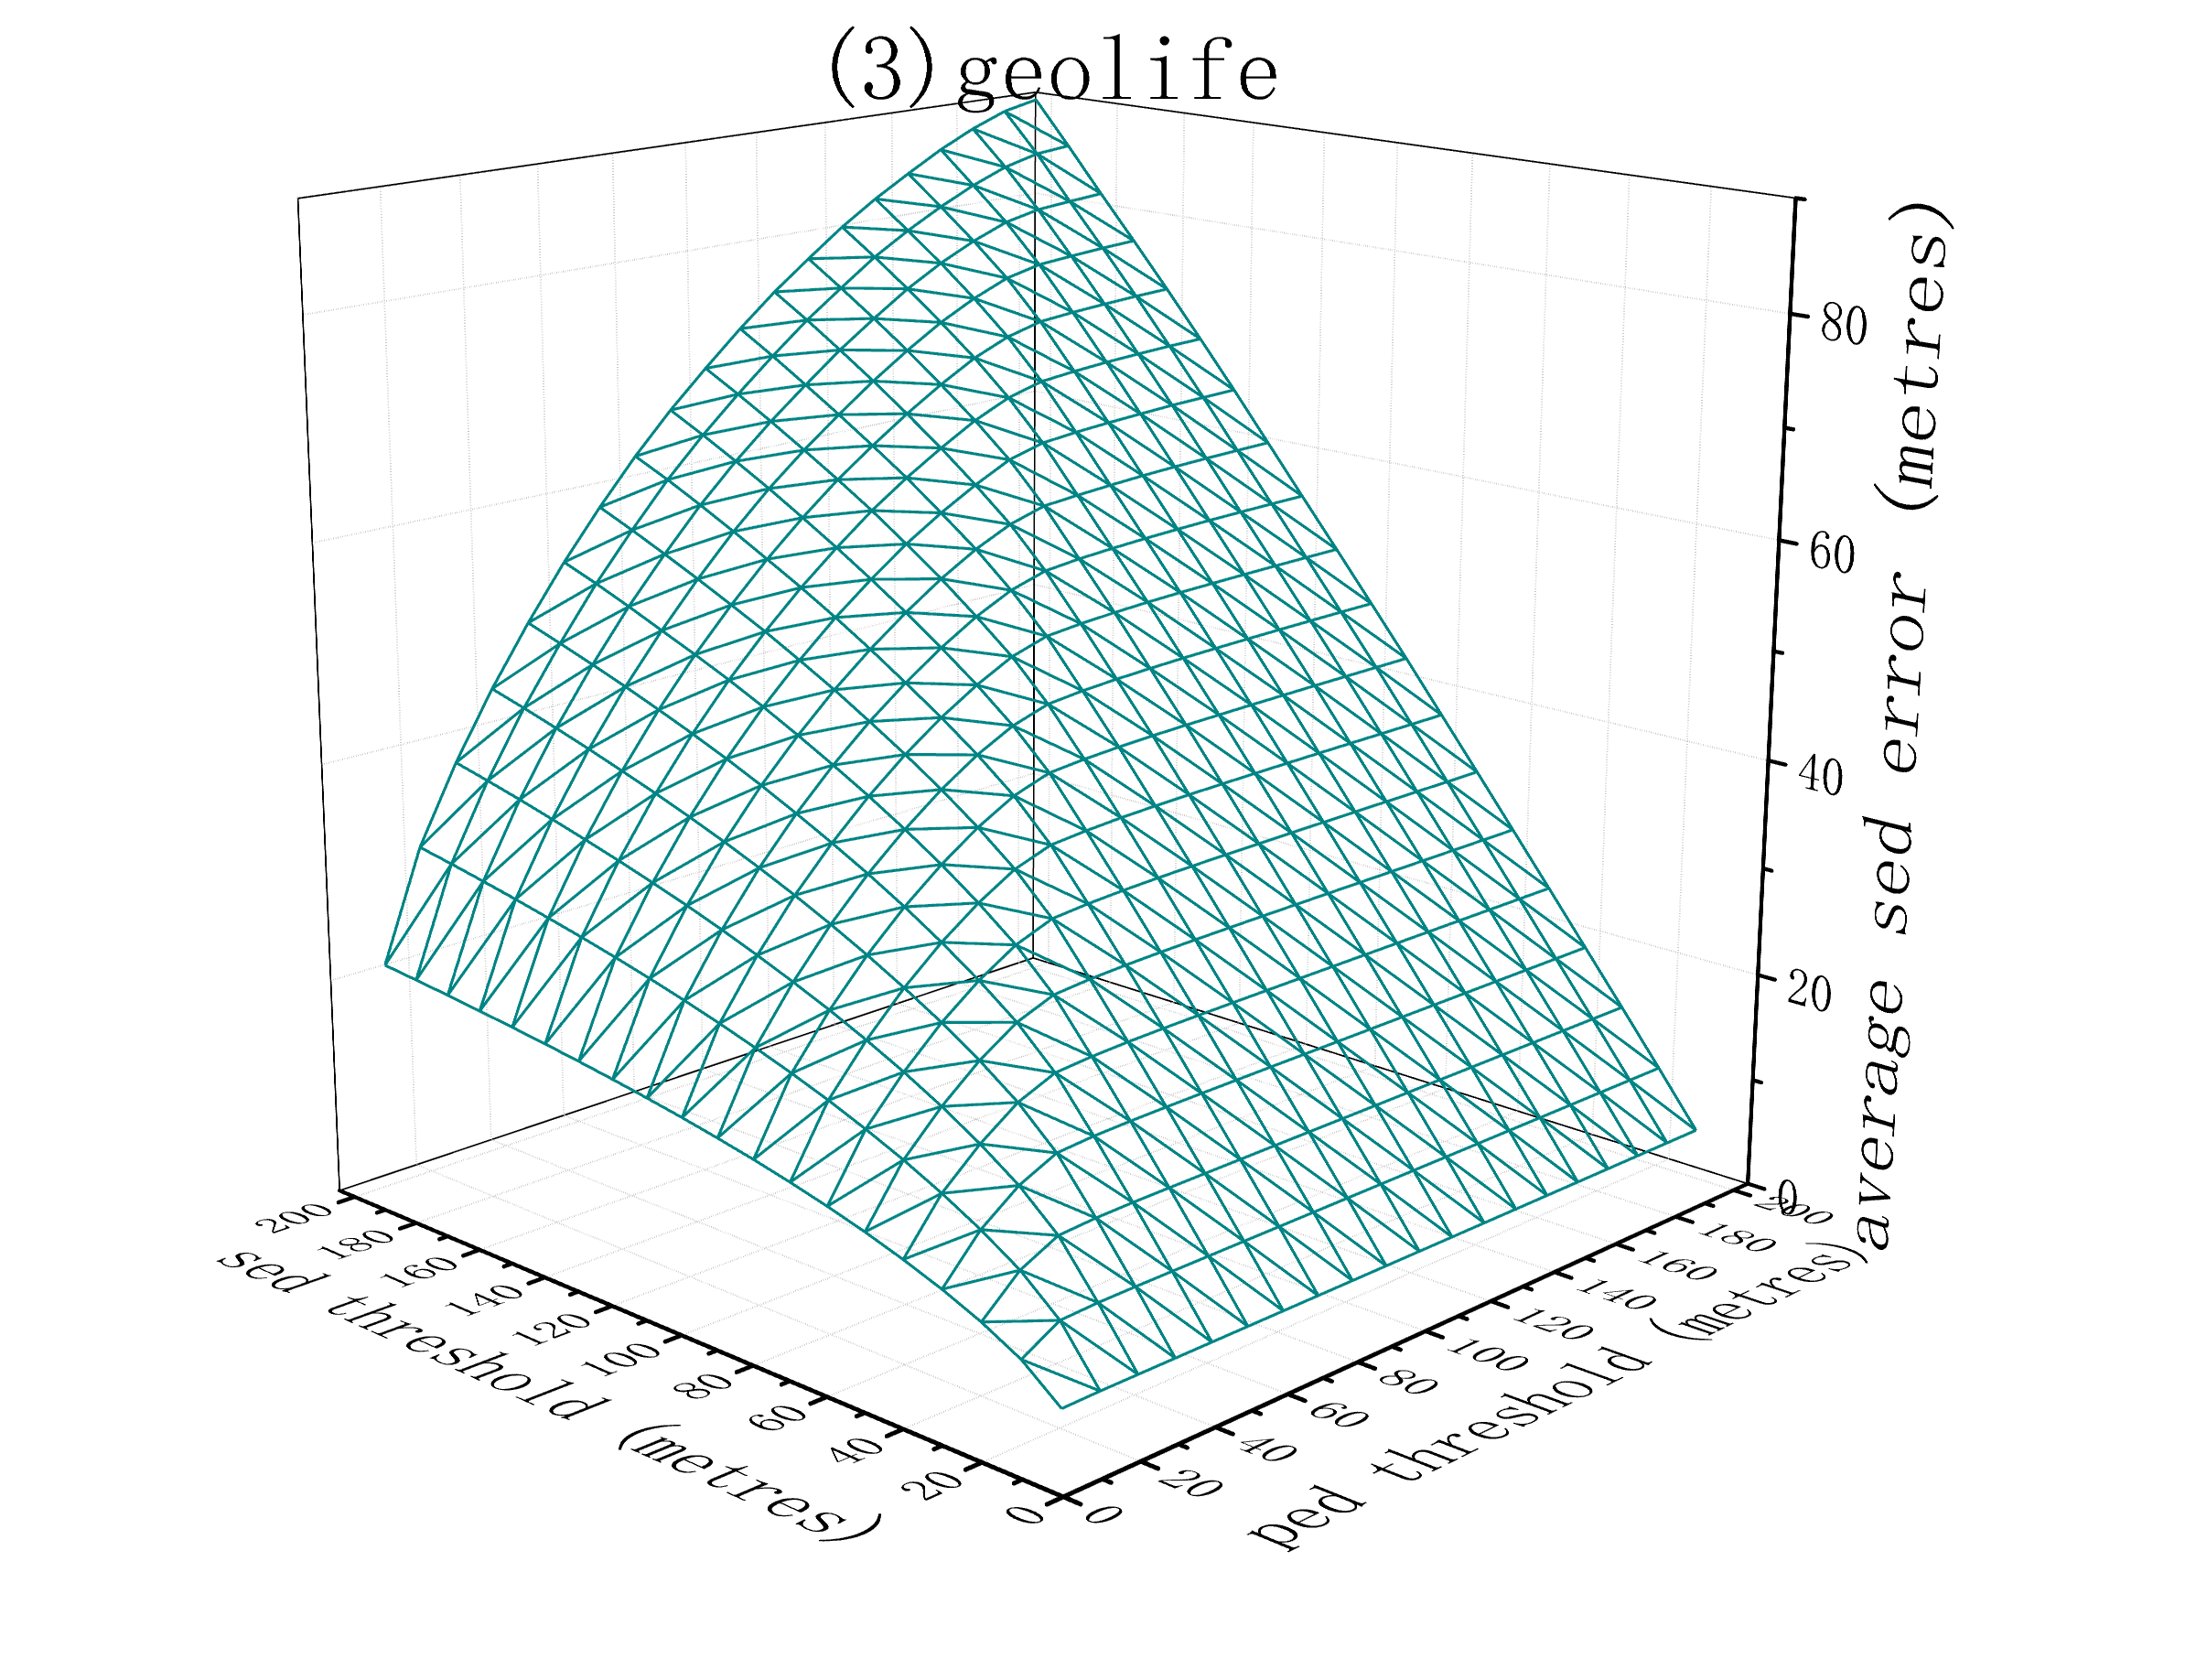
\includegraphics[scale = 0.56]{figures/Fig-BITT-geolife-sed-error.png}\hspace{1ex}
	\vspace{-2ex}
	\caption{\small Evaluation of the \sed errors of \bitt: varying error bounds $\epsilon_{sed}$ and $\epsilon_{ped}$.}
	\label{fig:bitt-sed-error}
	\vspace{-1ex}
\end{figure*}



\begin{figure*}[tb!]
	\centering
	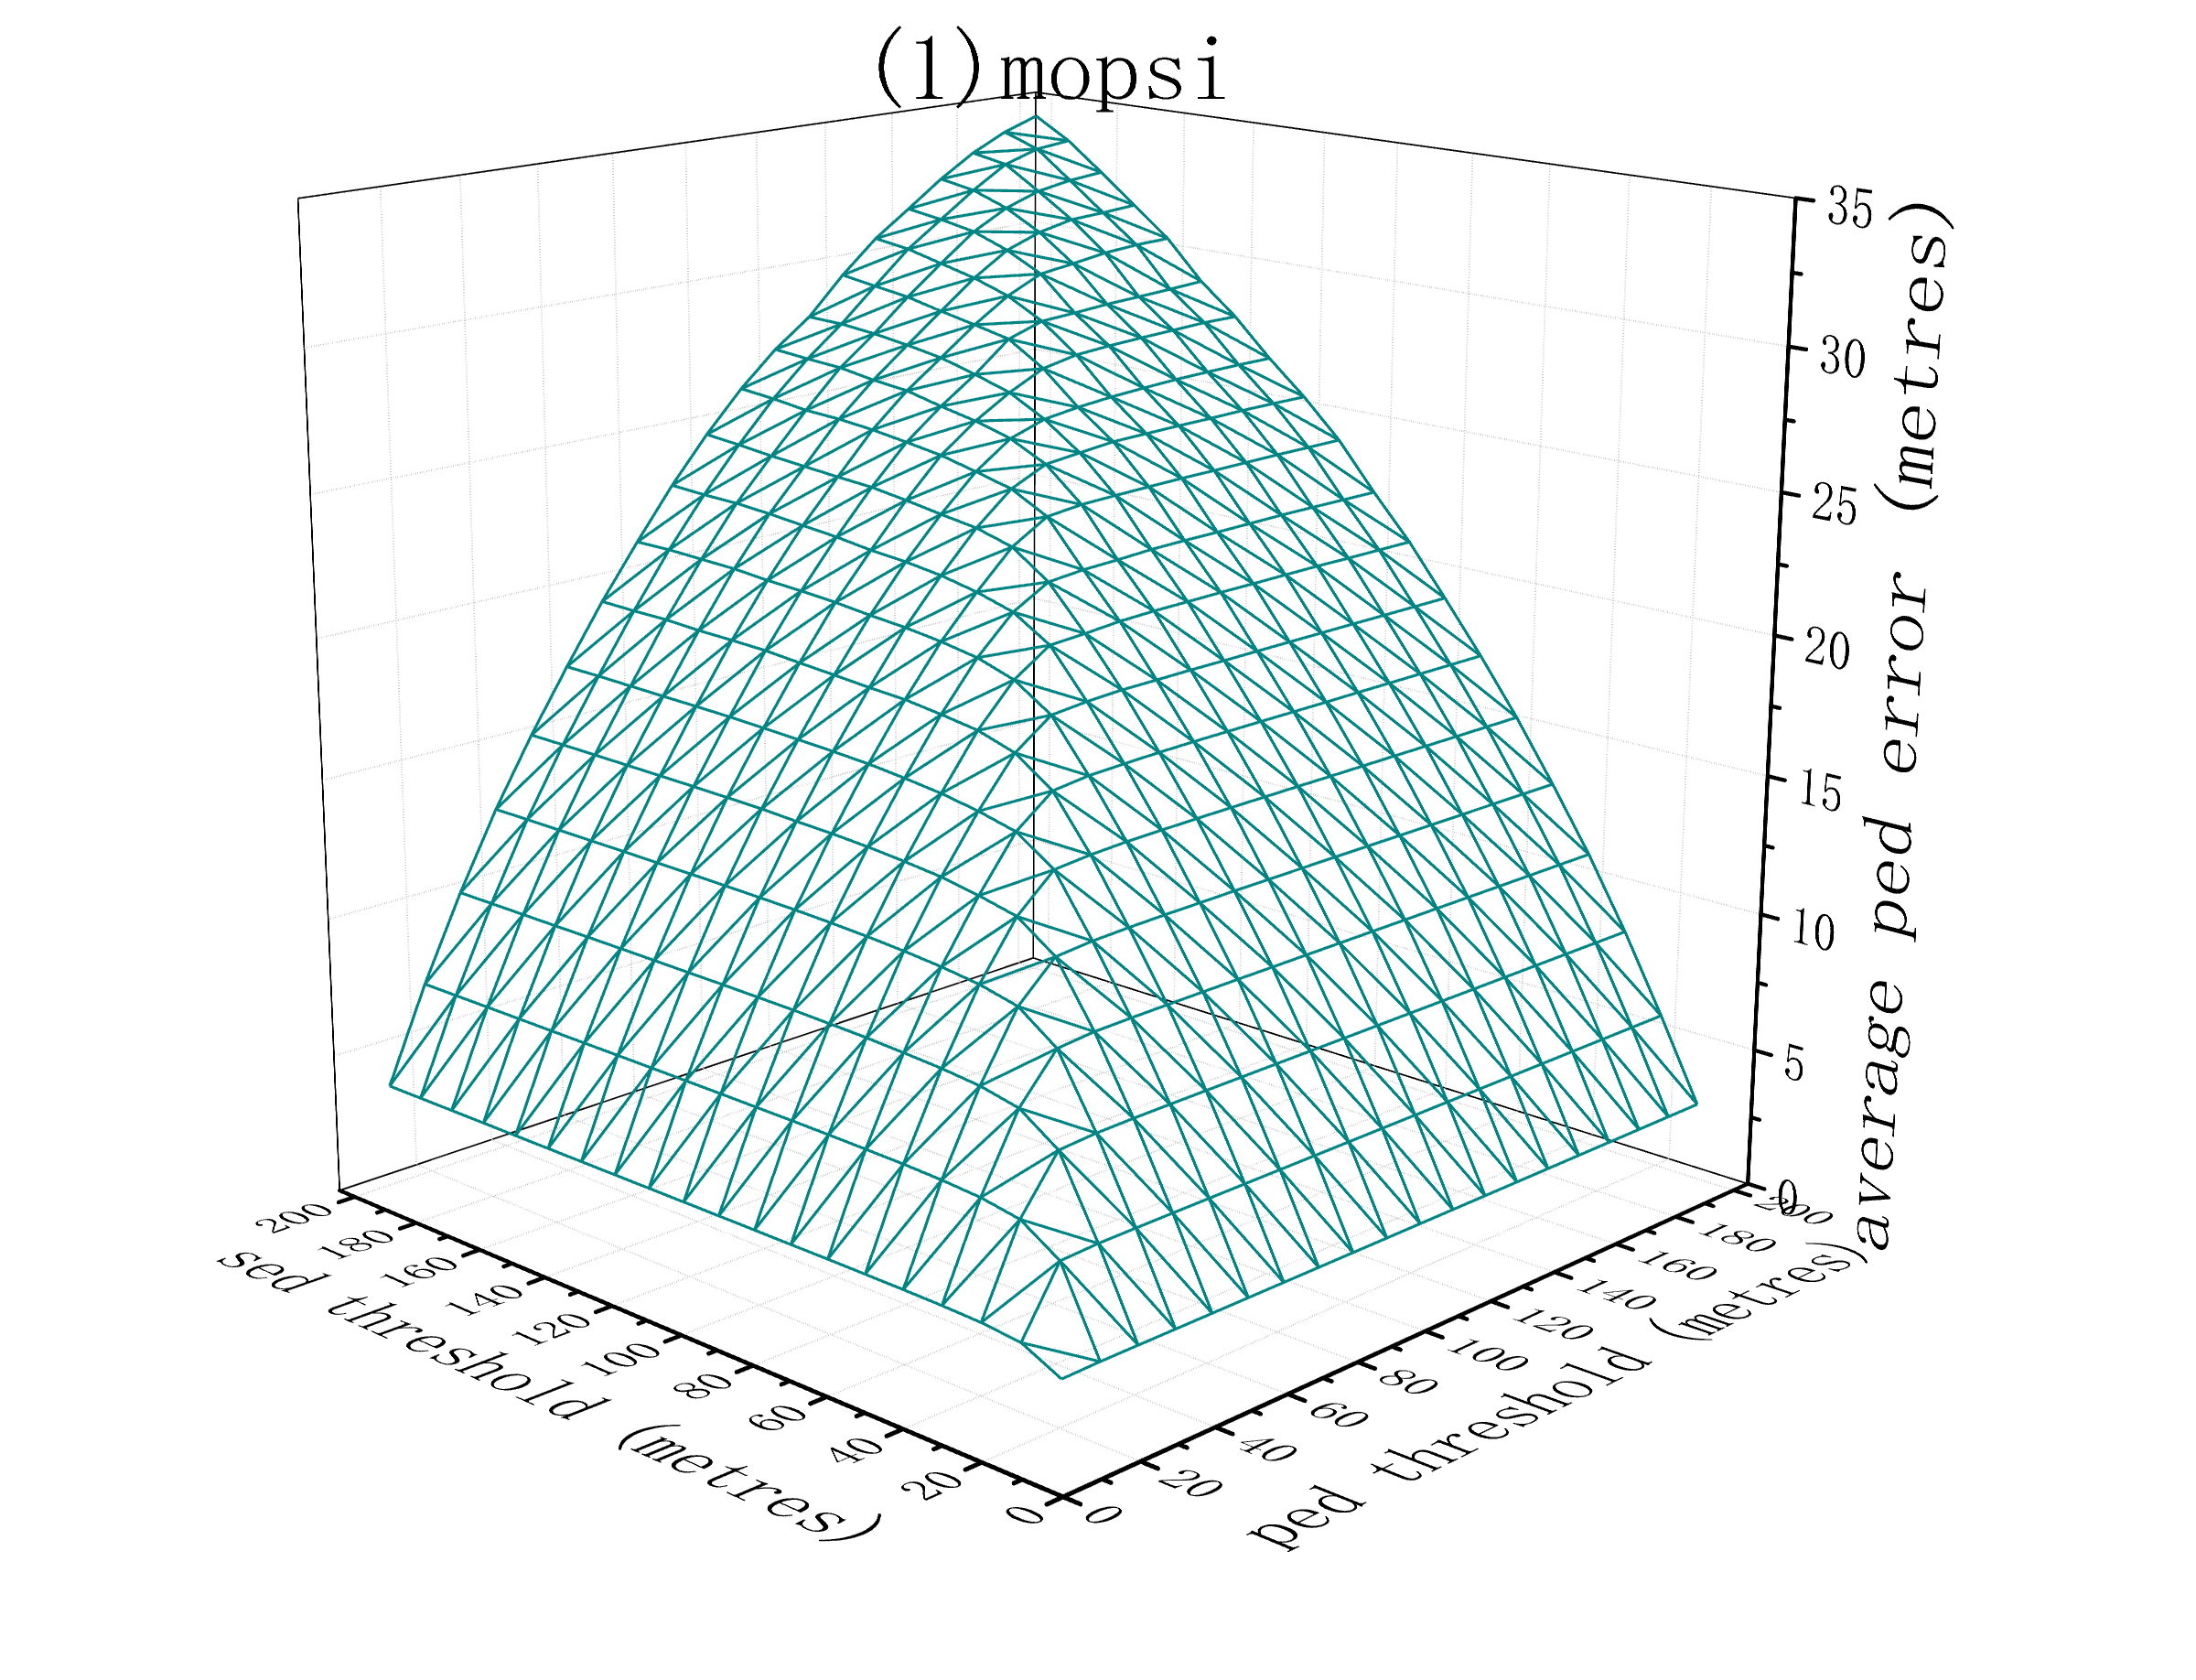
\includegraphics[scale = 0.56]{figures/Fig-BITT-mopsi-ped-error.png}\hspace{1ex}
	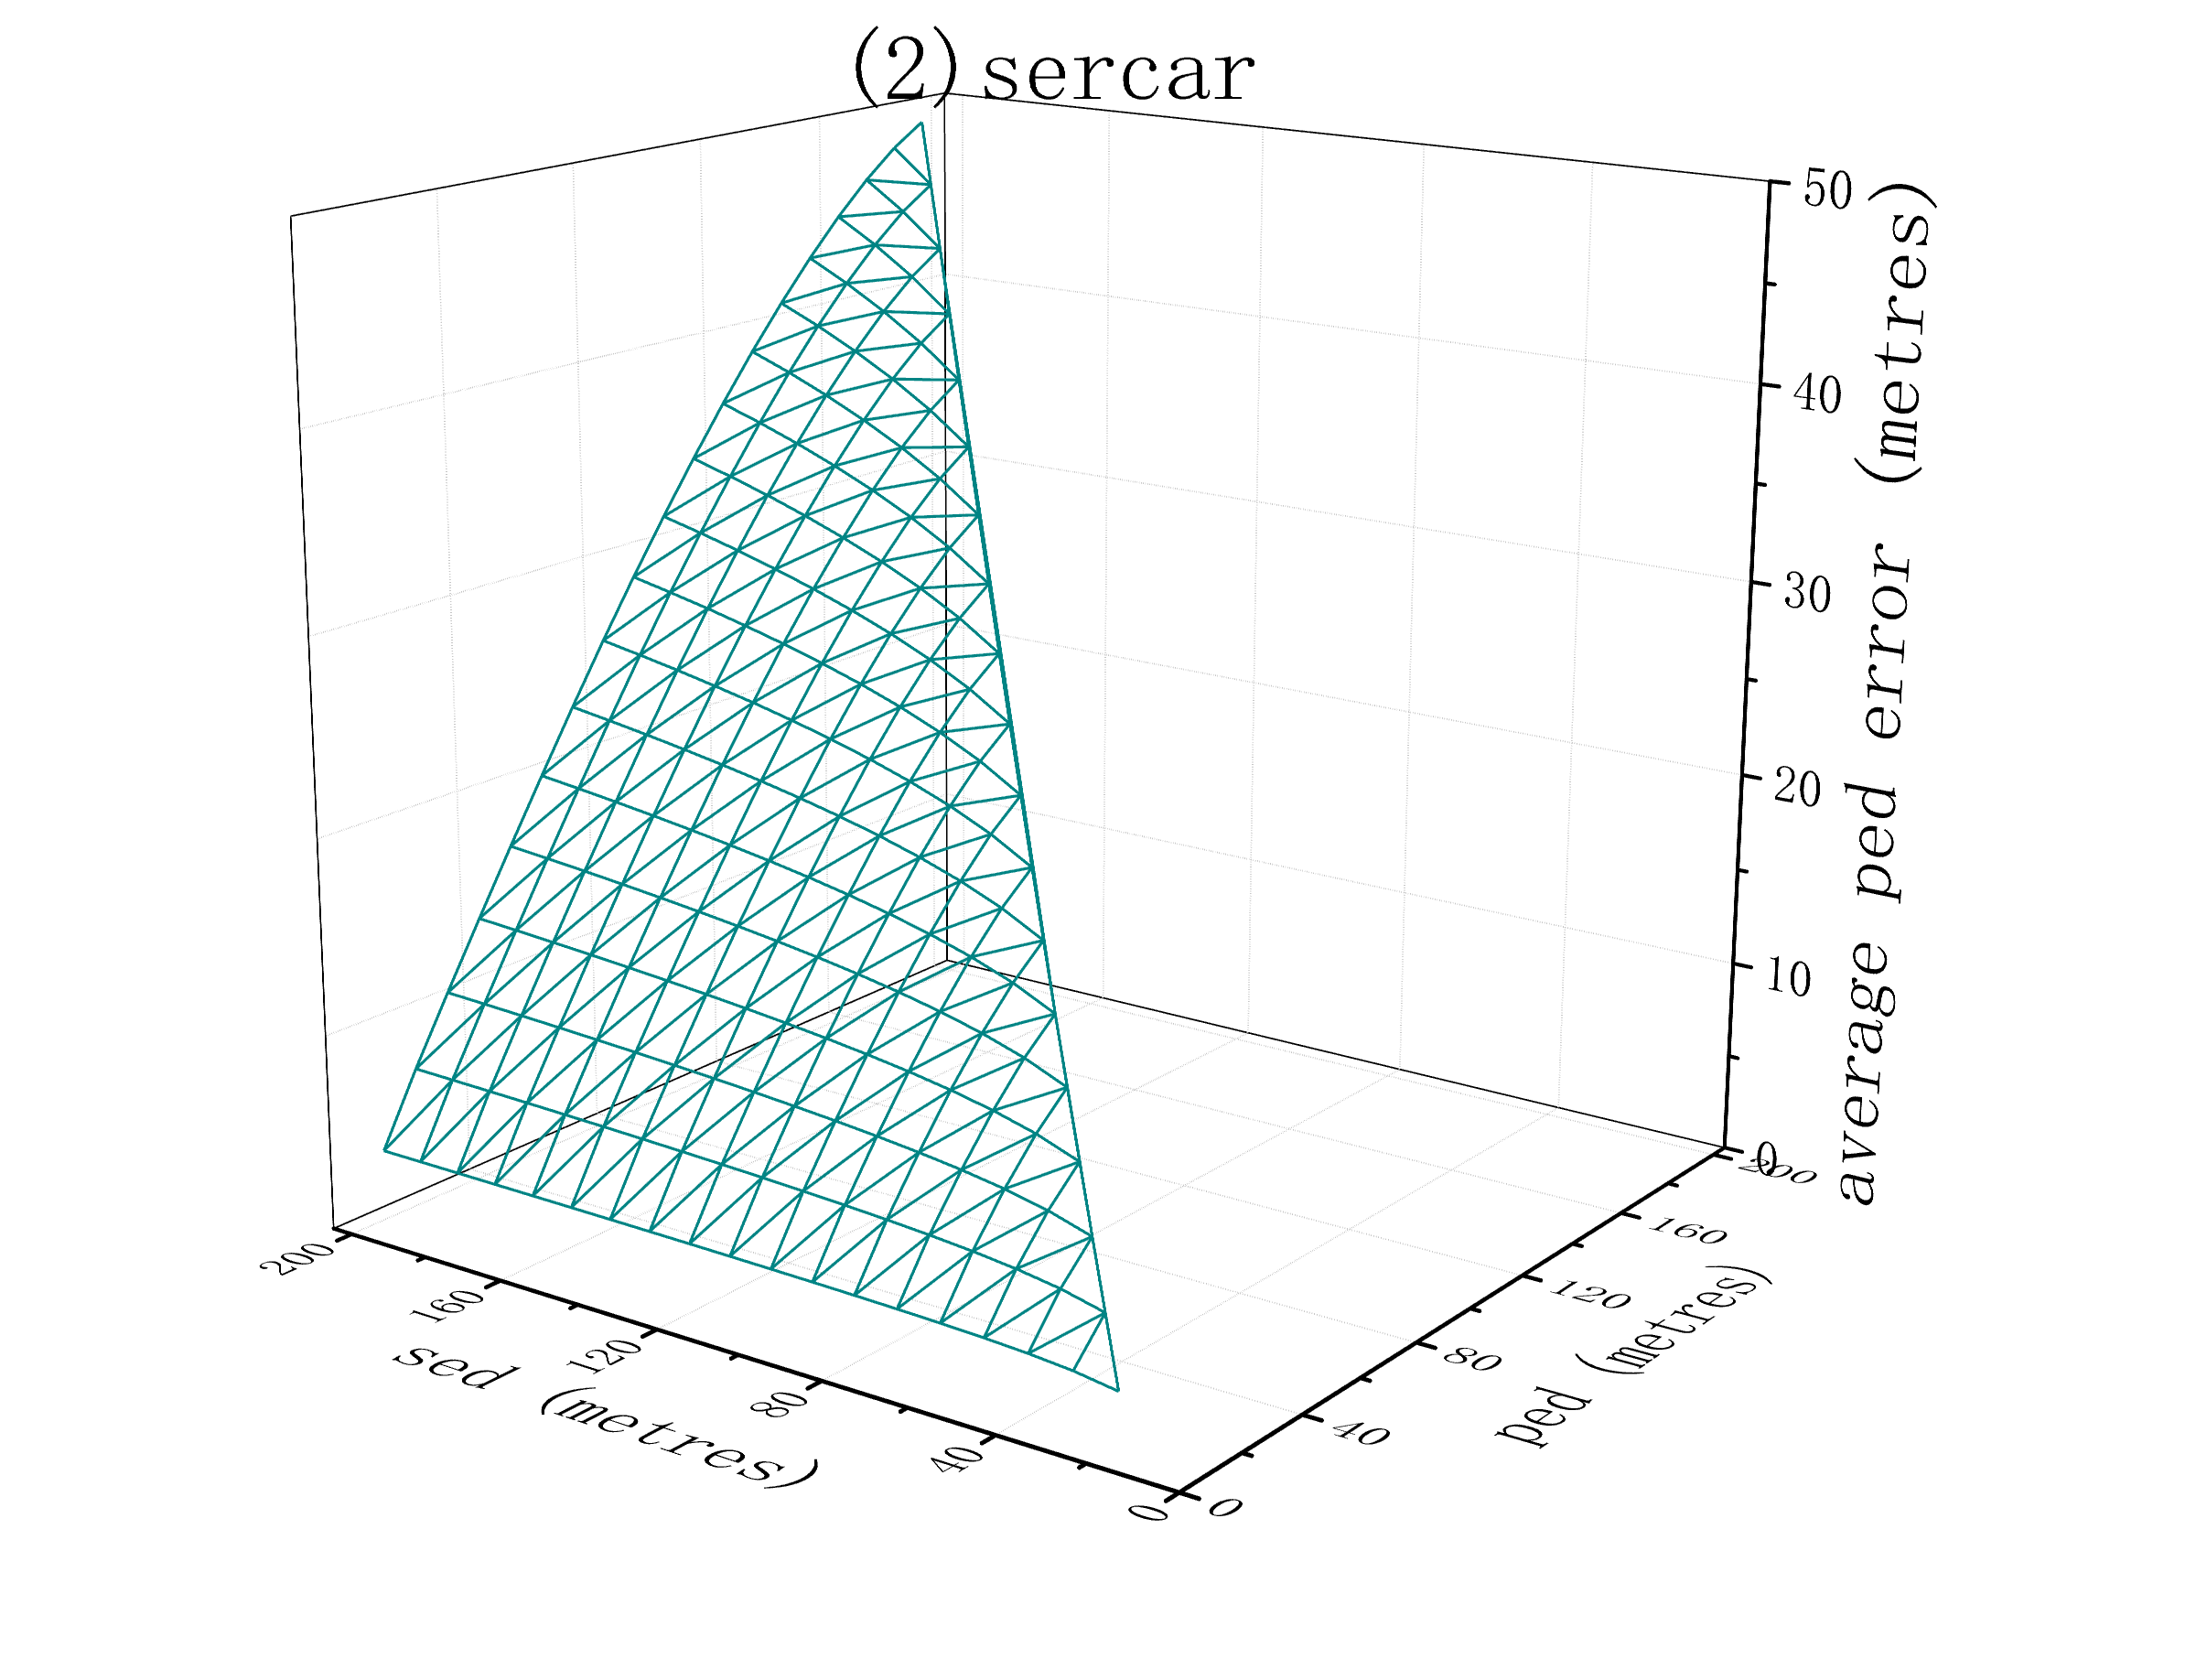
\includegraphics[scale = 0.56]{figures/Fig-BITT-sercar-ped-error.png}\hspace{1ex}
	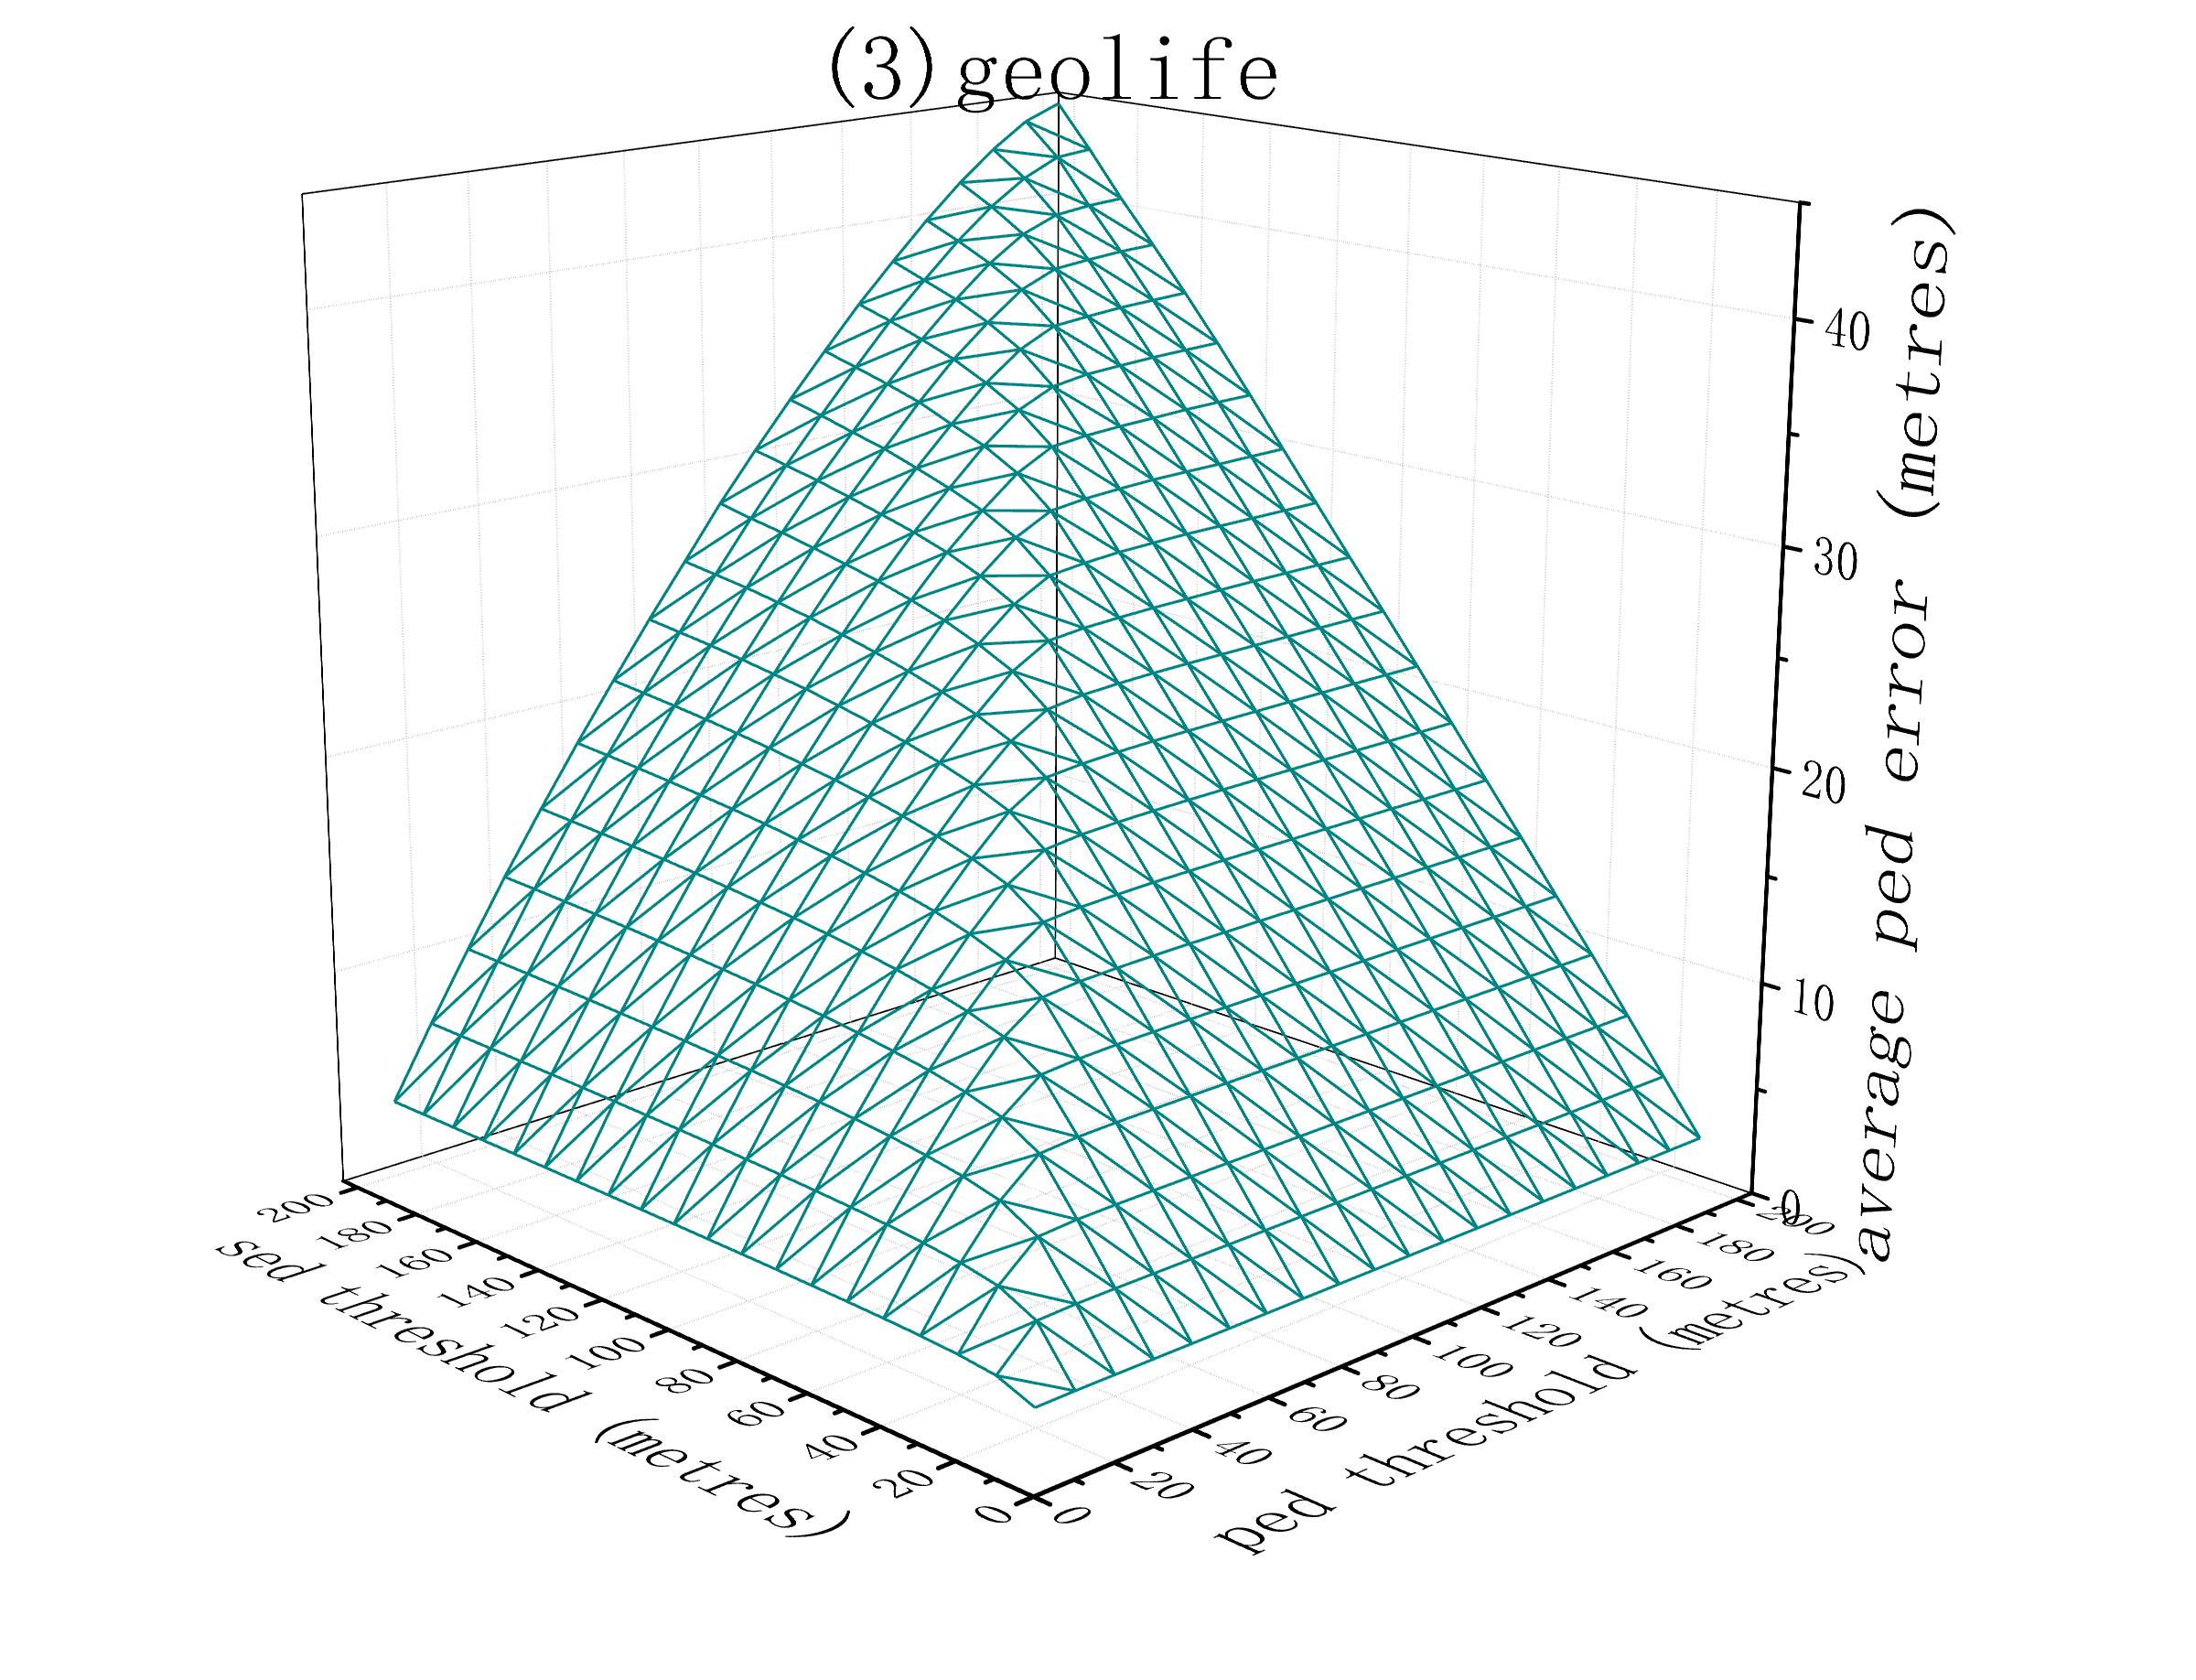
\includegraphics[scale = 0.56]{figures/Fig-BITT-geolife-ped-error.png}\hspace{1ex}
	\vspace{-2ex}
	\caption{\small Evaluation of the \ped errors of \bitt: varying error bounds $\epsilon_{sed}$ and $\epsilon_{ped}$.}
	\label{fig:bitt-ped-error}
	\vspace{-1ex}
\end{figure*}

\subsection{Experimental setting}

\stitle{Real-life Trajectory Datasets}. We use three reallife datasets ServiceCar, GeoLife and Mopsi shown in Table \ref{tab:datasets} to test our solutions.

\vspace{0.5ex}
\ni \emph{(1) Service car trajectory data} (\sercar) is the GPS trajectories collected by a Chinese car rental company during Apr. 2015 to Nov. 2015. The sampling rate was one point per $3$--$5$ seconds, and
each trajectory has around $114.1K$ points.

\vspace{0.5ex}
\ni \emph{(2) GeoLife trajectory data} (\geolife) is the GPS trajectories collected in GeoLife project by 182 users in a period from Apr. 2007 to Oct. 2011. These trajectories have a variety of sampling rates, among which 91\% are logged in each 1-5 seconds per point. %or each 5-10 meters

\vspace{0.5ex}
\ni \emph{(3) Mopsi trajectory data} (\mopsi) is the GPS trajectories collected in Mopsi project by 51 users in a period from 2008 to 2014. Most routes are in Joensuu region, Finland.
The sampling rate was one point per $2$ seconds, and each trajectory has around $153.9K$ points.

\stitle{Algorithms and implementation}.
We implement five tracking algorithms, \ie our \citt, \sitt and \bitt, \ldrh \cite{Trajcevski:LDRH} (the first and the most efficient trajectory tracking algorithm) and \grts~\cite{Lange:GRTS,Lange:Tracking} (the most effective tracking algorithm).
All algorithms were implemented with Java.
All tests were run on an {x64-based  PC with 8 Intel(R) Core(TM) i5-6500 CPU @ 3.20GHz and 8GB of memory.
	%, and each test was repeated over 3 times and the average is reported here.
	
\stitle{Metrics.}
Following the main stream \cite{Trajcevski:LDRH, Lange:GRTS, Lange:Tracking, Lin:Cised, Zhang:Evaluation}, we use \emph{compression ratio}, \emph{message ratio}, \emph{error} and \emph{running time} to evaluate algorithms.

 \ni \emph{(1) Compression ratio}. {It is defined as follows: Given a set of trajectories $\{\dddot{\mathcal{T}_1}, \ldots, \dddot{\mathcal{T}_M}\}$ and their piece-wise line representations $\{\overline{\mathcal{T}_1}, \ldots, \overline{\mathcal{T}_M}\}$, the compression ratio of an algorithm is $(\sum_{j=1}^{M} |\overline{\mathcal{T}}_j |)/(\sum_{j=1}^{M} |\dddot{\mathcal{T}}_j |)$.
	By the definition, \emph{algorithms with lower compression ratios are better}.}

 \ni \emph{(2) Message ratio}. It is ``the total number of messages'' divided by ``the total number of the original trajectory points''. Note there are totally three kinds of messages, \ie a) \emph{position-message} $P_s$ for \grts, b) \emph{velocity-message} $\vv{v}$ for \bitt (including \citt and \sitt) and c) \emph{position-velocity-message} ($P_s$, $\vv{v}$) for \ldrh, \grts and \bitt. 
 %For fair comparison, a \emph{position-velocity-message}
 

 \ni \emph{(3) Max and average errors}. Max (average) error is the maximal (average) value of the distances from every point of the original trajectories to its representing line segment of the simplified trajectories.
 
 \ni \emph{(4) Running time}. It is the essential execution time of an algorithm in processing a dataset.
 %It is the efficiency  of the algorithms.
 



\begin{figure*}[tb!]
	\centering
	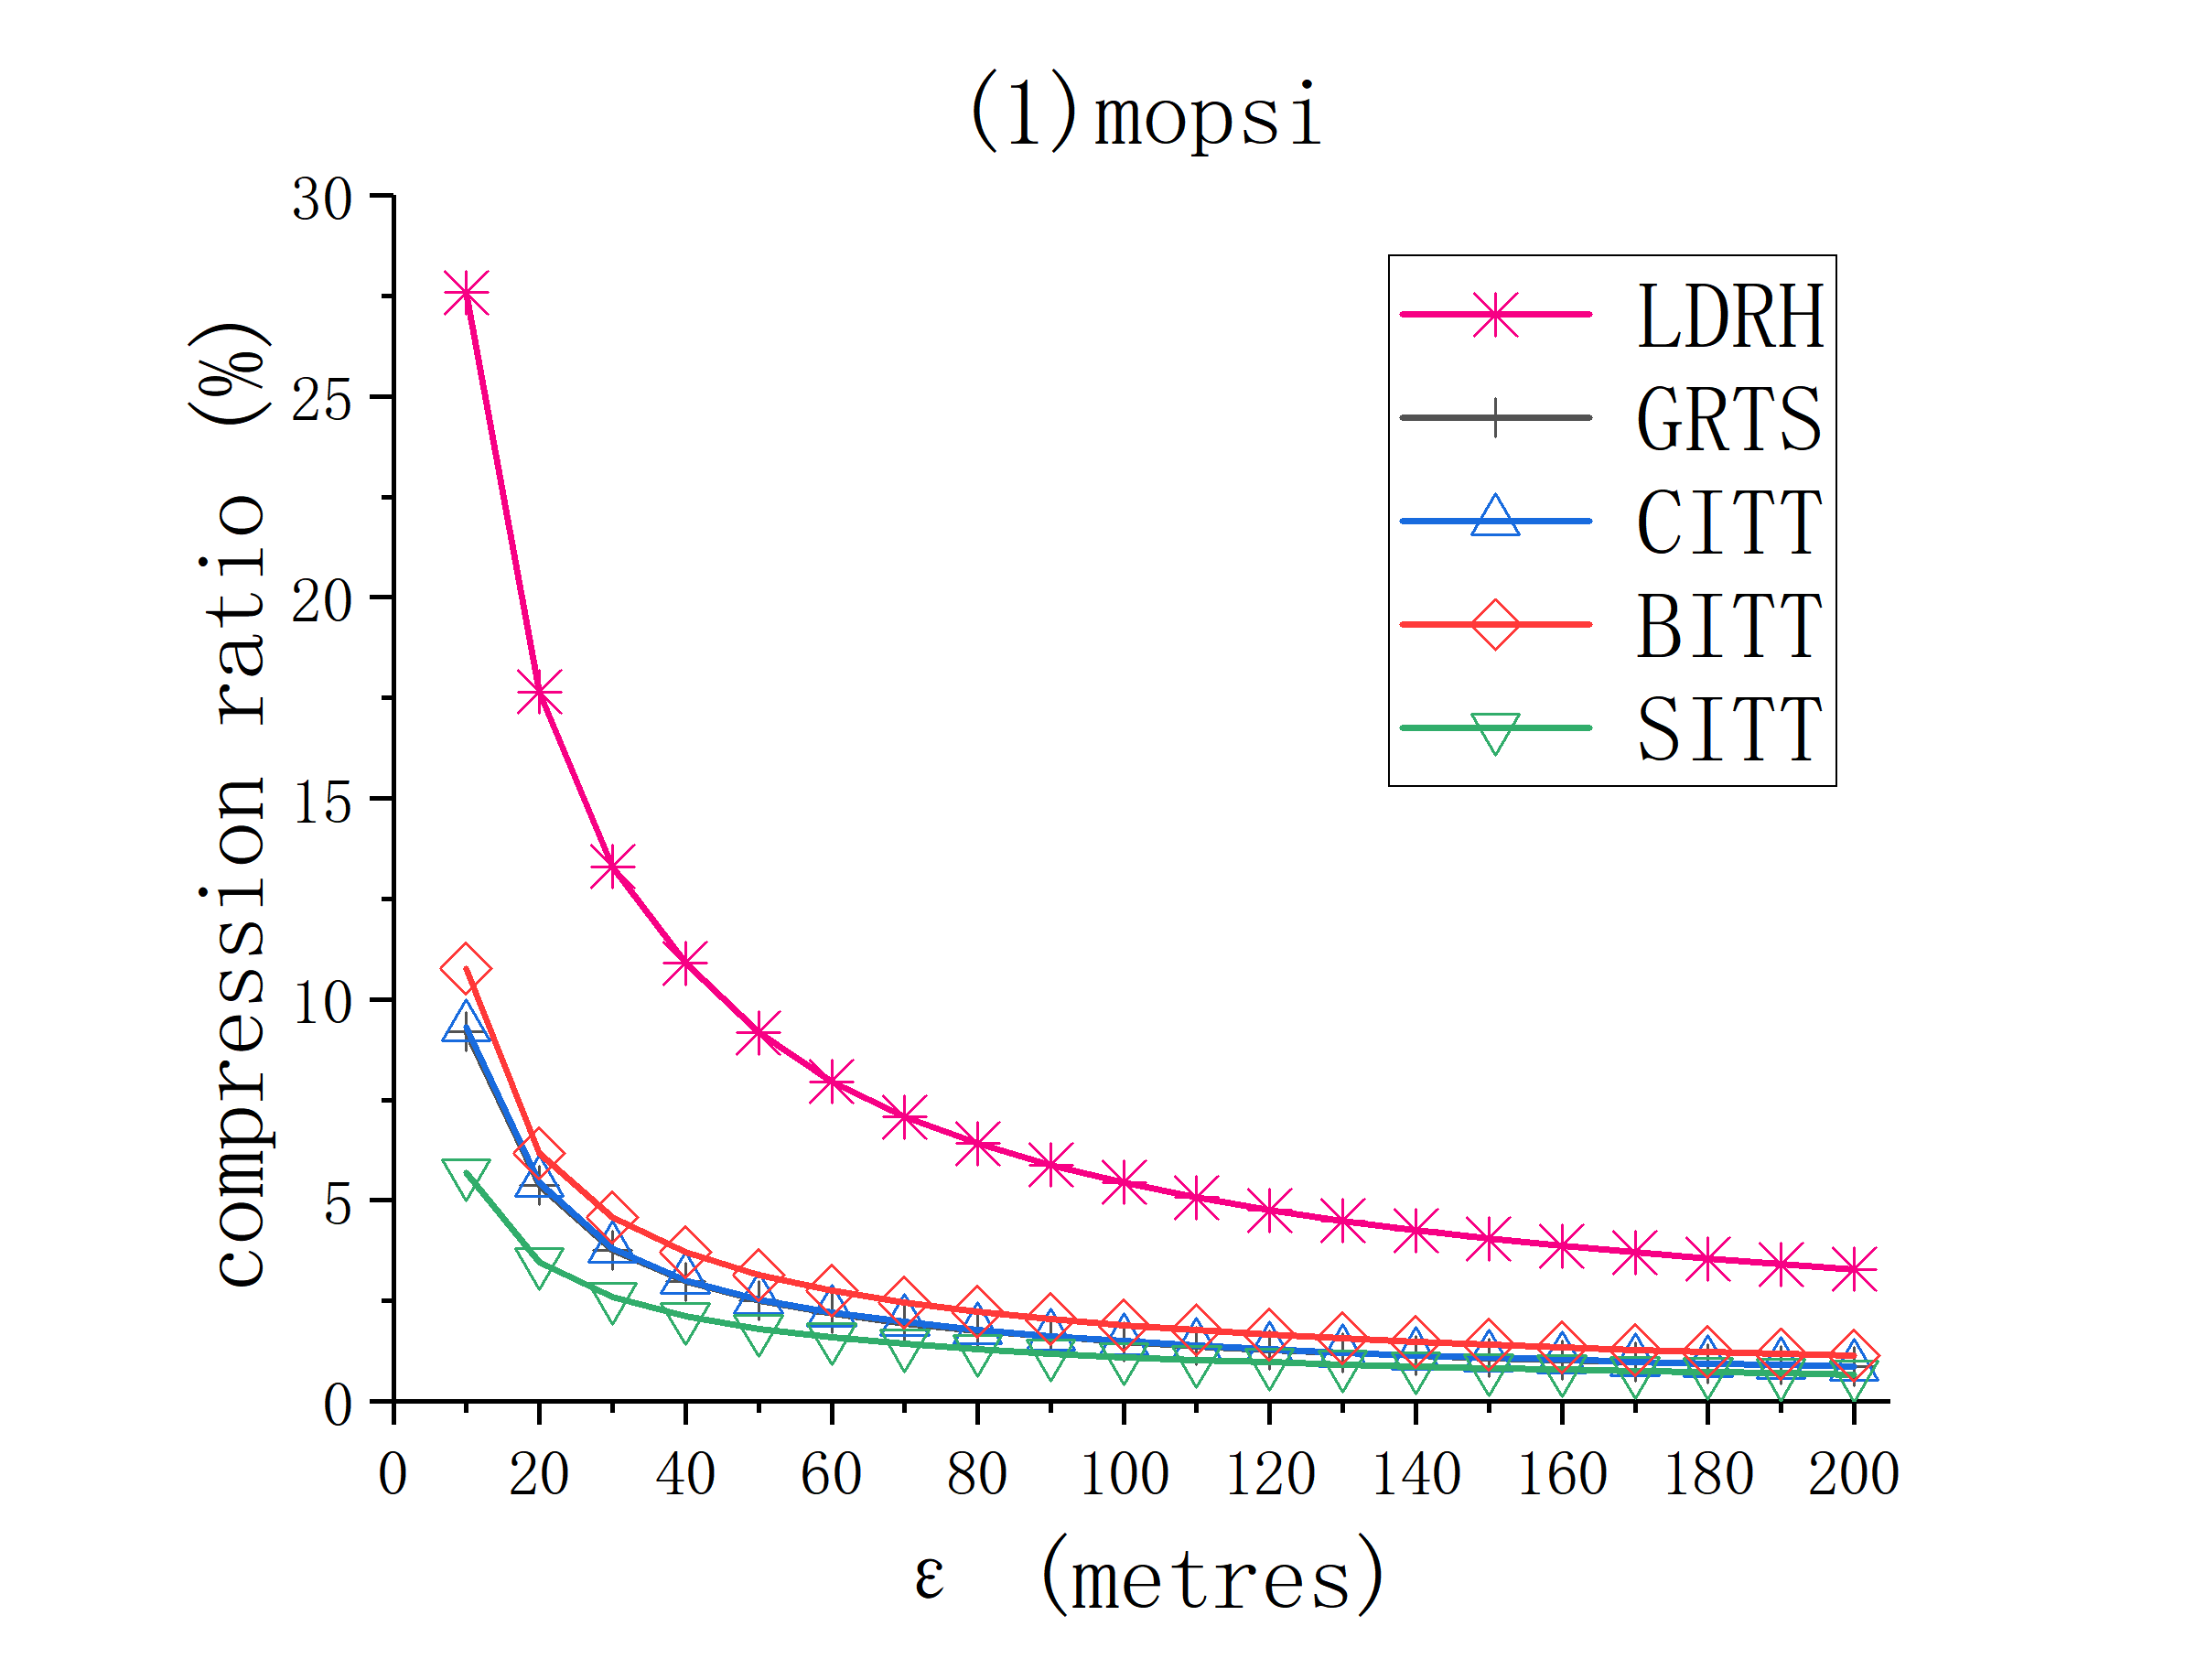
\includegraphics[scale = 0.580]{figures/Fig-mopsi-compression-ratio.png}\hspace{-1ex}
	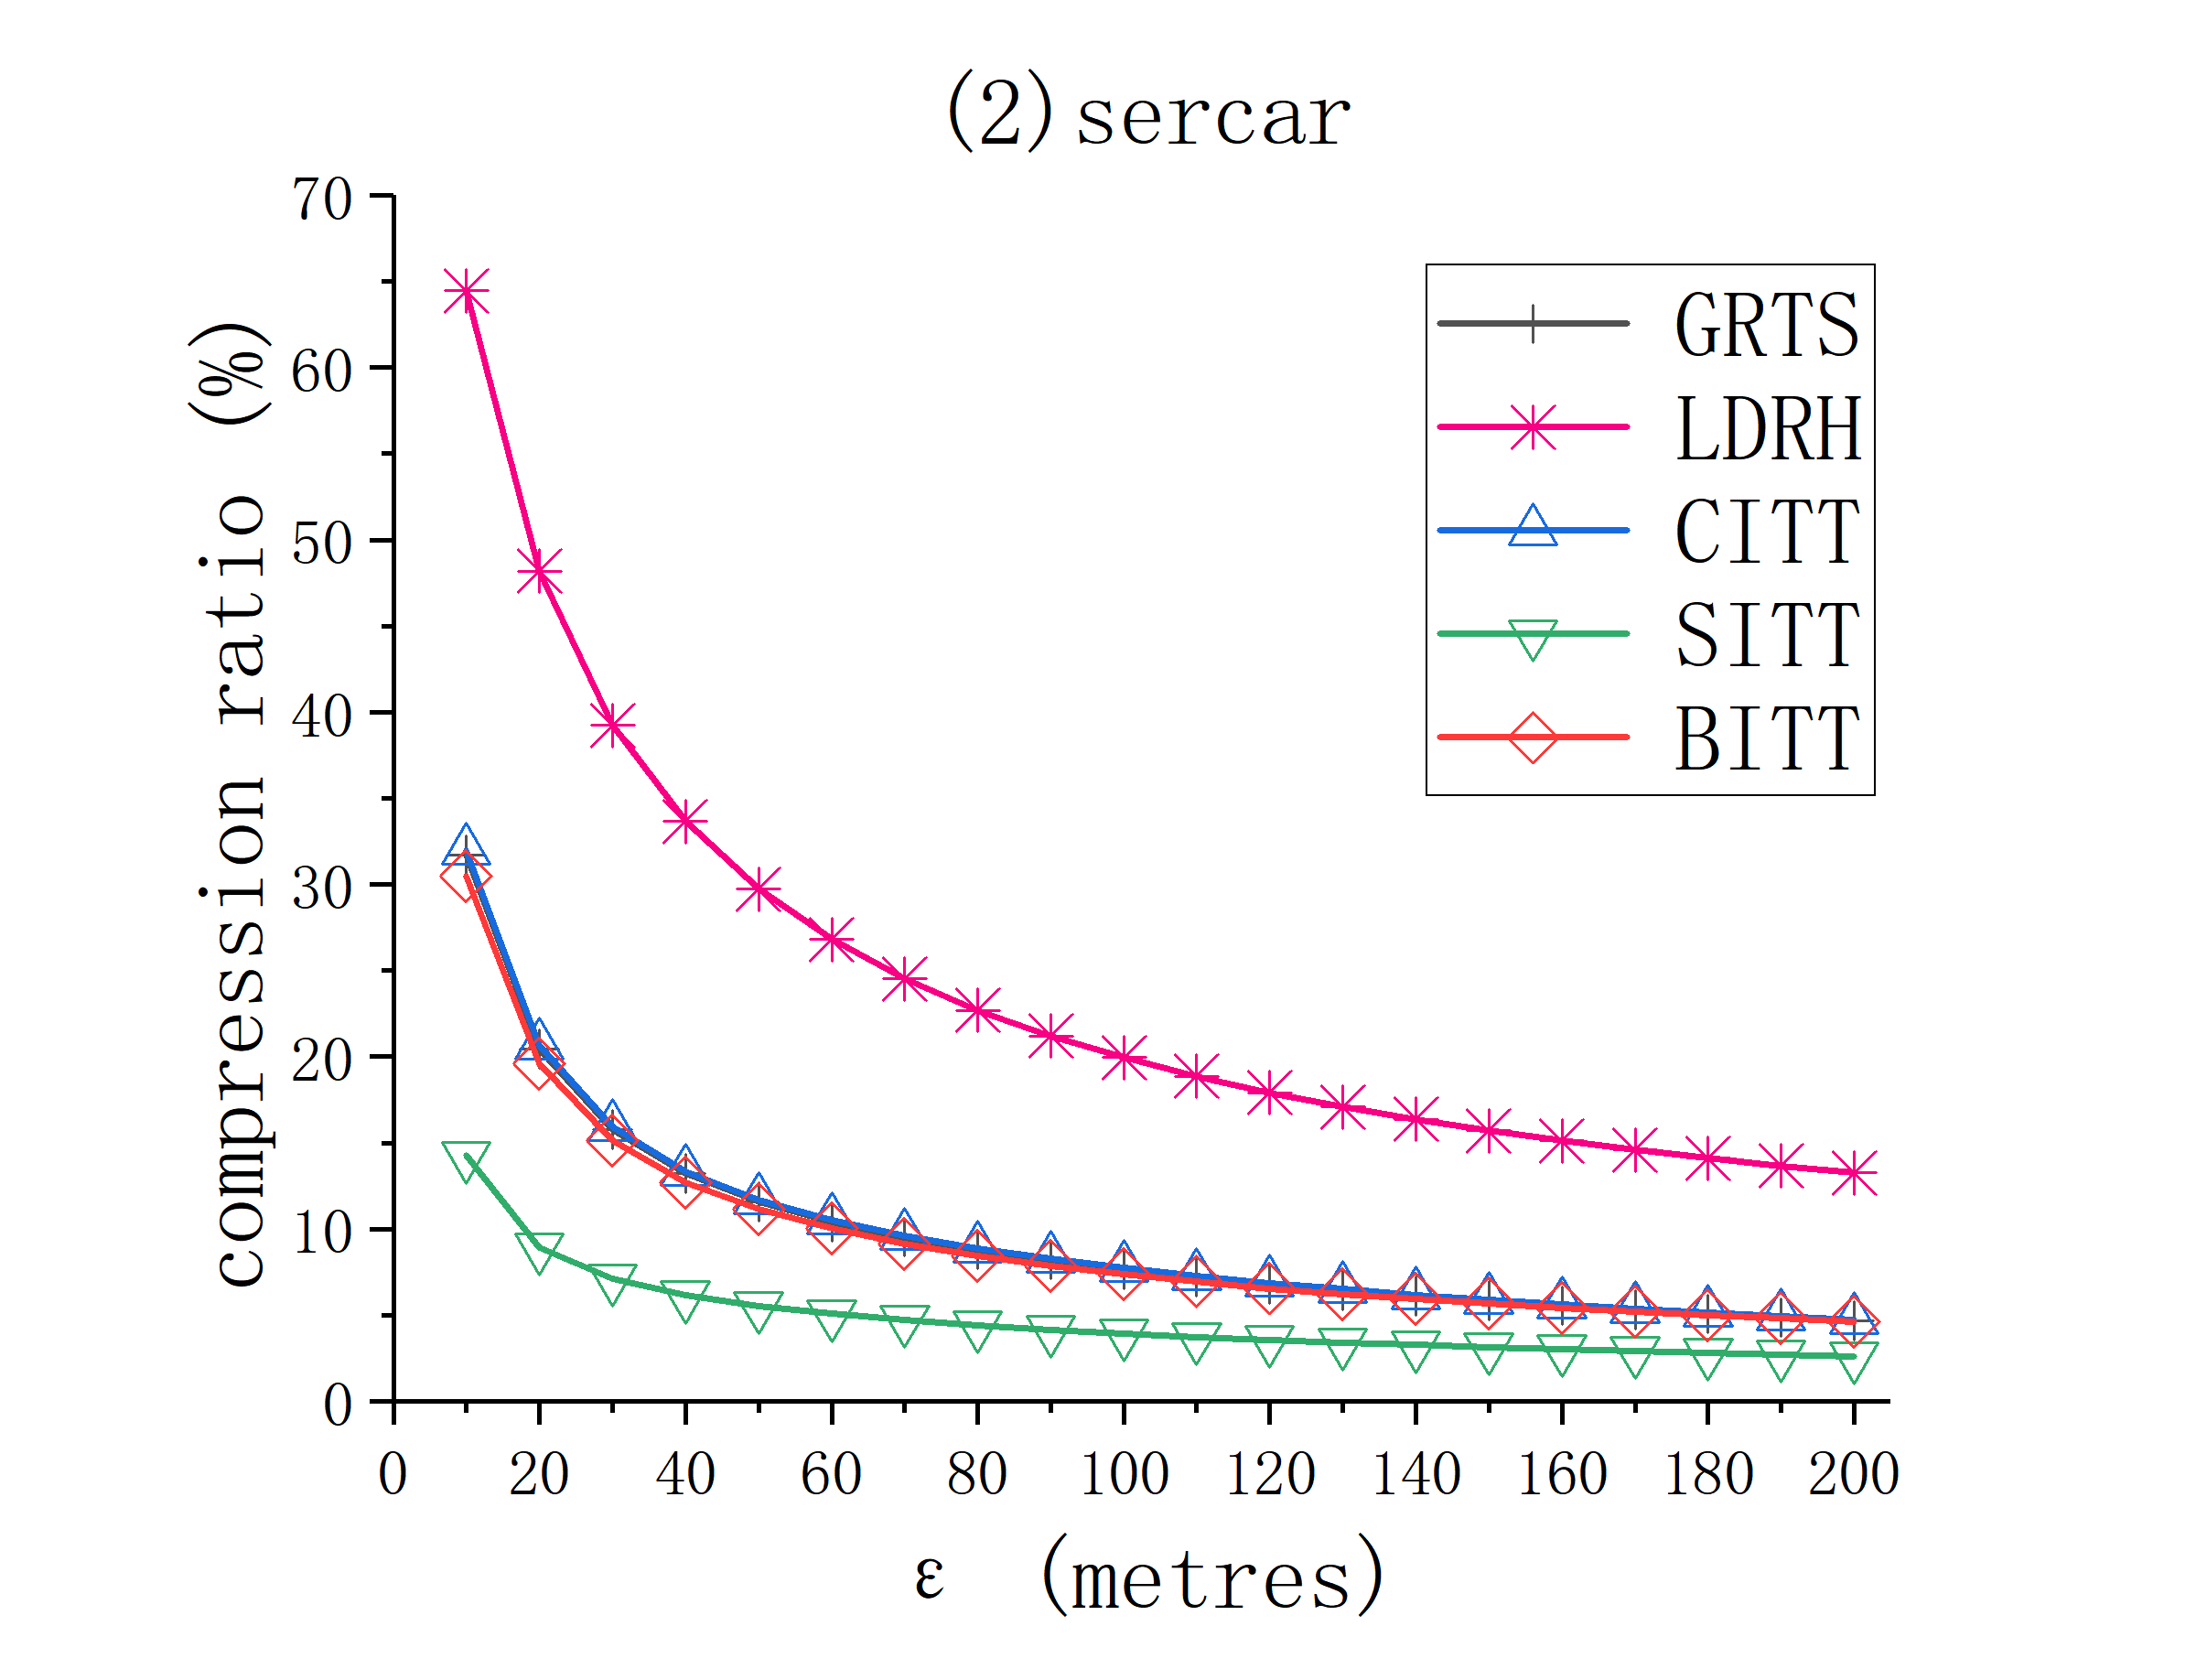
\includegraphics[scale = 0.580]{figures/Fig-sercar-compression-ratio.png}\hspace{-1ex}
	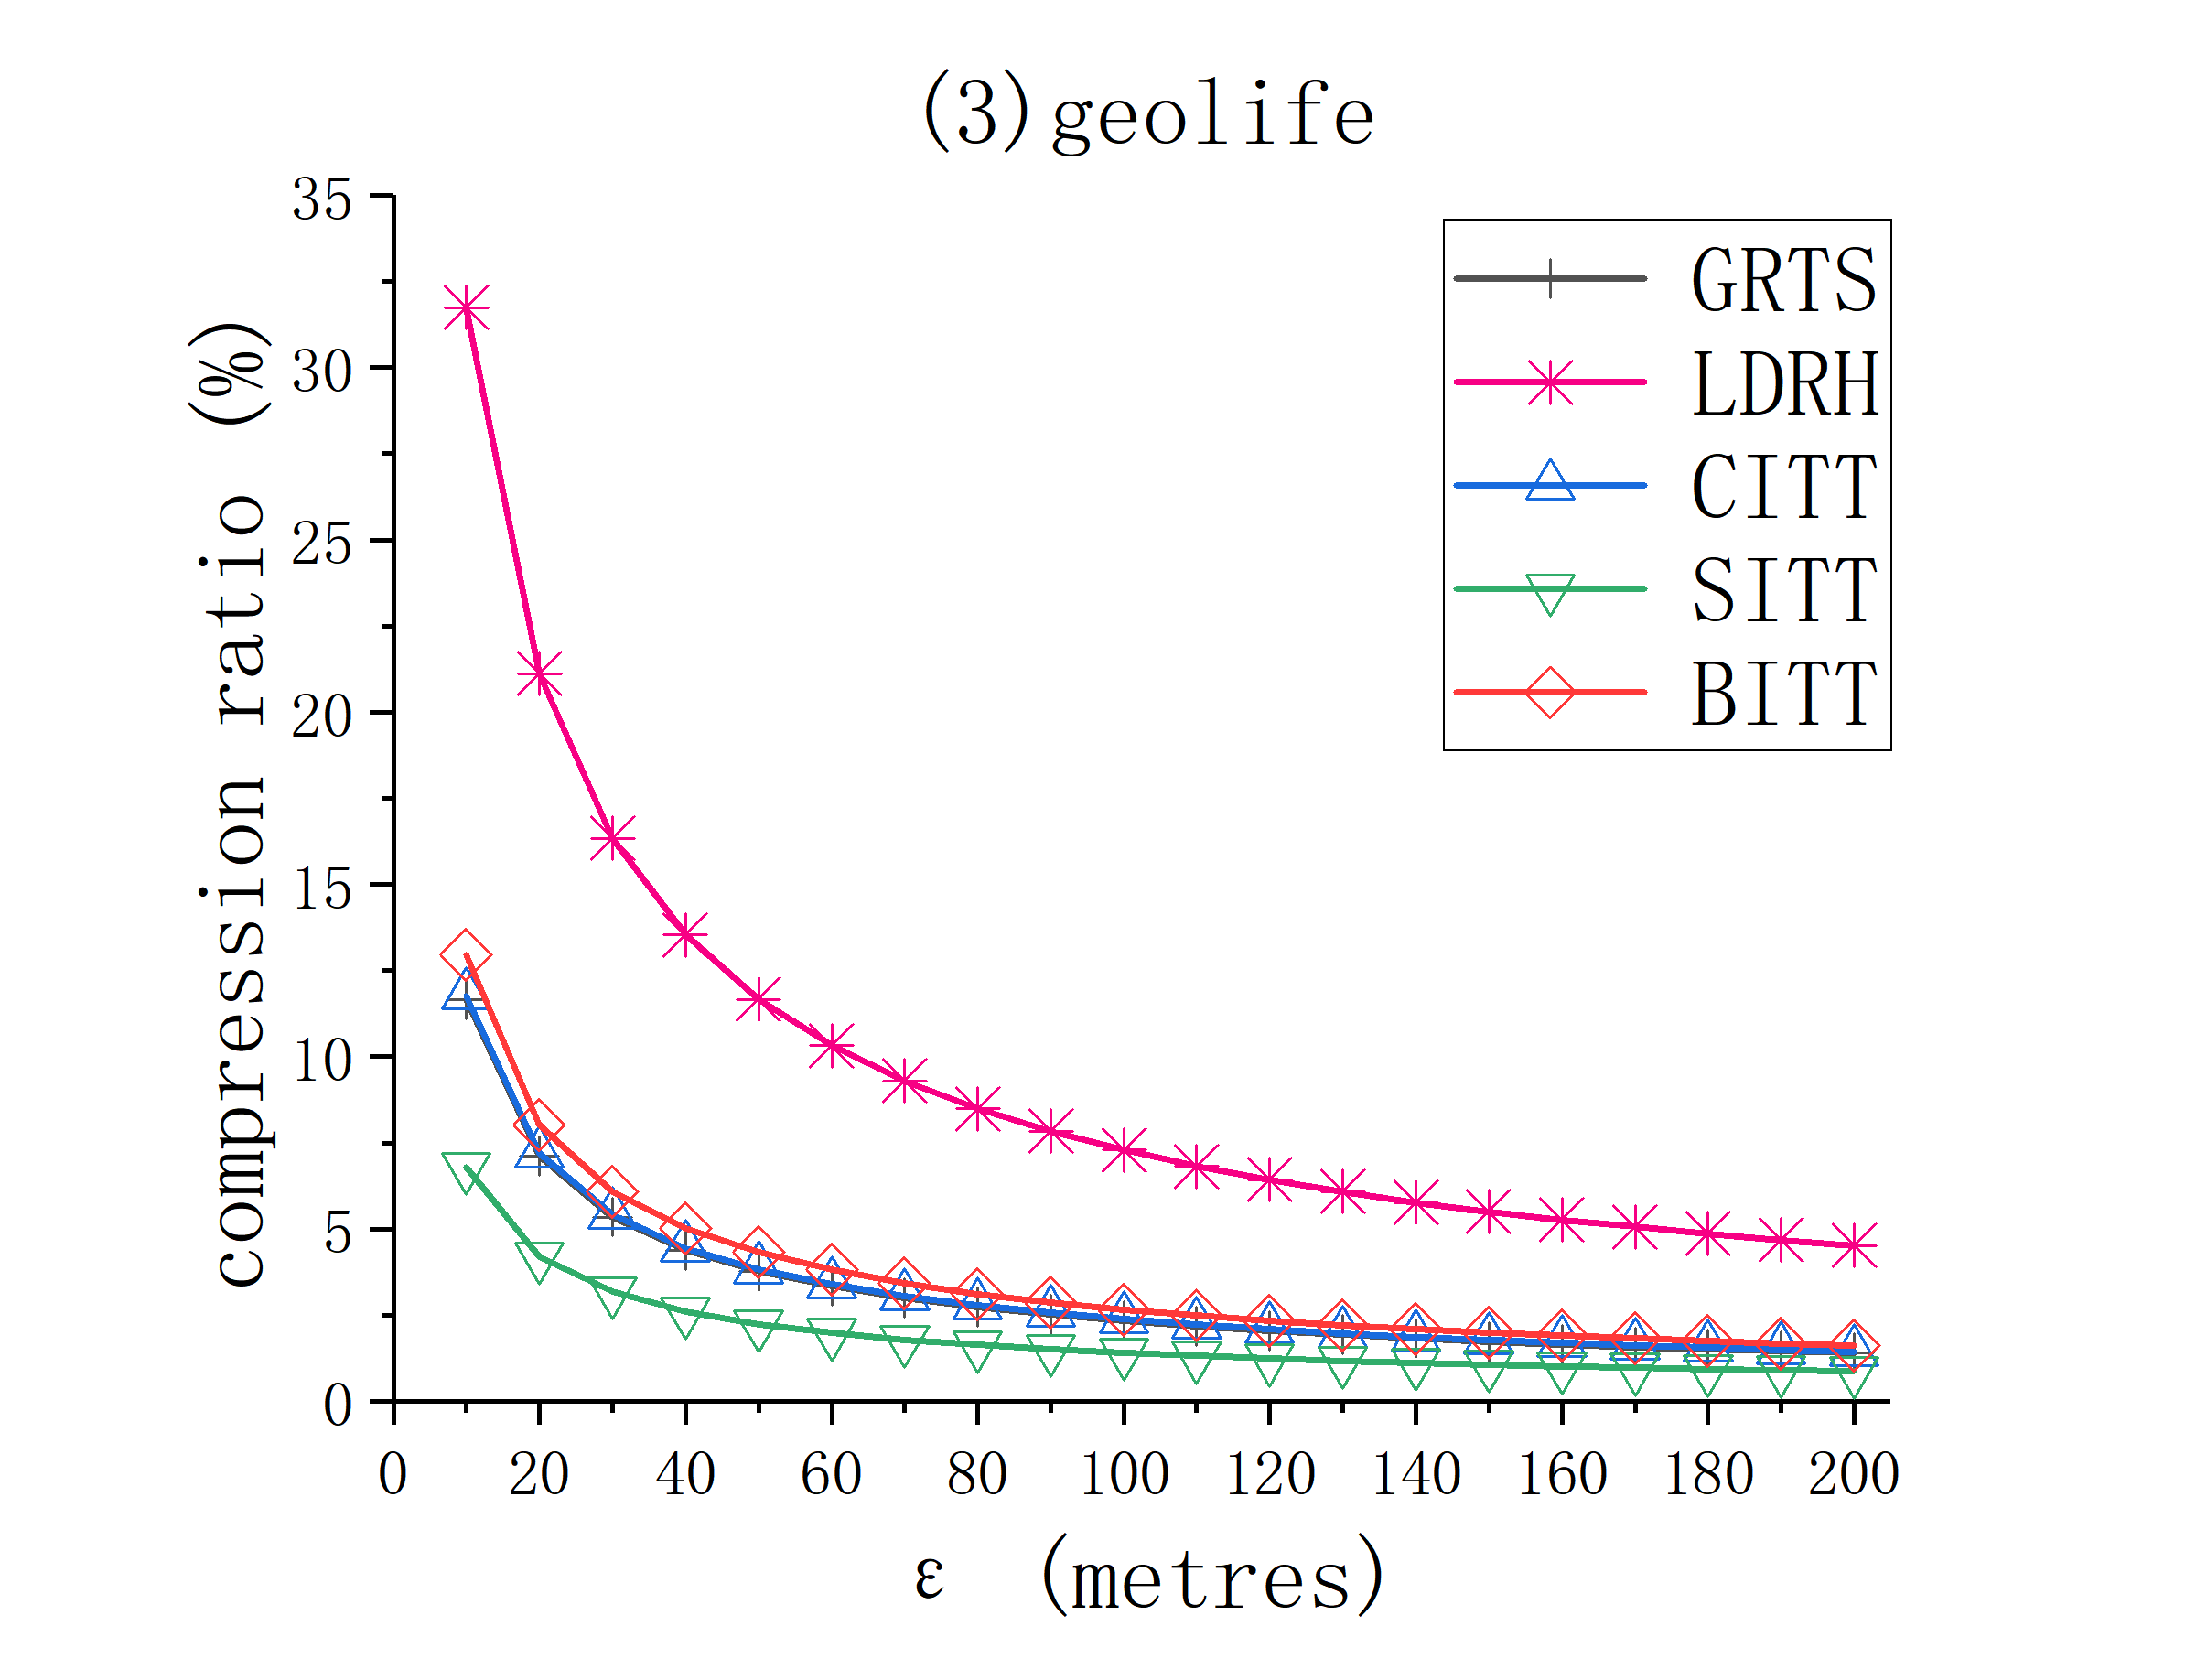
\includegraphics[scale = 0.580]{figures/Fig-geolife-compression-ratio.png}\hspace{0ex}
	\vspace{-1ex}
	\caption{\small Evaluation of compression ratios: varying error bounds $\epsilon_{sed}$ and $\epsilon_{ped}$.}
	\label{fig:compression-ratio}
	\vspace{-1ex}
\end{figure*}



\begin{figure*}[tb!]
	\centering
	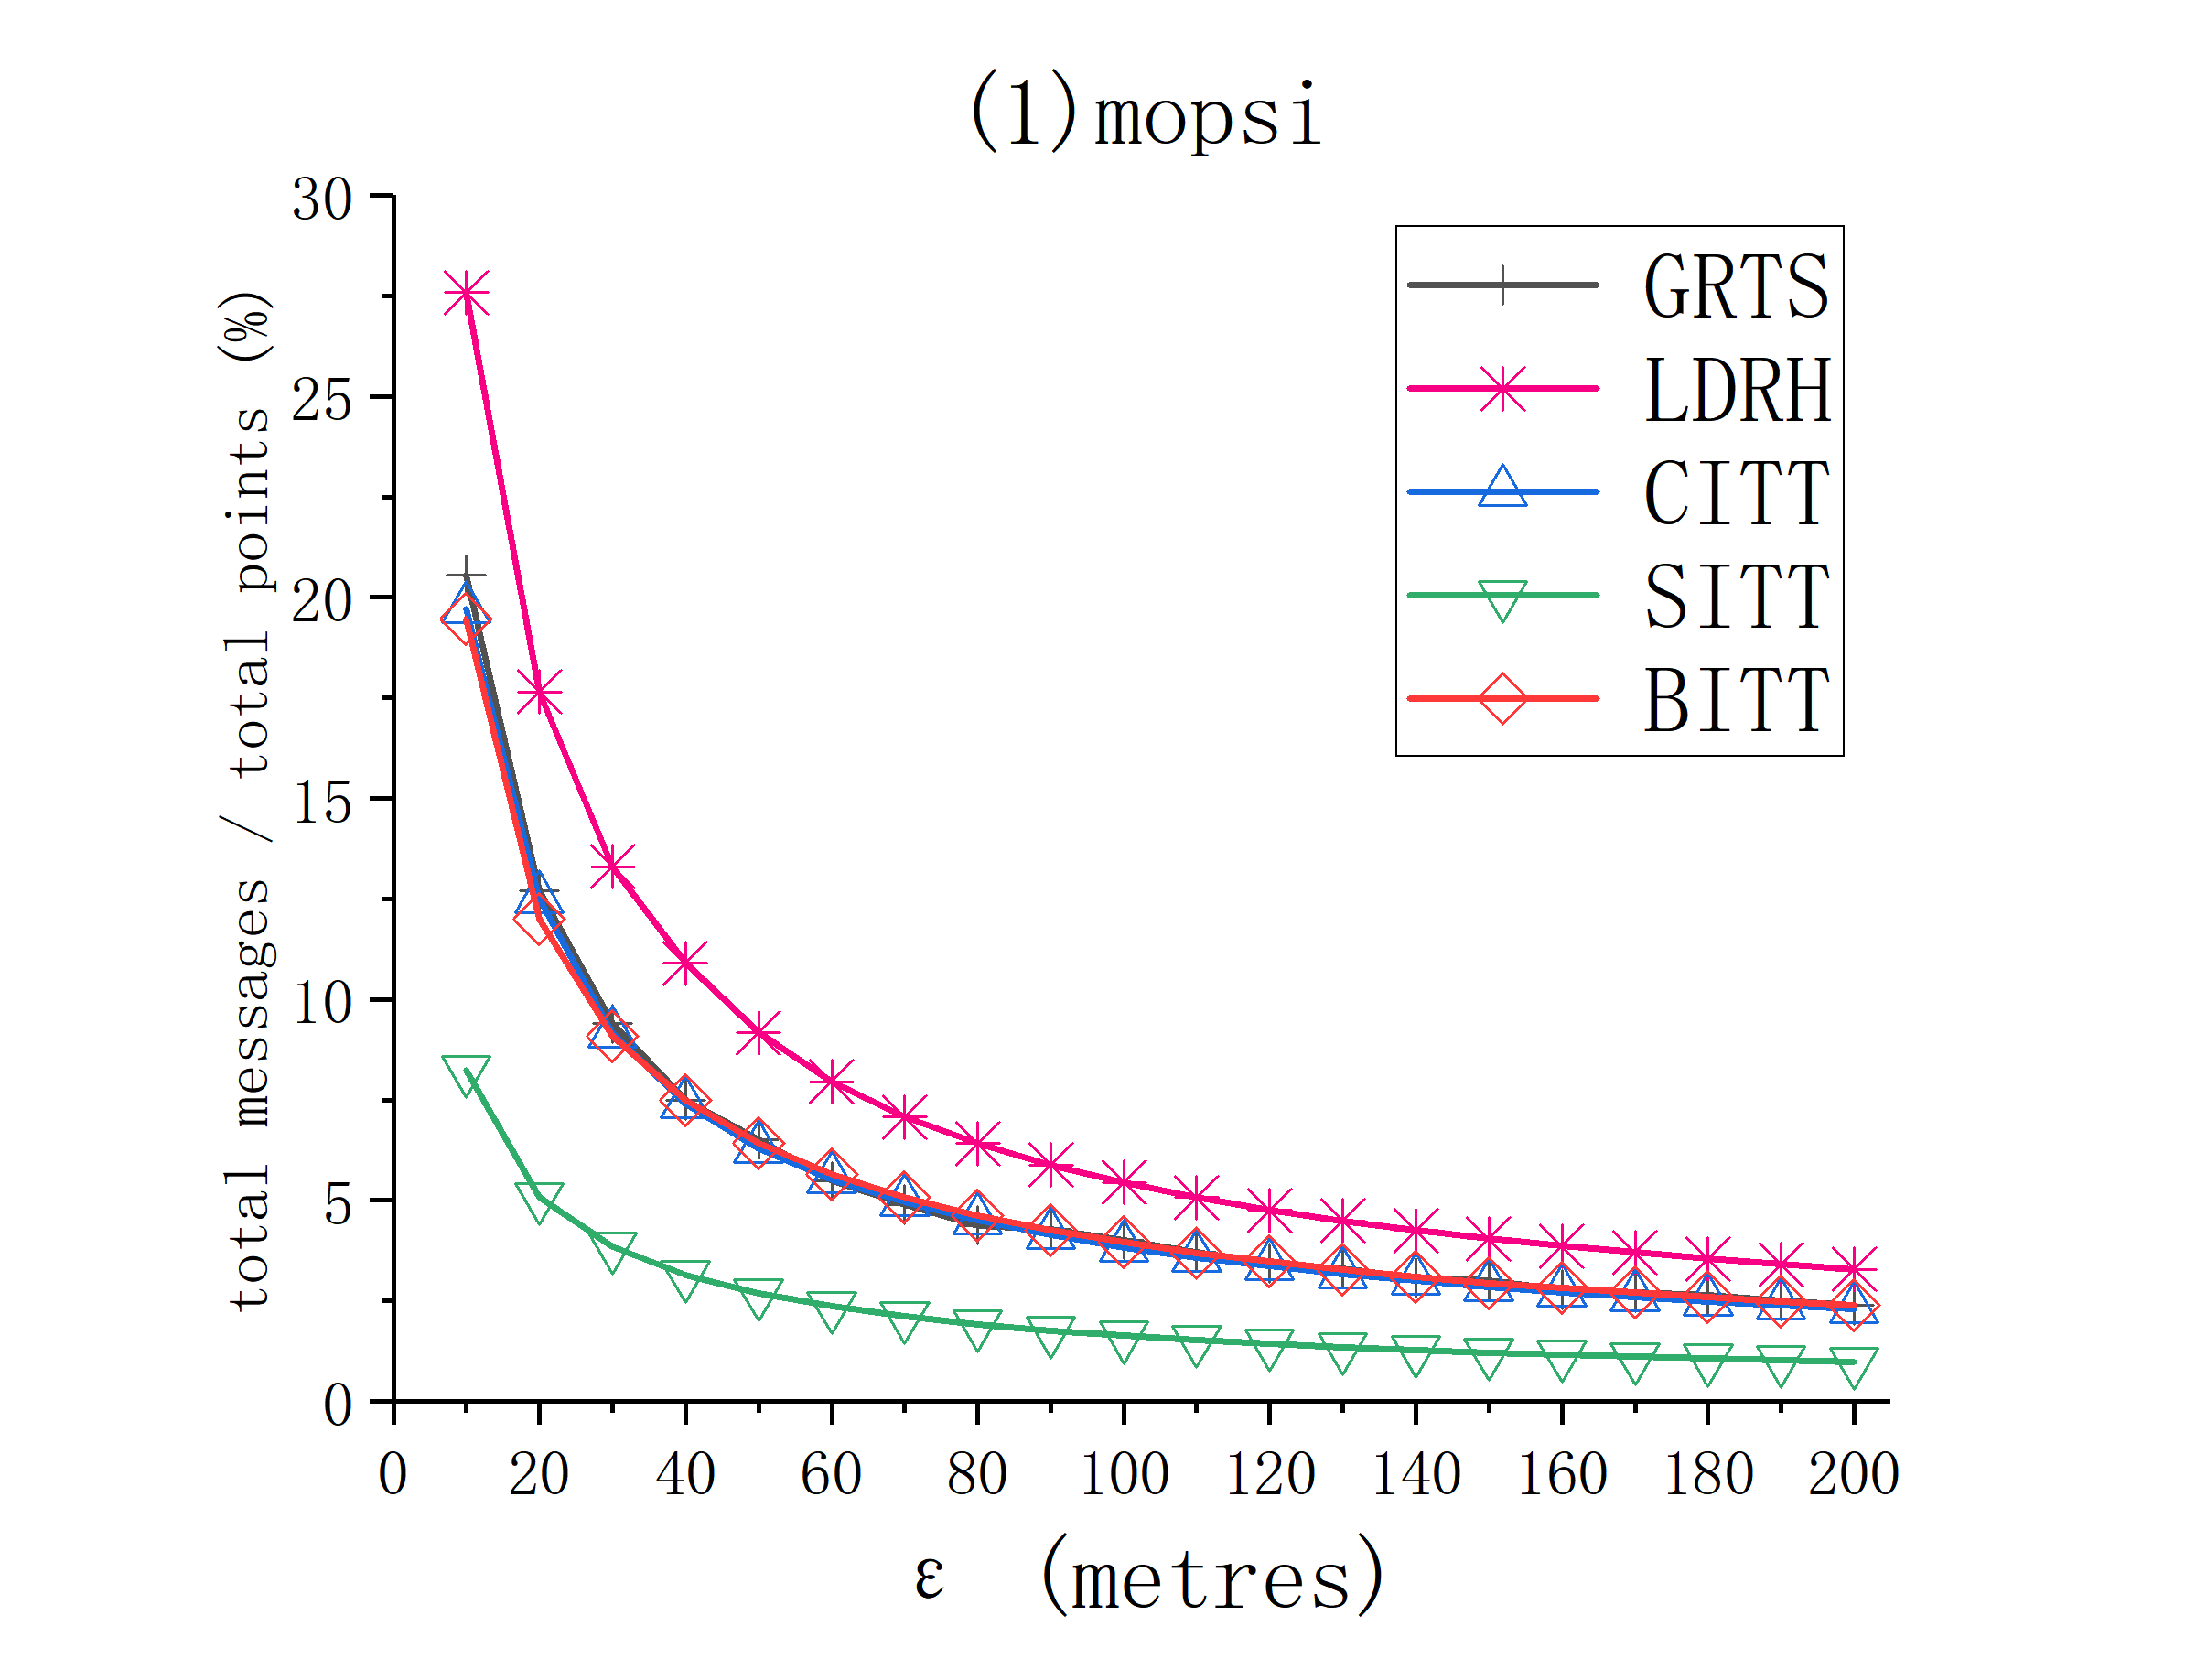
\includegraphics[scale = 0.580]{figures/Fig-mopsi-total-messages.png}\hspace{-1ex}
	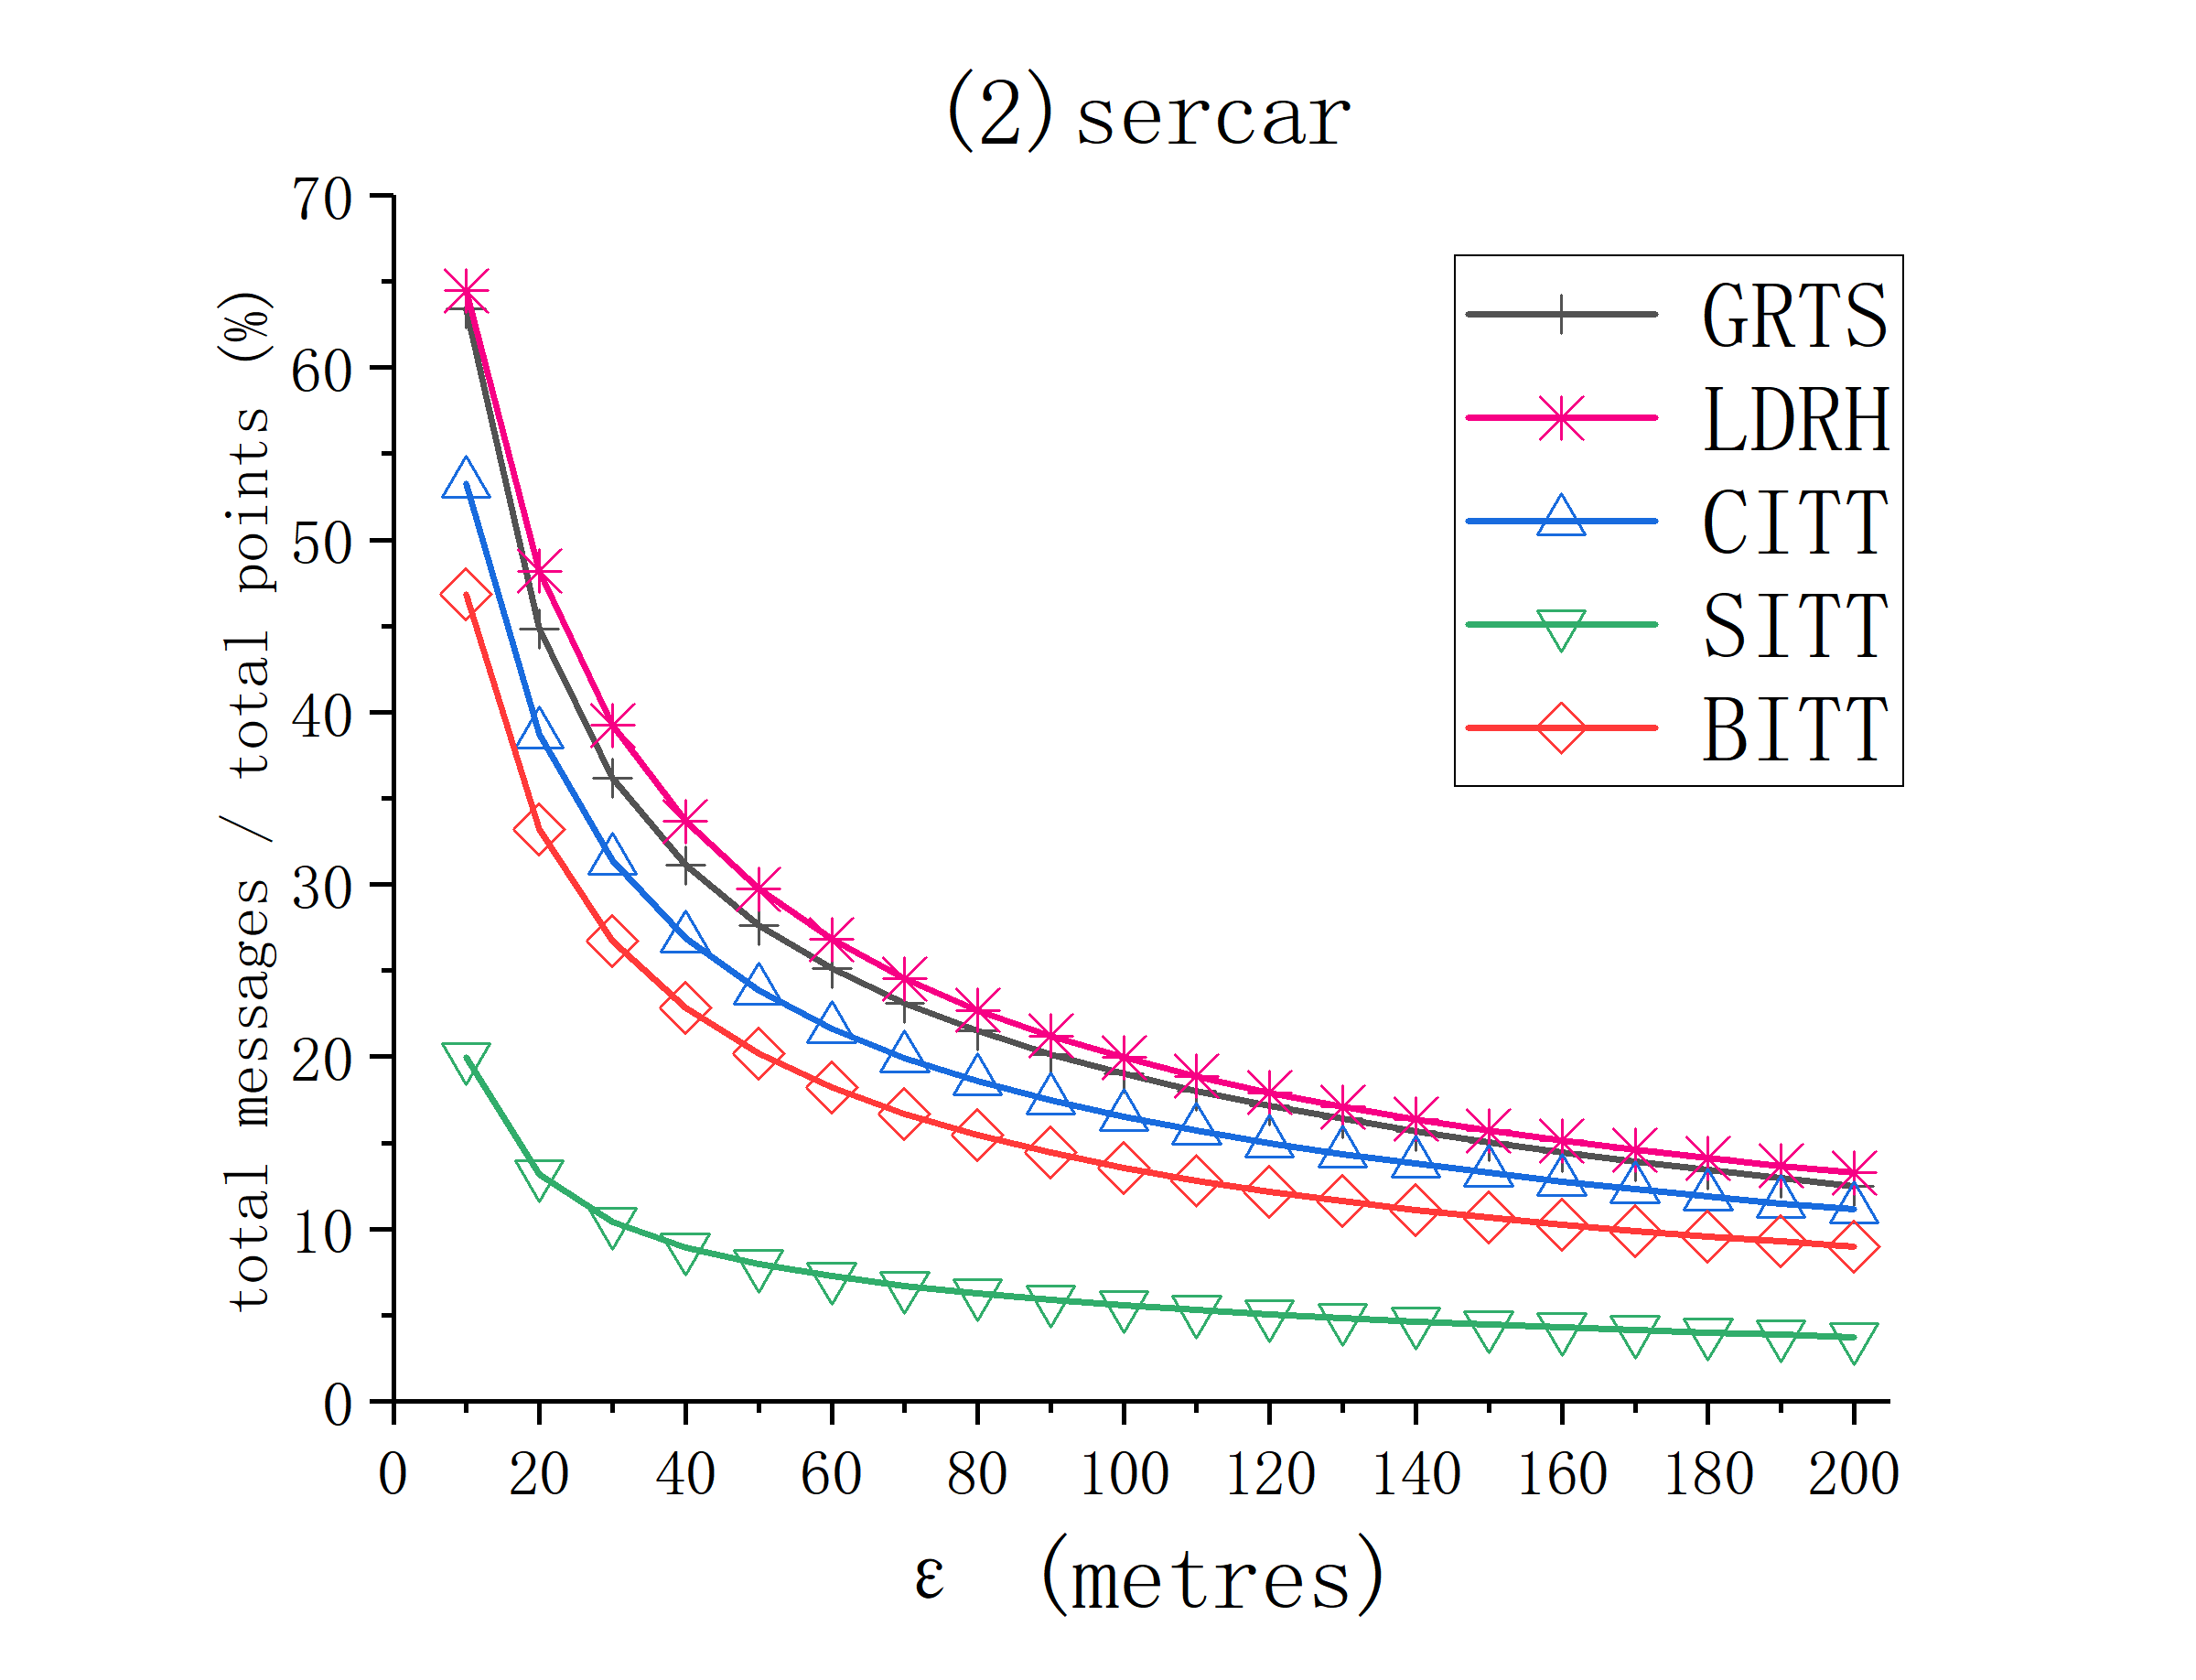
\includegraphics[scale = 0.580]{figures/Fig-sercar-total-messages.png}\hspace{-1ex}
	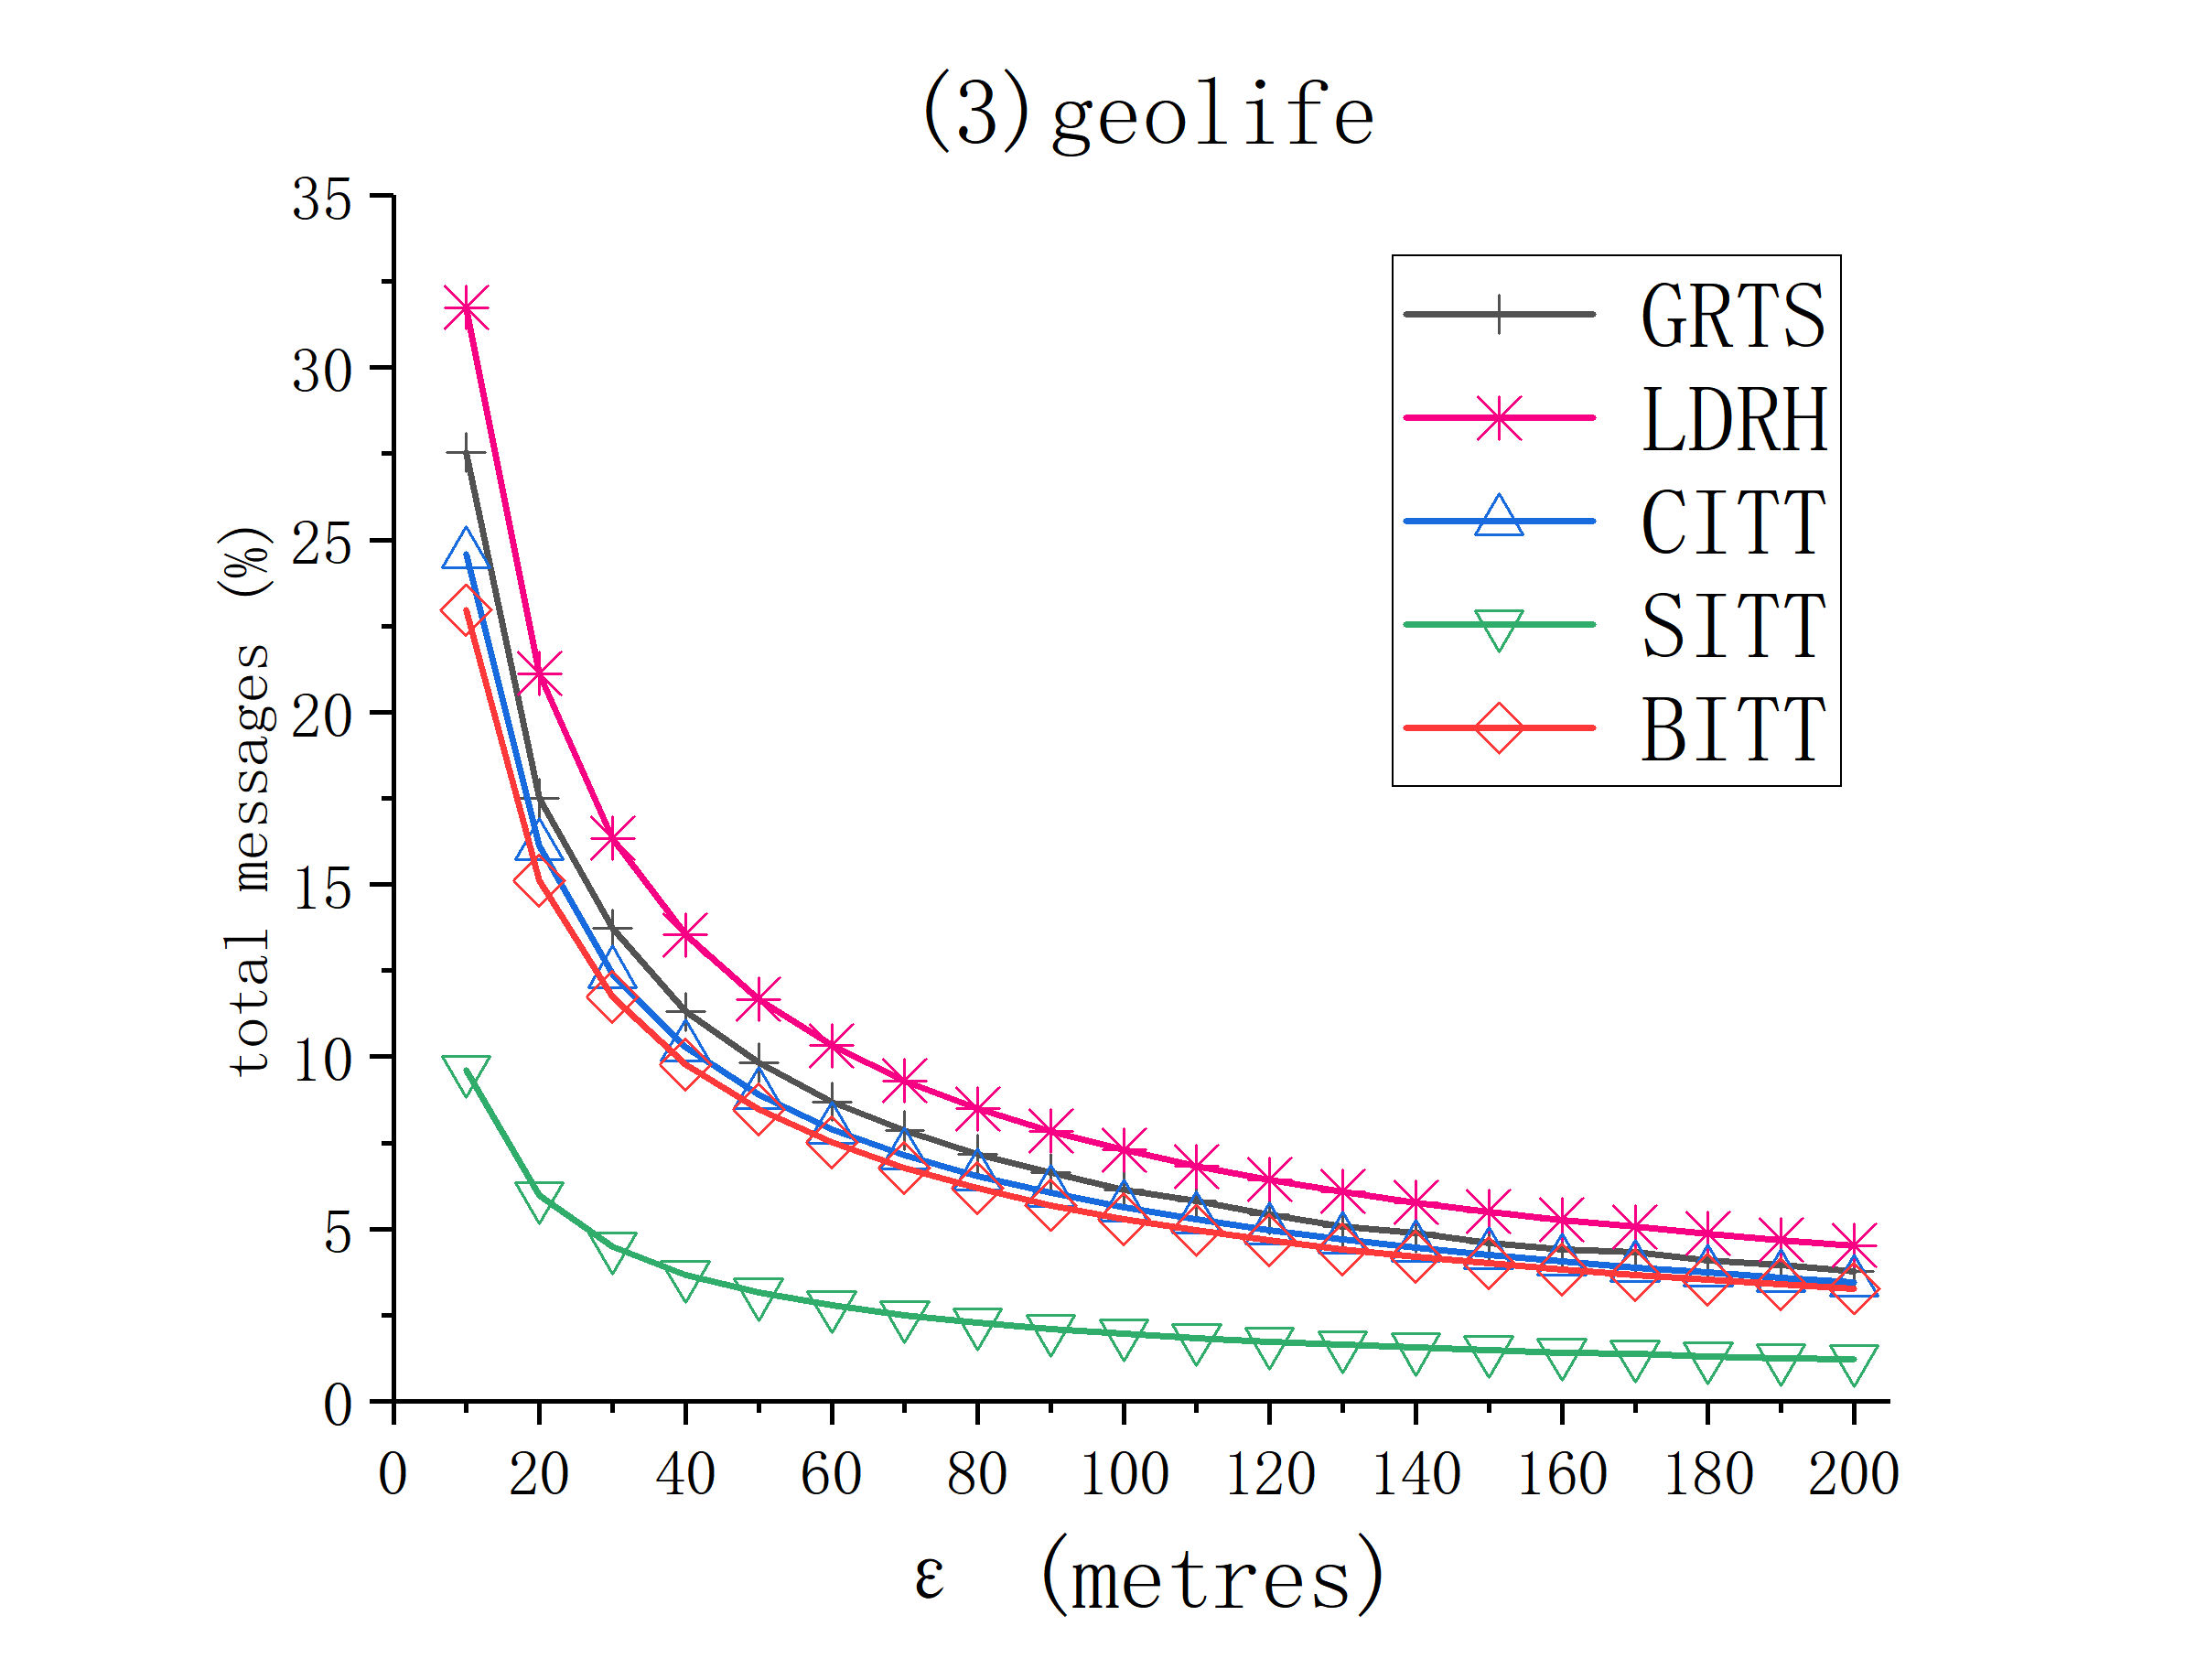
\includegraphics[scale = 0.580]{figures/Fig-geolife-total-messages.png}\hspace{0ex}
	\vspace{-1ex}
	\caption{\small Evaluation of total messages: varying error bounds $\epsilon_{sed}$ and $\epsilon_{ped}$.}
	\label{fig:total-message}
	\vspace{-1ex}
\end{figure*}

\eat{%%%%%%%%%%%%%%%%%%%%velocity messages
\begin{figure*}[tb!]
	\centering
	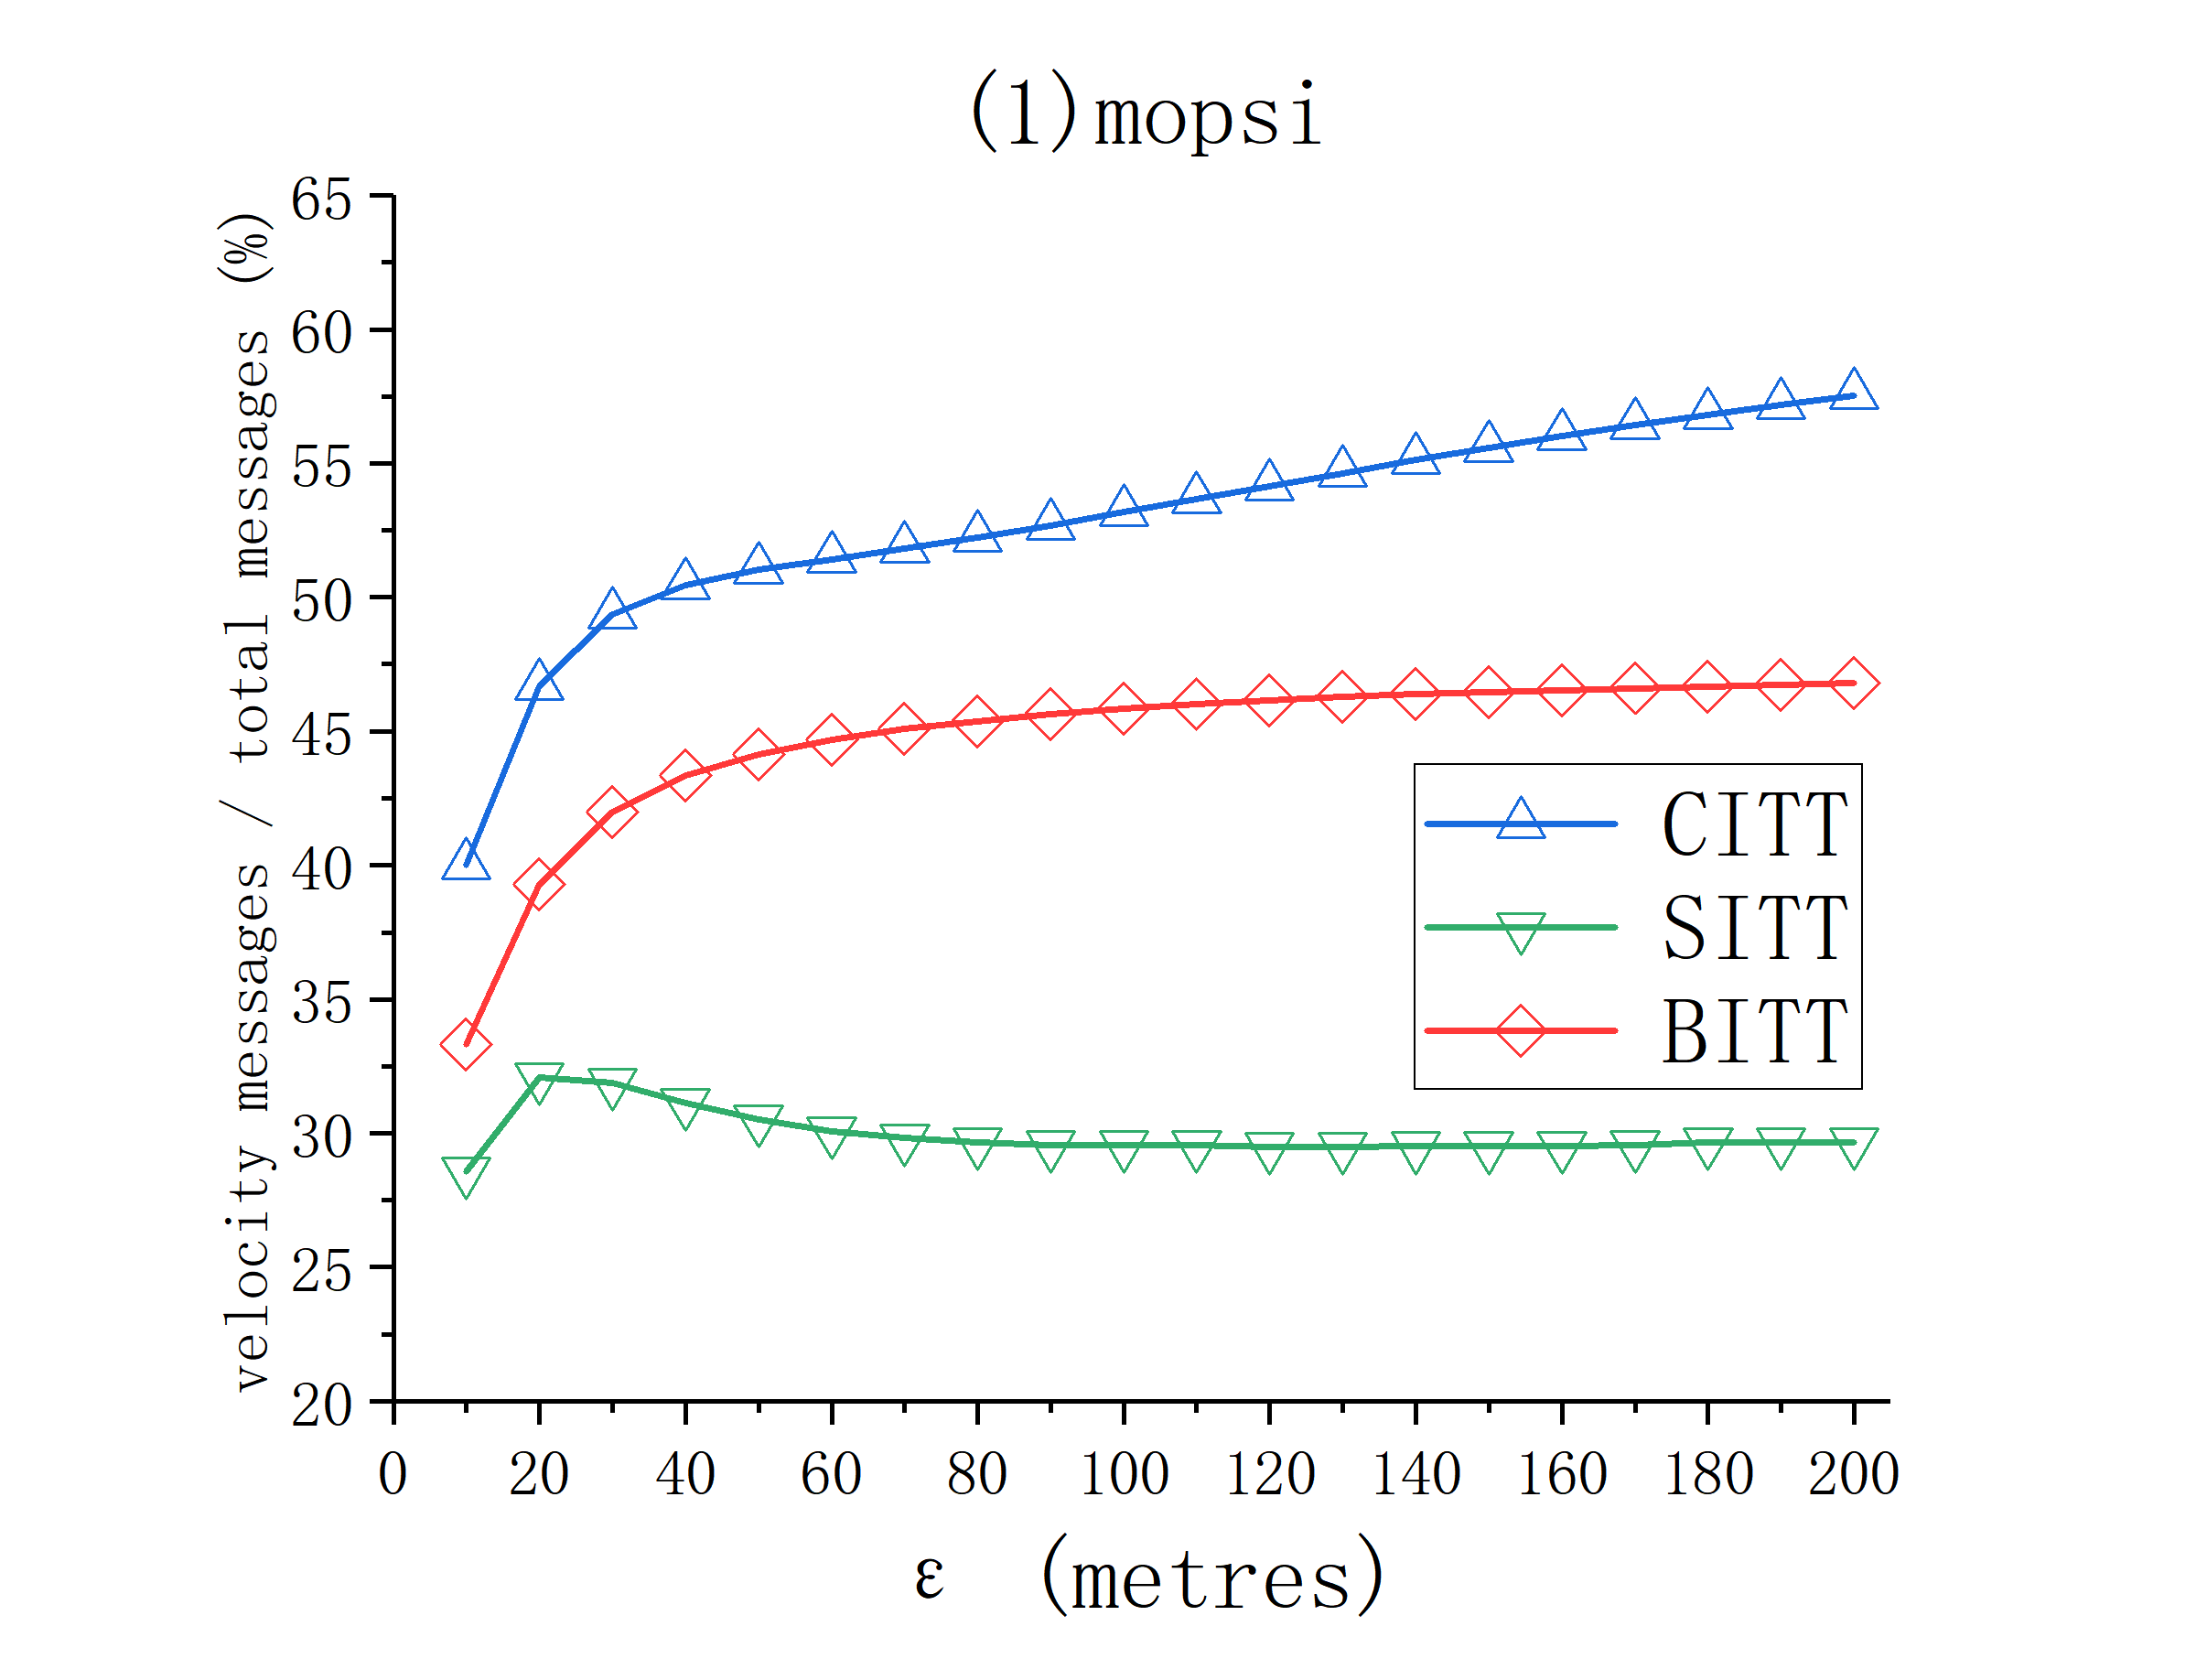
\includegraphics[scale = 0.580]{figures/Fig-mopsi-speed-messages.png}\hspace{-1ex}
	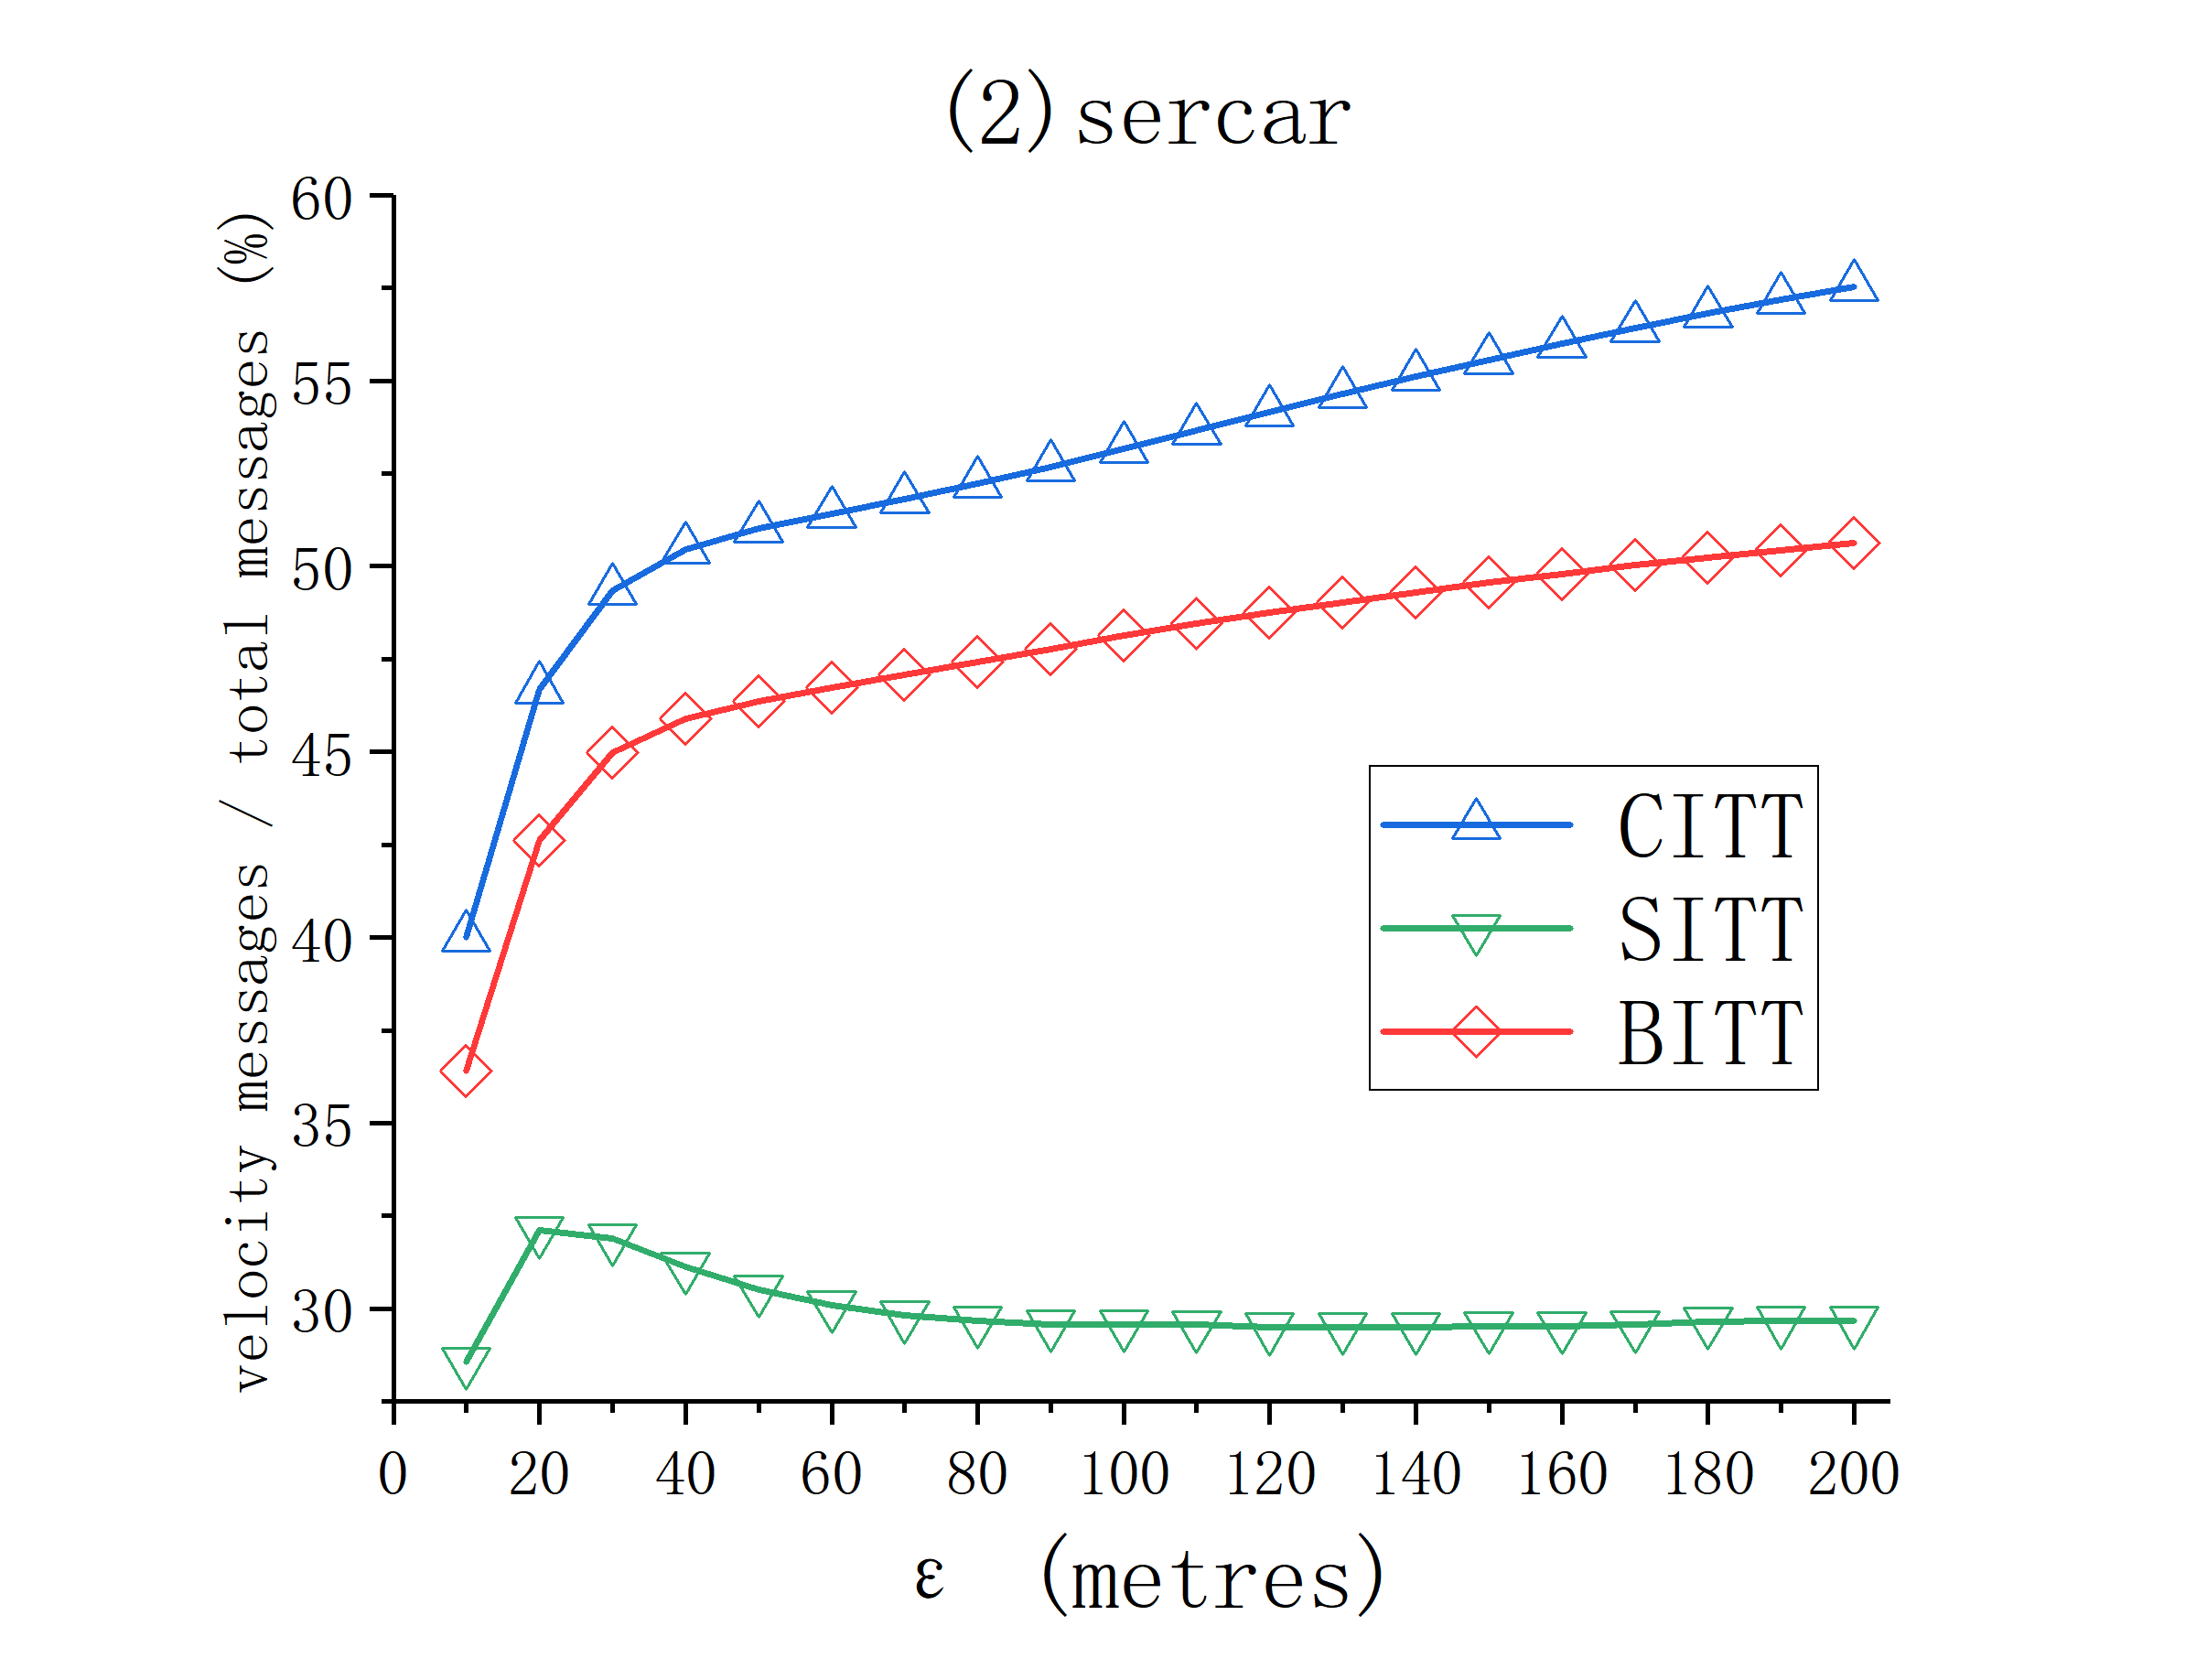
\includegraphics[scale = 0.580]{figures/Fig-sercar-speed-messages.png}\hspace{-1ex}
	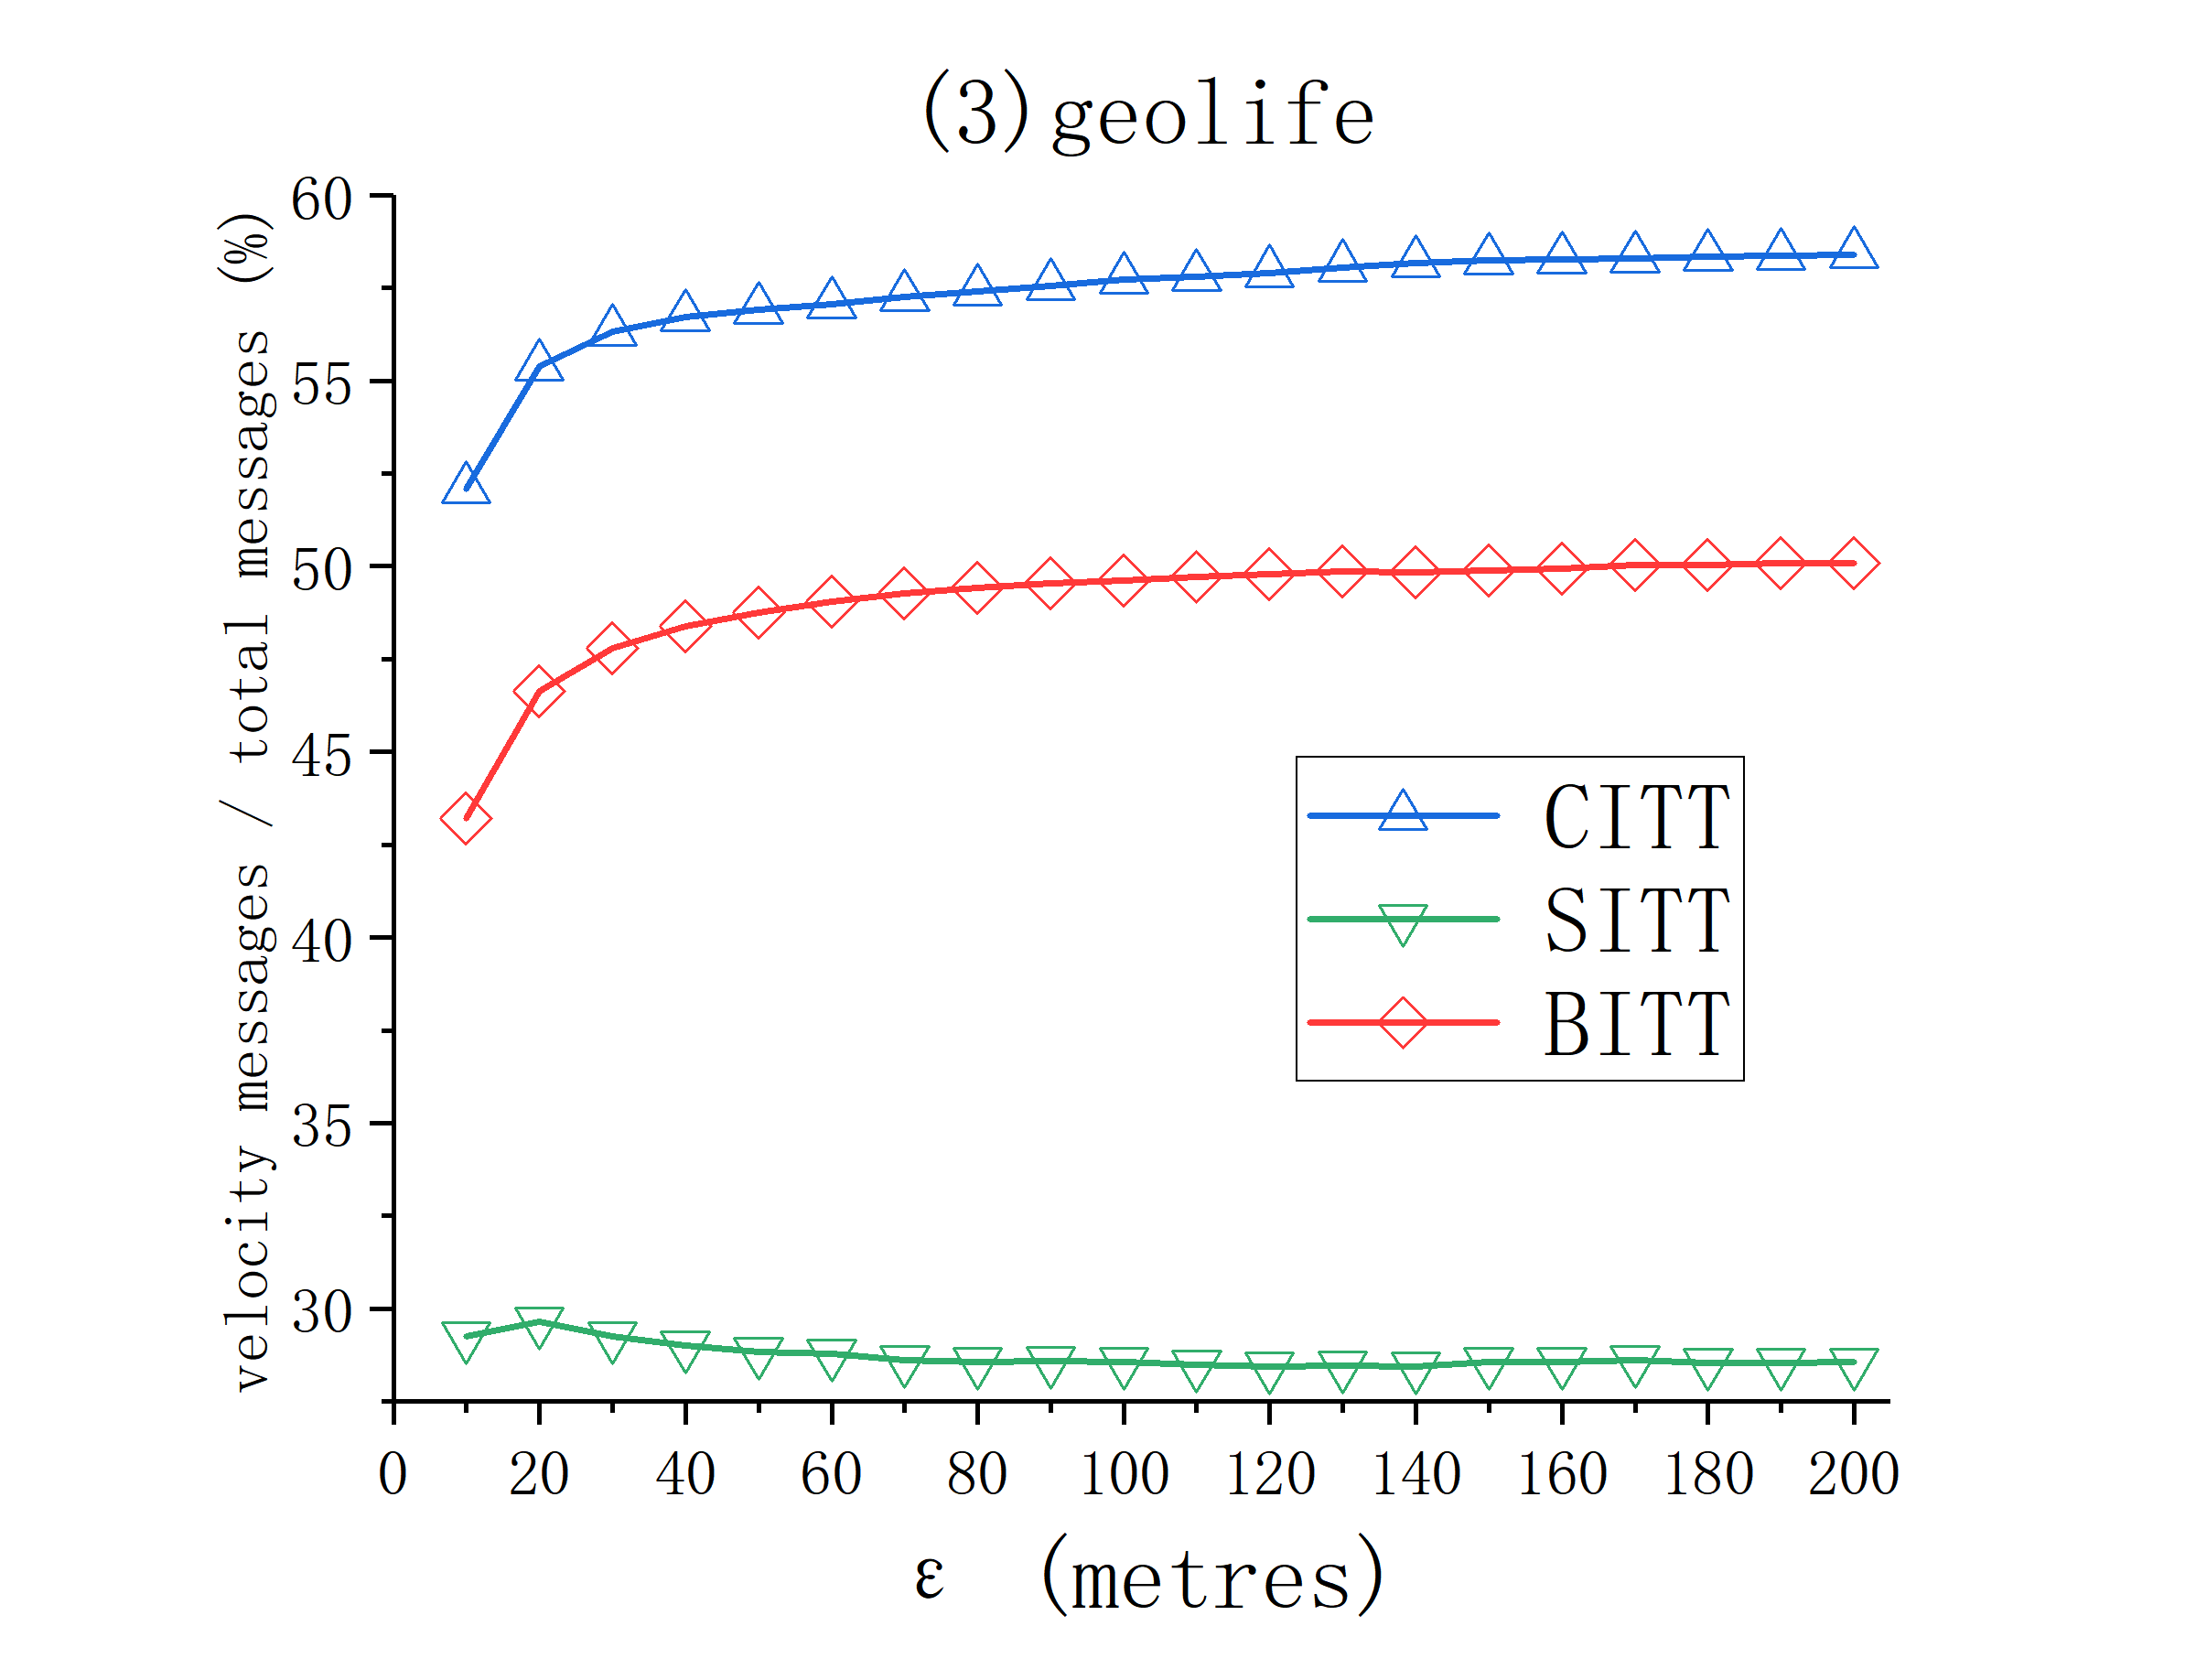
\includegraphics[scale = 0.580]{figures/Fig-geolife-speed-messages.png}\hspace{0ex}
	\vspace{-1ex}
	\caption{\small Evaluation of velocity messages: varying error bounds $\epsilon_{sed}$ and $\epsilon_{ped}$.}
	\label{fig:speed-message}
	\vspace{-1ex}
\end{figure*}
}%%%%%%%%%%%%%%%%%%%%%%velocity messages



\subsection{Experimental Results}

\subsubsection{Evaluation of~algorithm \bitt}
%%%%%%%%%%%% messages
This section test the impacts of \ped and \sed (\ie the shapes of finite beams) on algorithm \bitt. We varied error bounds $\epsilon_{sed}$ and $\epsilon_{ped}$ from $10$ meters to $200$ meters satisfying $\epsilon_{sed} \ge \epsilon_{ped}$ on the entire three datasets, respectively. The results are reported in Figures~\ref{fig:bitt-compression-ratio}, \ref{fig:bitt-total-message}, \ref{fig:bitt-sed-error} and \ref{fig:bitt-ped-error}.

%\stitle{Message and compression ratios}. Figures~\ref{fig:bitt-total-message} and \ref{fig:bitt-compression-ratio} tell 

\ni (1) Both message and compression ratios decrease with the increase of $\epsilon_{sed}$ and $\epsilon_{ped}$, respectively. It is clear that when the tracking area becomes larger, \bitt is more tolerant of the distance deviation of a moving object, hence, fewer messages are transmitted and fewer data points are saved.

\ni (2) The velocity  $\vv{v}$ (see Figures~\ref{alg:citt-s-full} and ~\ref{alg:bitt}) is not frequently updated during the process of a sub-trajectory for all $\epsilon$ in all datasets. More specifically, a) when $\epsilon_{ped} \ge \epsilon_{sed}$, \ie~\bitt falls back to \citt, the \emph{position-velocity-messages} are on average $(39.59\%, 42.69\%, 47.20\%)$ of the total messages \wrt datasets (\mopsi, \sercar, \geolife), respectively, and b) when $\epsilon_{ped} << \epsilon_{sed}$, \ie~\bitt falls back to \sitt, the \emph{position-velocity-messages} are on average $(66.09\%, 71.29\%, 70.07\%)$ of the total messages \wrt datasets (\mopsi, \sercar, \geolife), respectively. Otherwise, \bitt has the number of \emph{position-velocity-messages} between \citt and \sitt.
%More than \myred{half} messages are \emph{position-velocity-messages}  for all $\epsilon$ in all datasets, meaning that, given a start point $P_s$ and an initial velocity $\vv{v}$ as the way shown in Figures~\ref{alg:citt-s-full} and ~\ref{alg:bitt}, 

%\ni (3) Dataset \sercar has the highest message and compression ratios, compared with datasets \mopsi and \geolife, due to its lowest sampling rate. 

\ni (3) Both average \ped and \sed errors increase with the increase of $\epsilon_{sed}$ and $\epsilon_{ped}$, respectively.

\ni (4) Given a $\epsilon_{sed}$, both the compression and message ratios, and the average \sed and \ped errors are constant for all $\epsilon_{ped}$ that are greater than $\epsilon_{sed}$, \eg $\epsilon_{sed}=10$ and $\epsilon_{ped} \ge 10$, showing that \bitt falls back to \citt in these cases.

%\ni (6) When $\epsilon_{sed} > \epsilon_{ped}$, the performance of algorithm \bitt will be similar to that of \sitt, as a result, the average \ped error will be much smaller than $\epsilon_{sed}$,
%the $\epsilon_{ped}$ is mainly in effect,

\begin{figure*}[tb!]
	\centering
	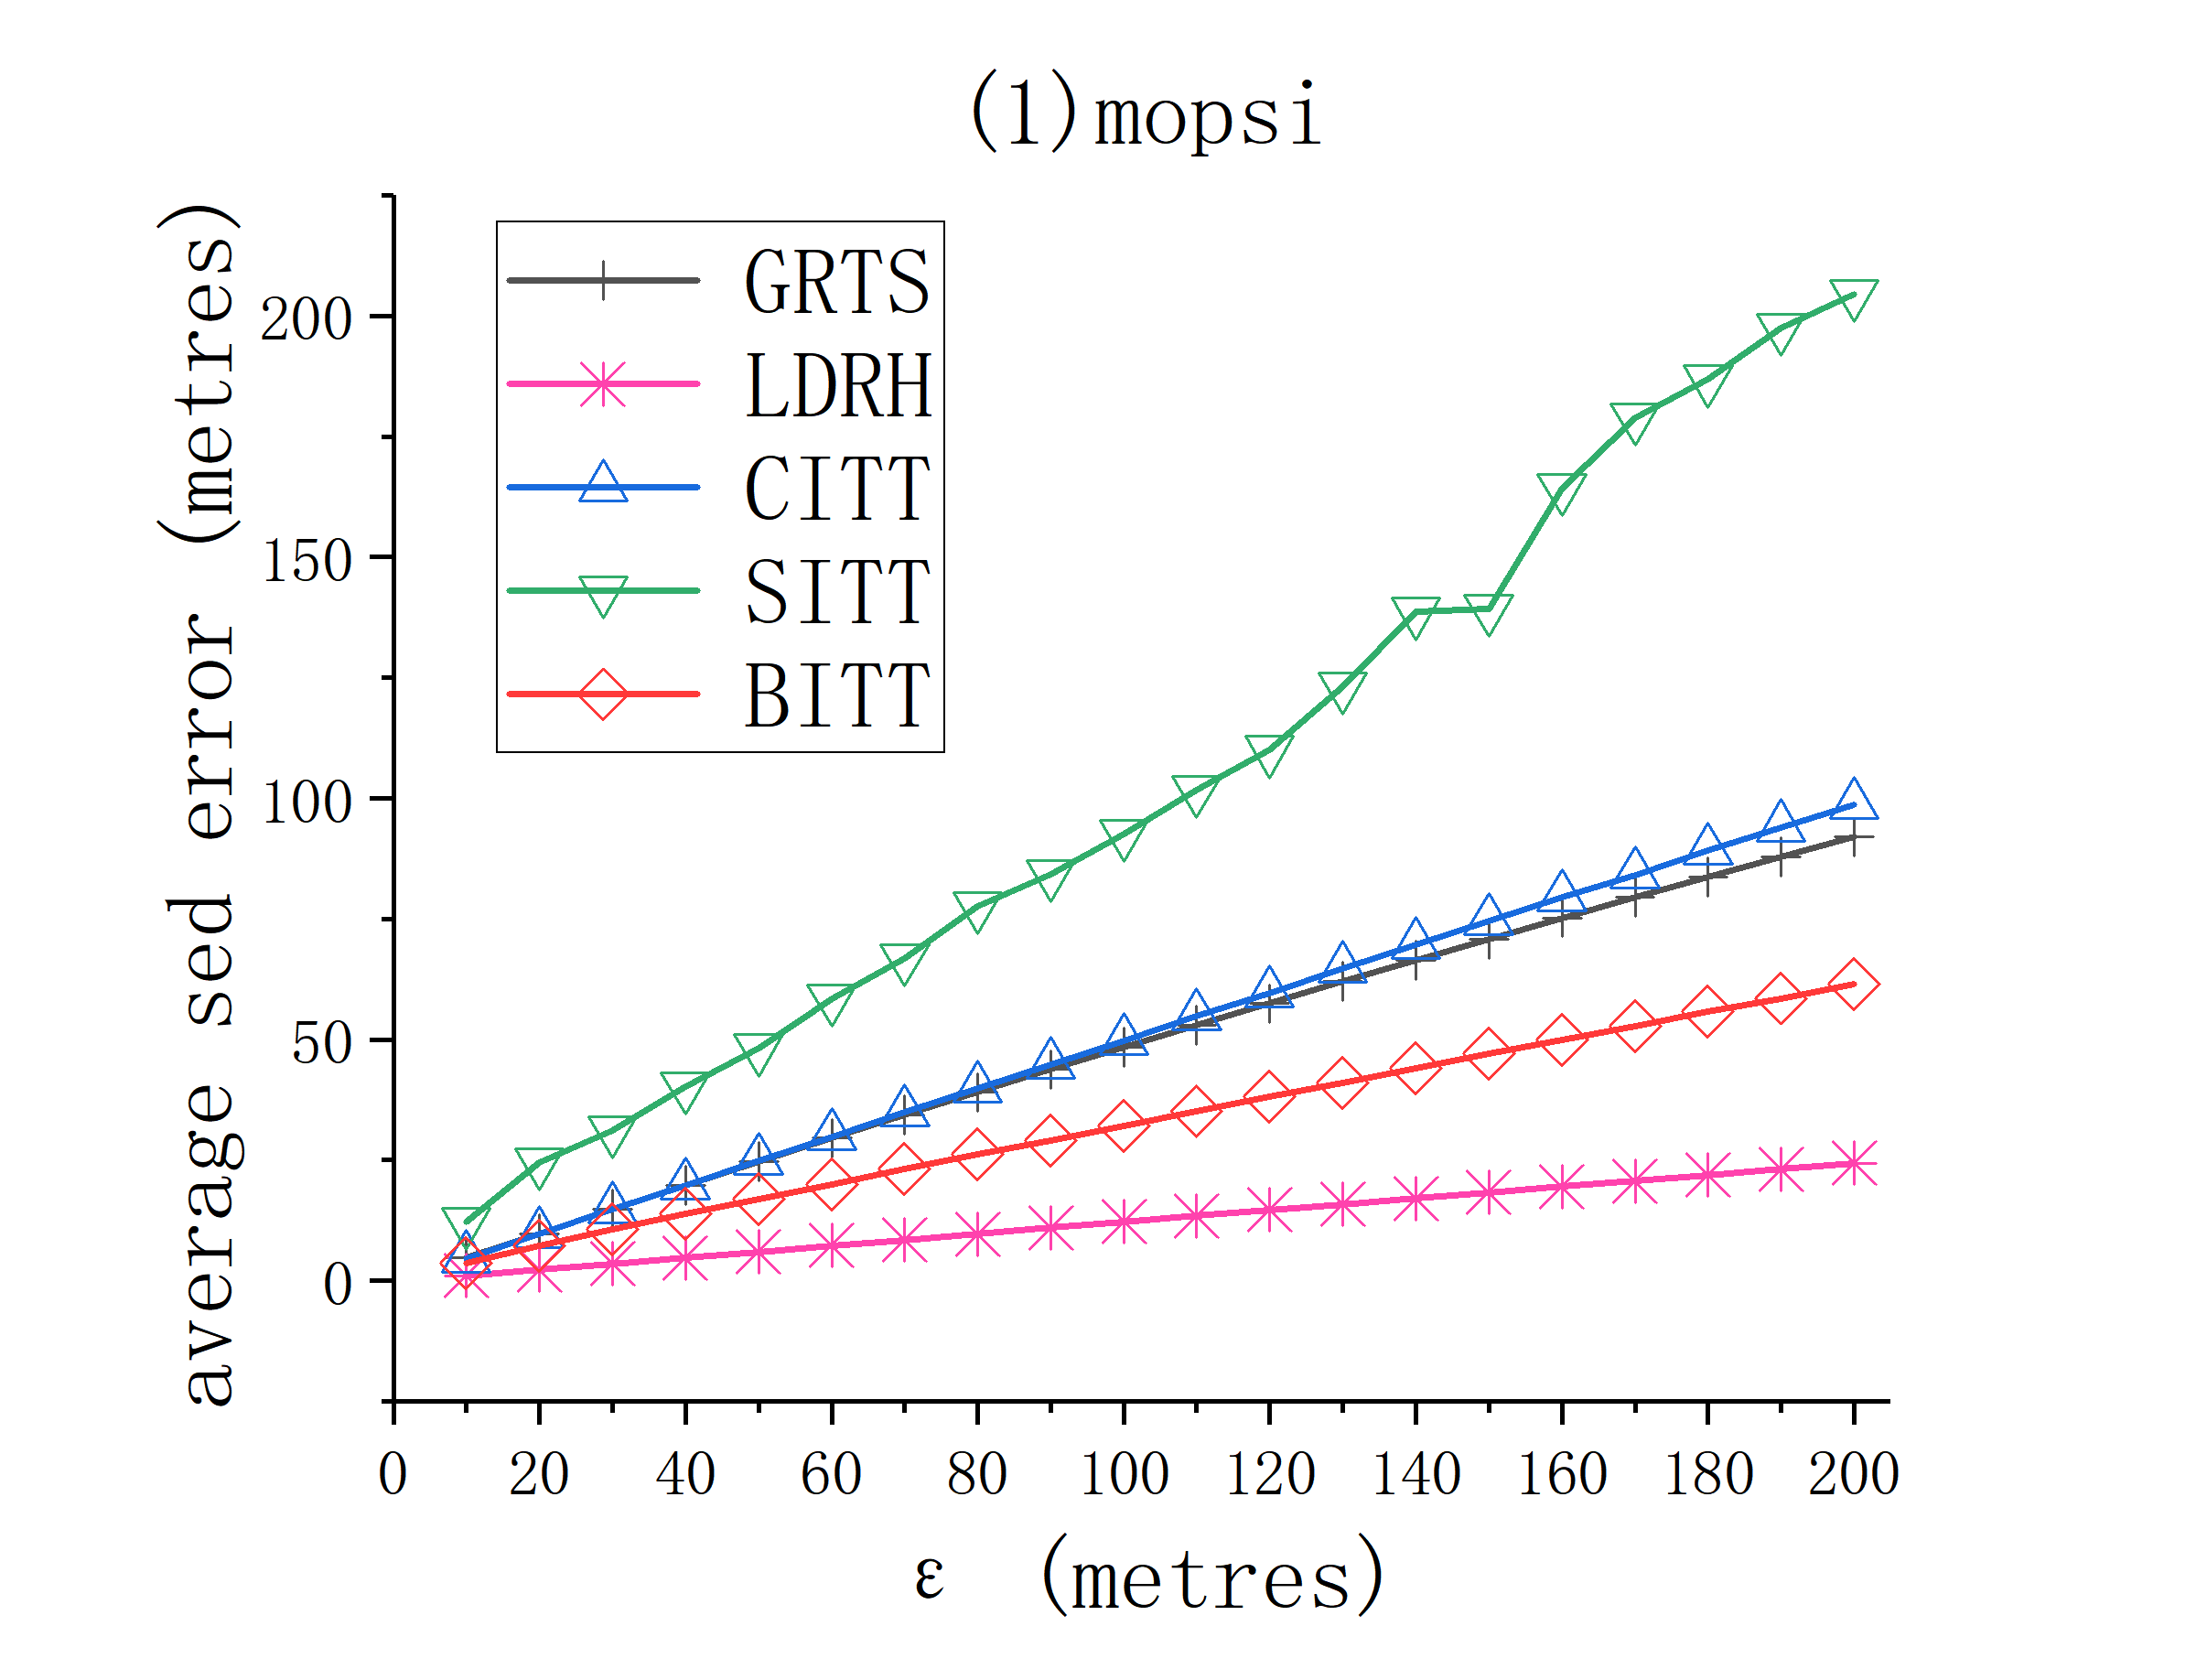
\includegraphics[scale = 0.580]{figures/Fig-mopsi-sed-error.png}\hspace{-1ex}
	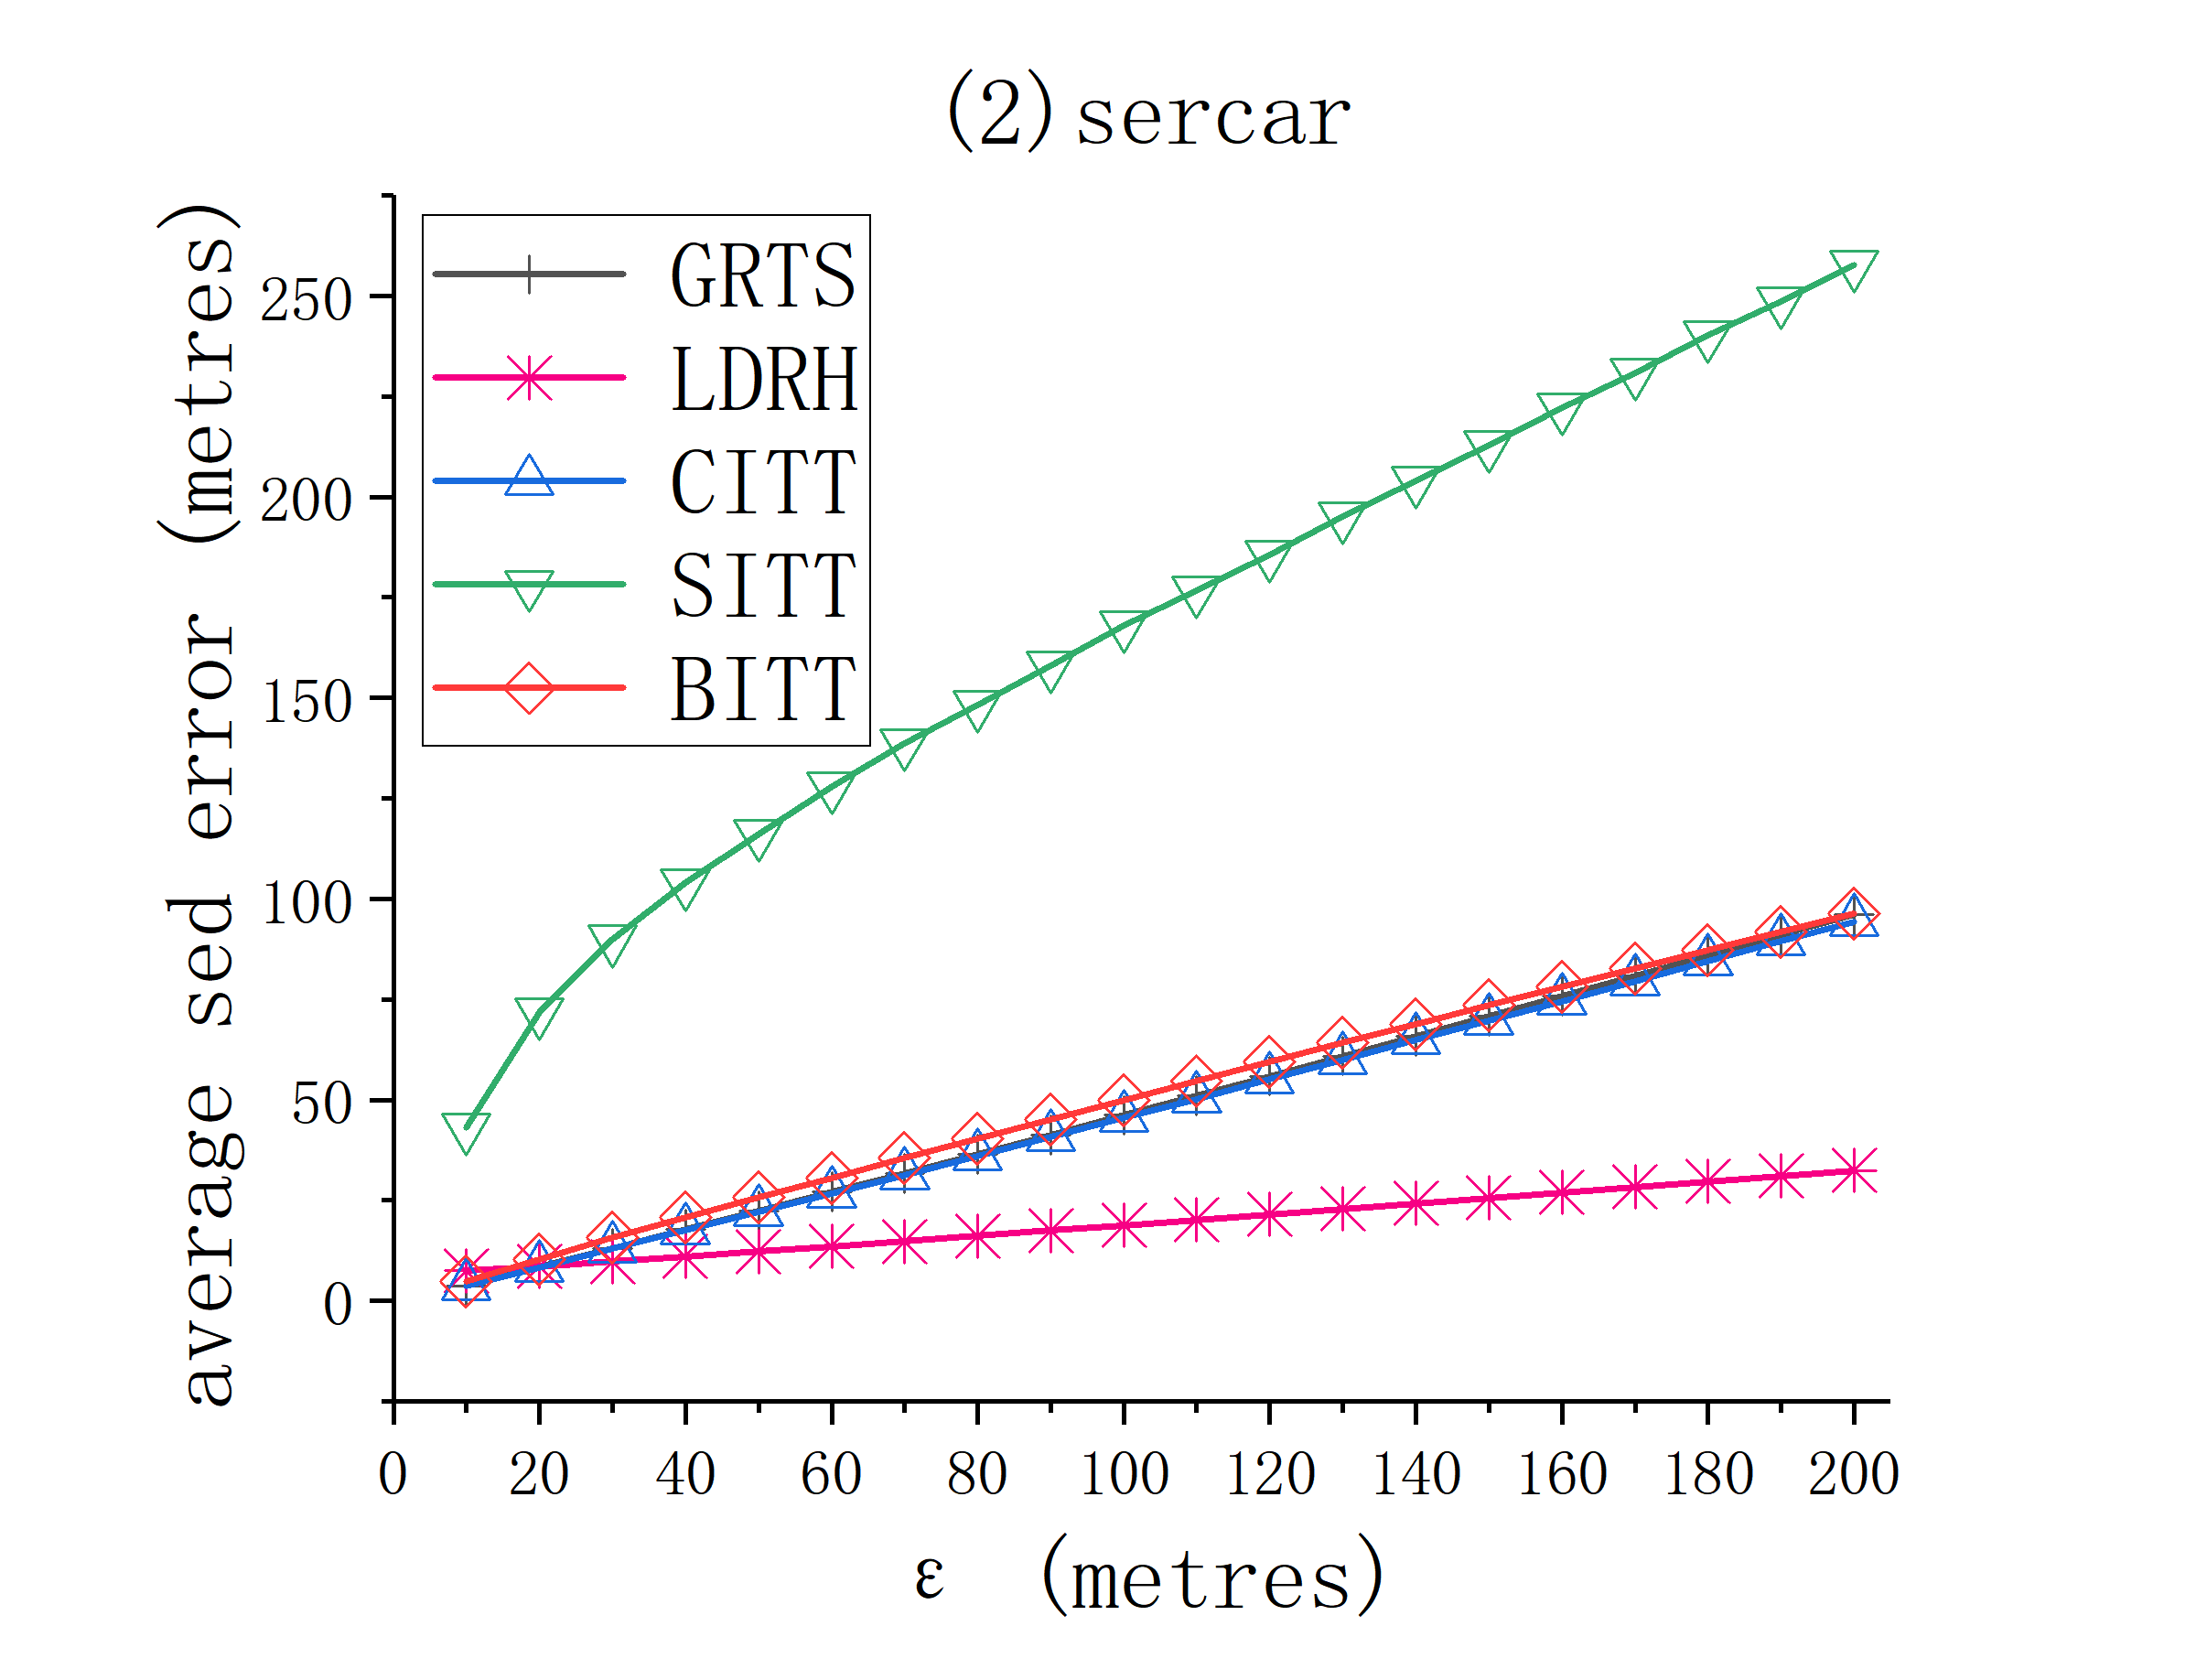
\includegraphics[scale = 0.580]{figures/Fig-sercar-sed-error.png}\hspace{-1ex}
	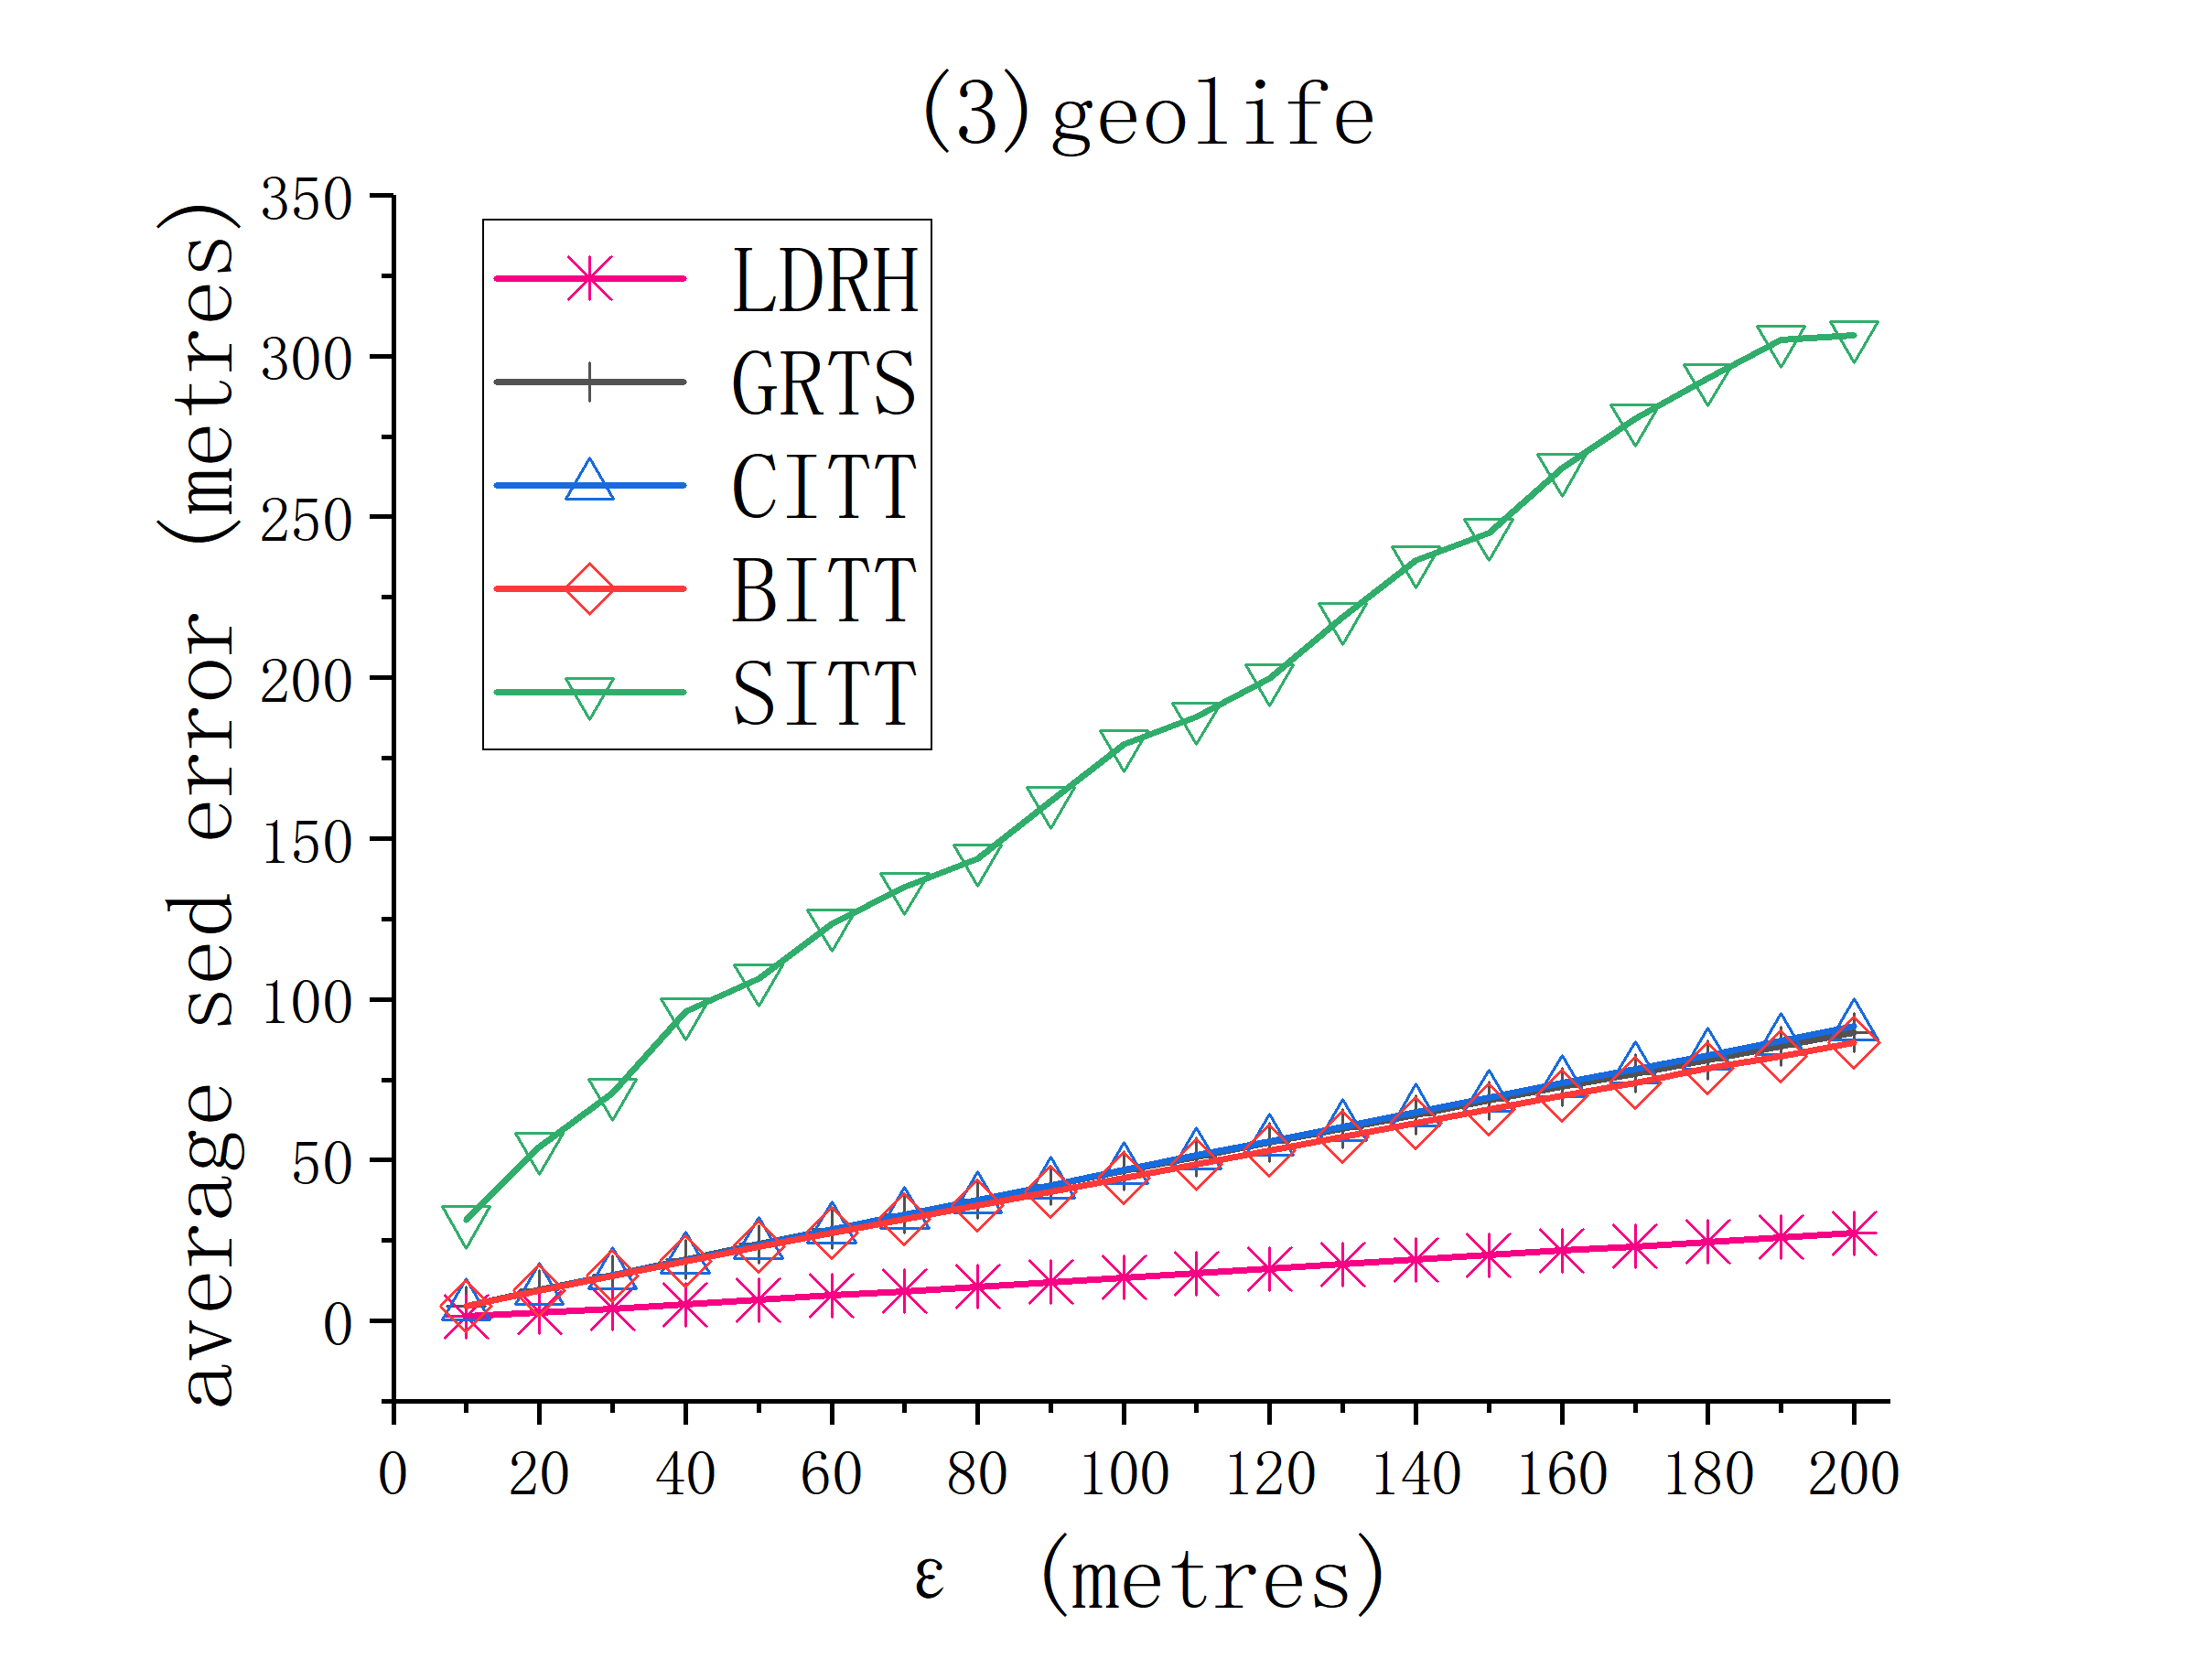
\includegraphics[scale = 0.580]{figures/Fig-geolife-sed-error.png}\hspace{0ex}
	\vspace{-1ex}
	\caption{\small Evaluation of \sed errors: varying error bounds $\epsilon_{sed}$ and $\epsilon_{ped}$.}
	\label{fig:sed-error}
	\vspace{-1ex}
\end{figure*}

\begin{figure*}[tb!]
	\centering
	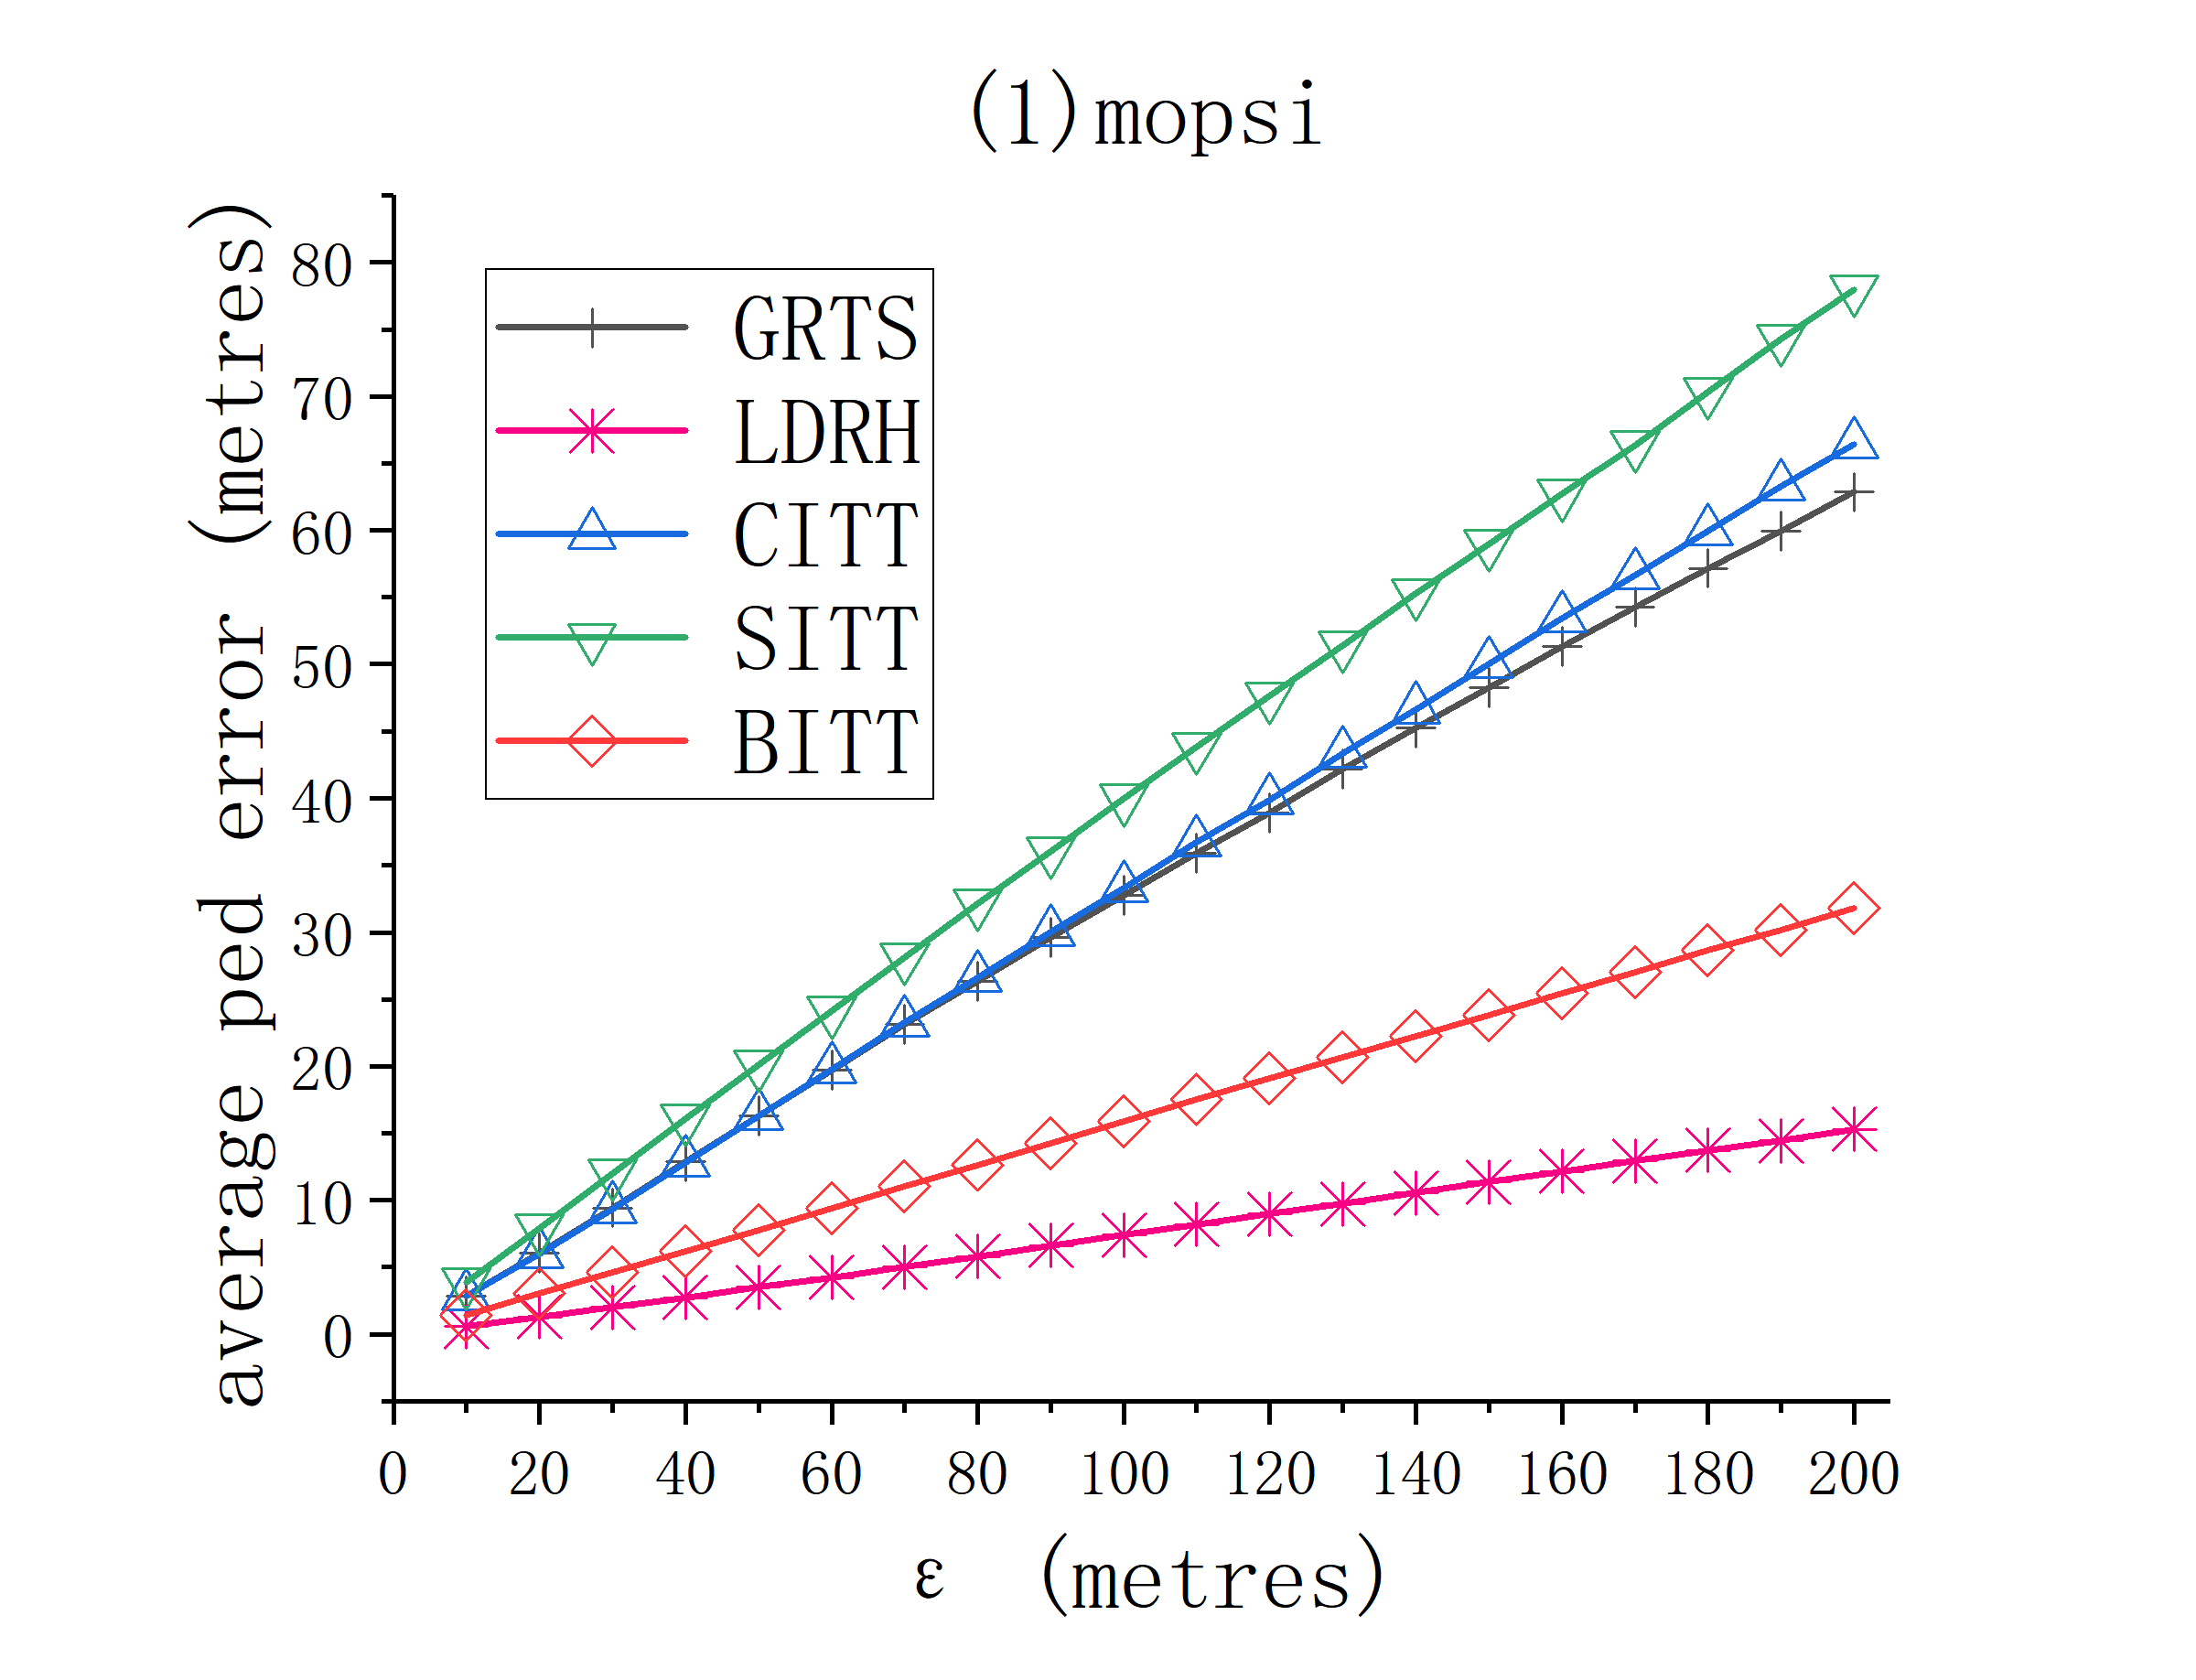
\includegraphics[scale = 0.580]{figures/Fig-mopsi-ped-error.png}\hspace{-1ex}
	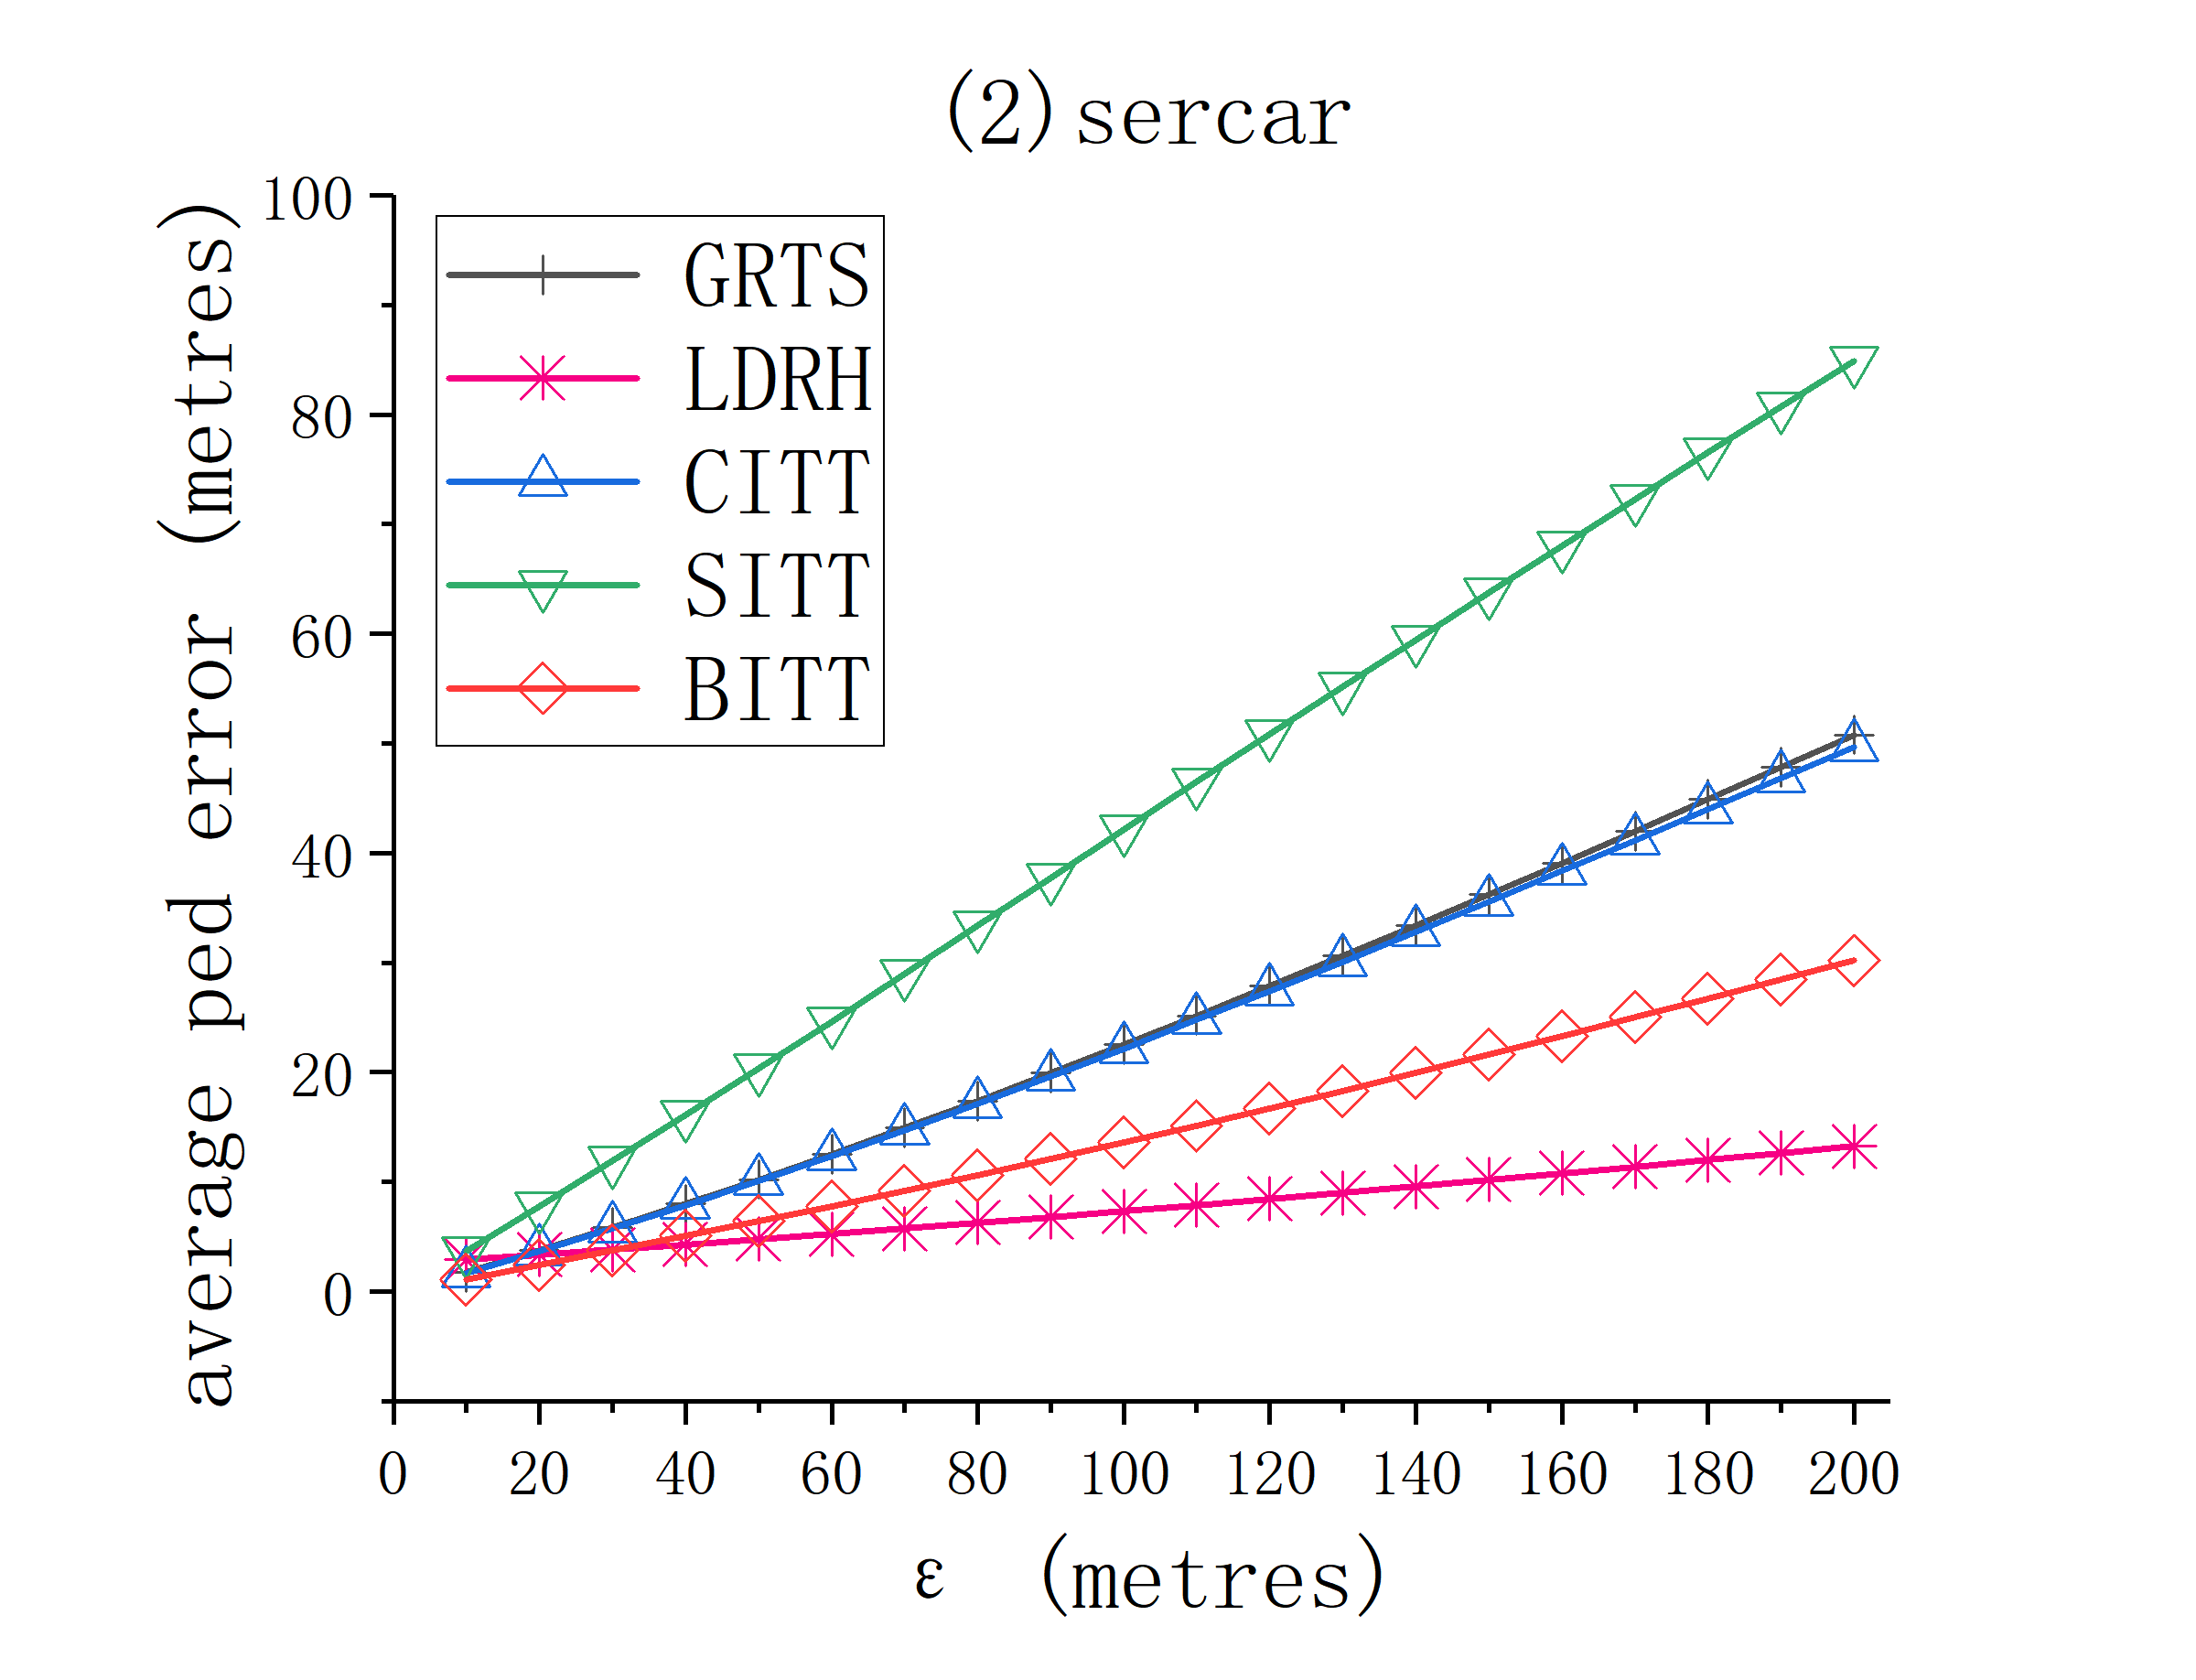
\includegraphics[scale = 0.580]{figures/Fig-sercar-ped-error.png}\hspace{-1ex}
	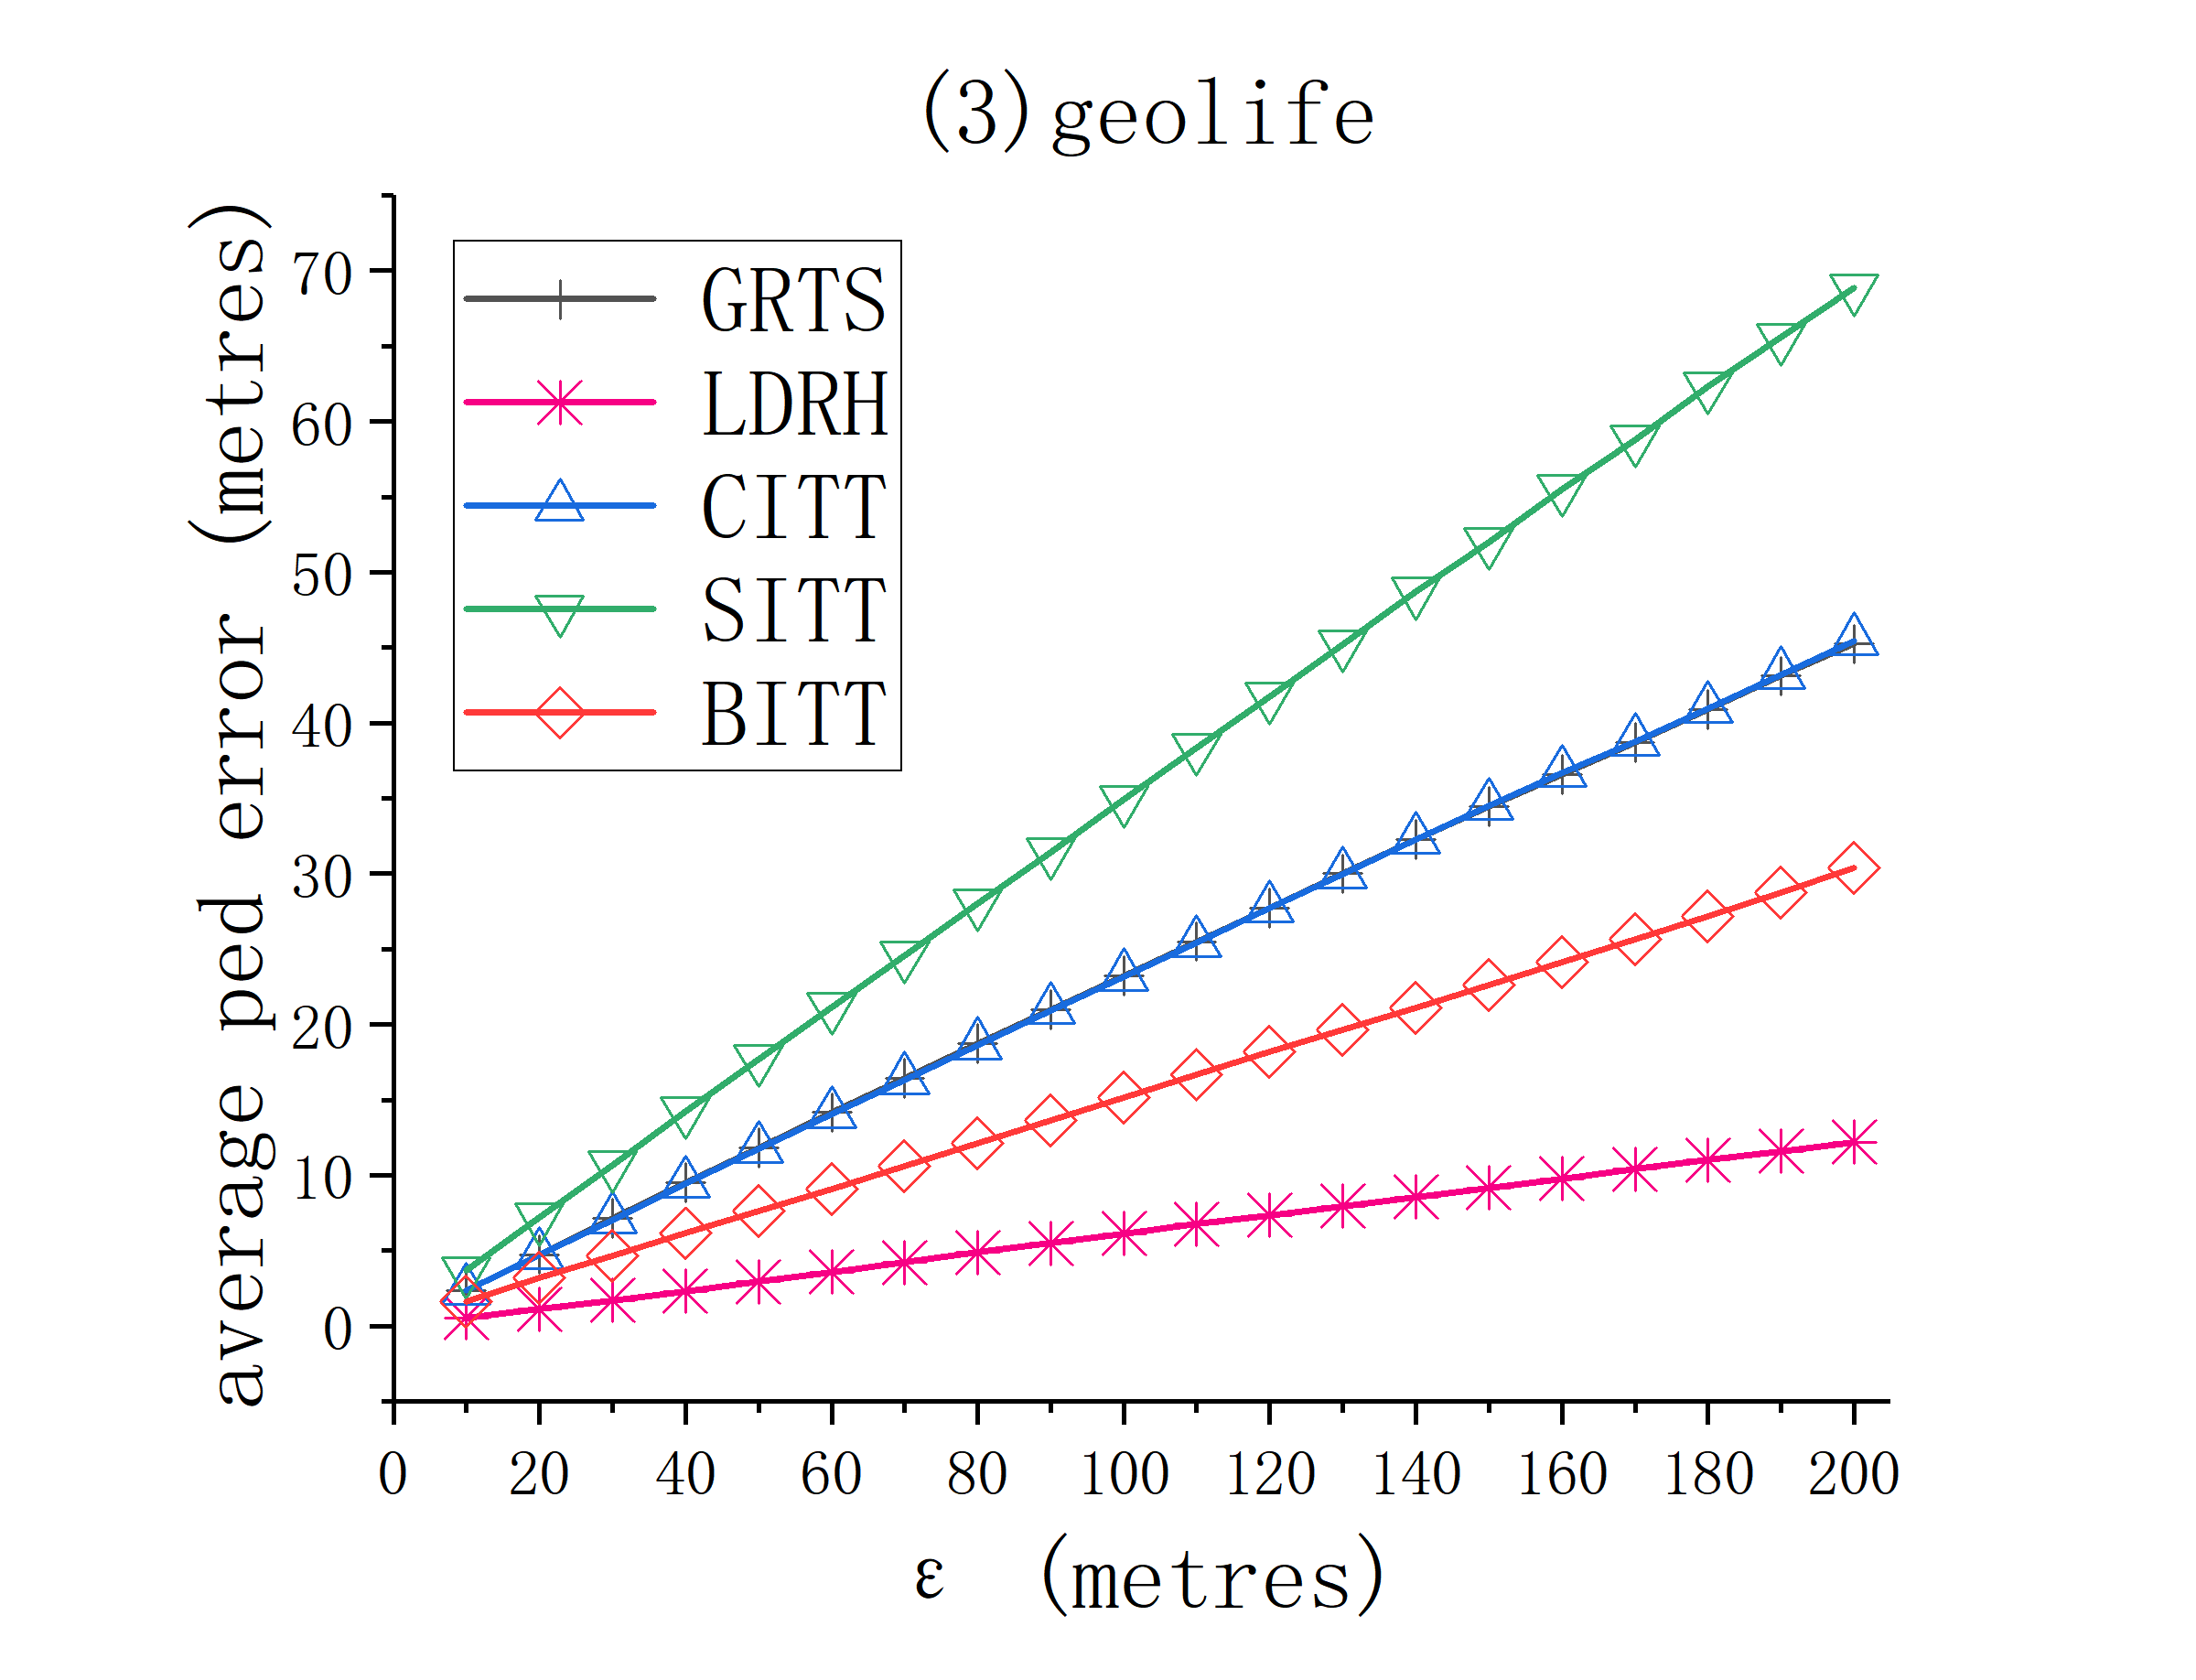
\includegraphics[scale = 0.580]{figures/Fig-geolife-ped-error.png}\hspace{0ex}
	\vspace{-1ex}
	\caption{\small Evaluation of \ped errors: varying error bounds $\epsilon_{sed}$ and $\epsilon_{ped}$.}
	\label{fig:ped-error}
	\vspace{-1ex}
\end{figure*}

\begin{figure*}[tb!]
	\centering
	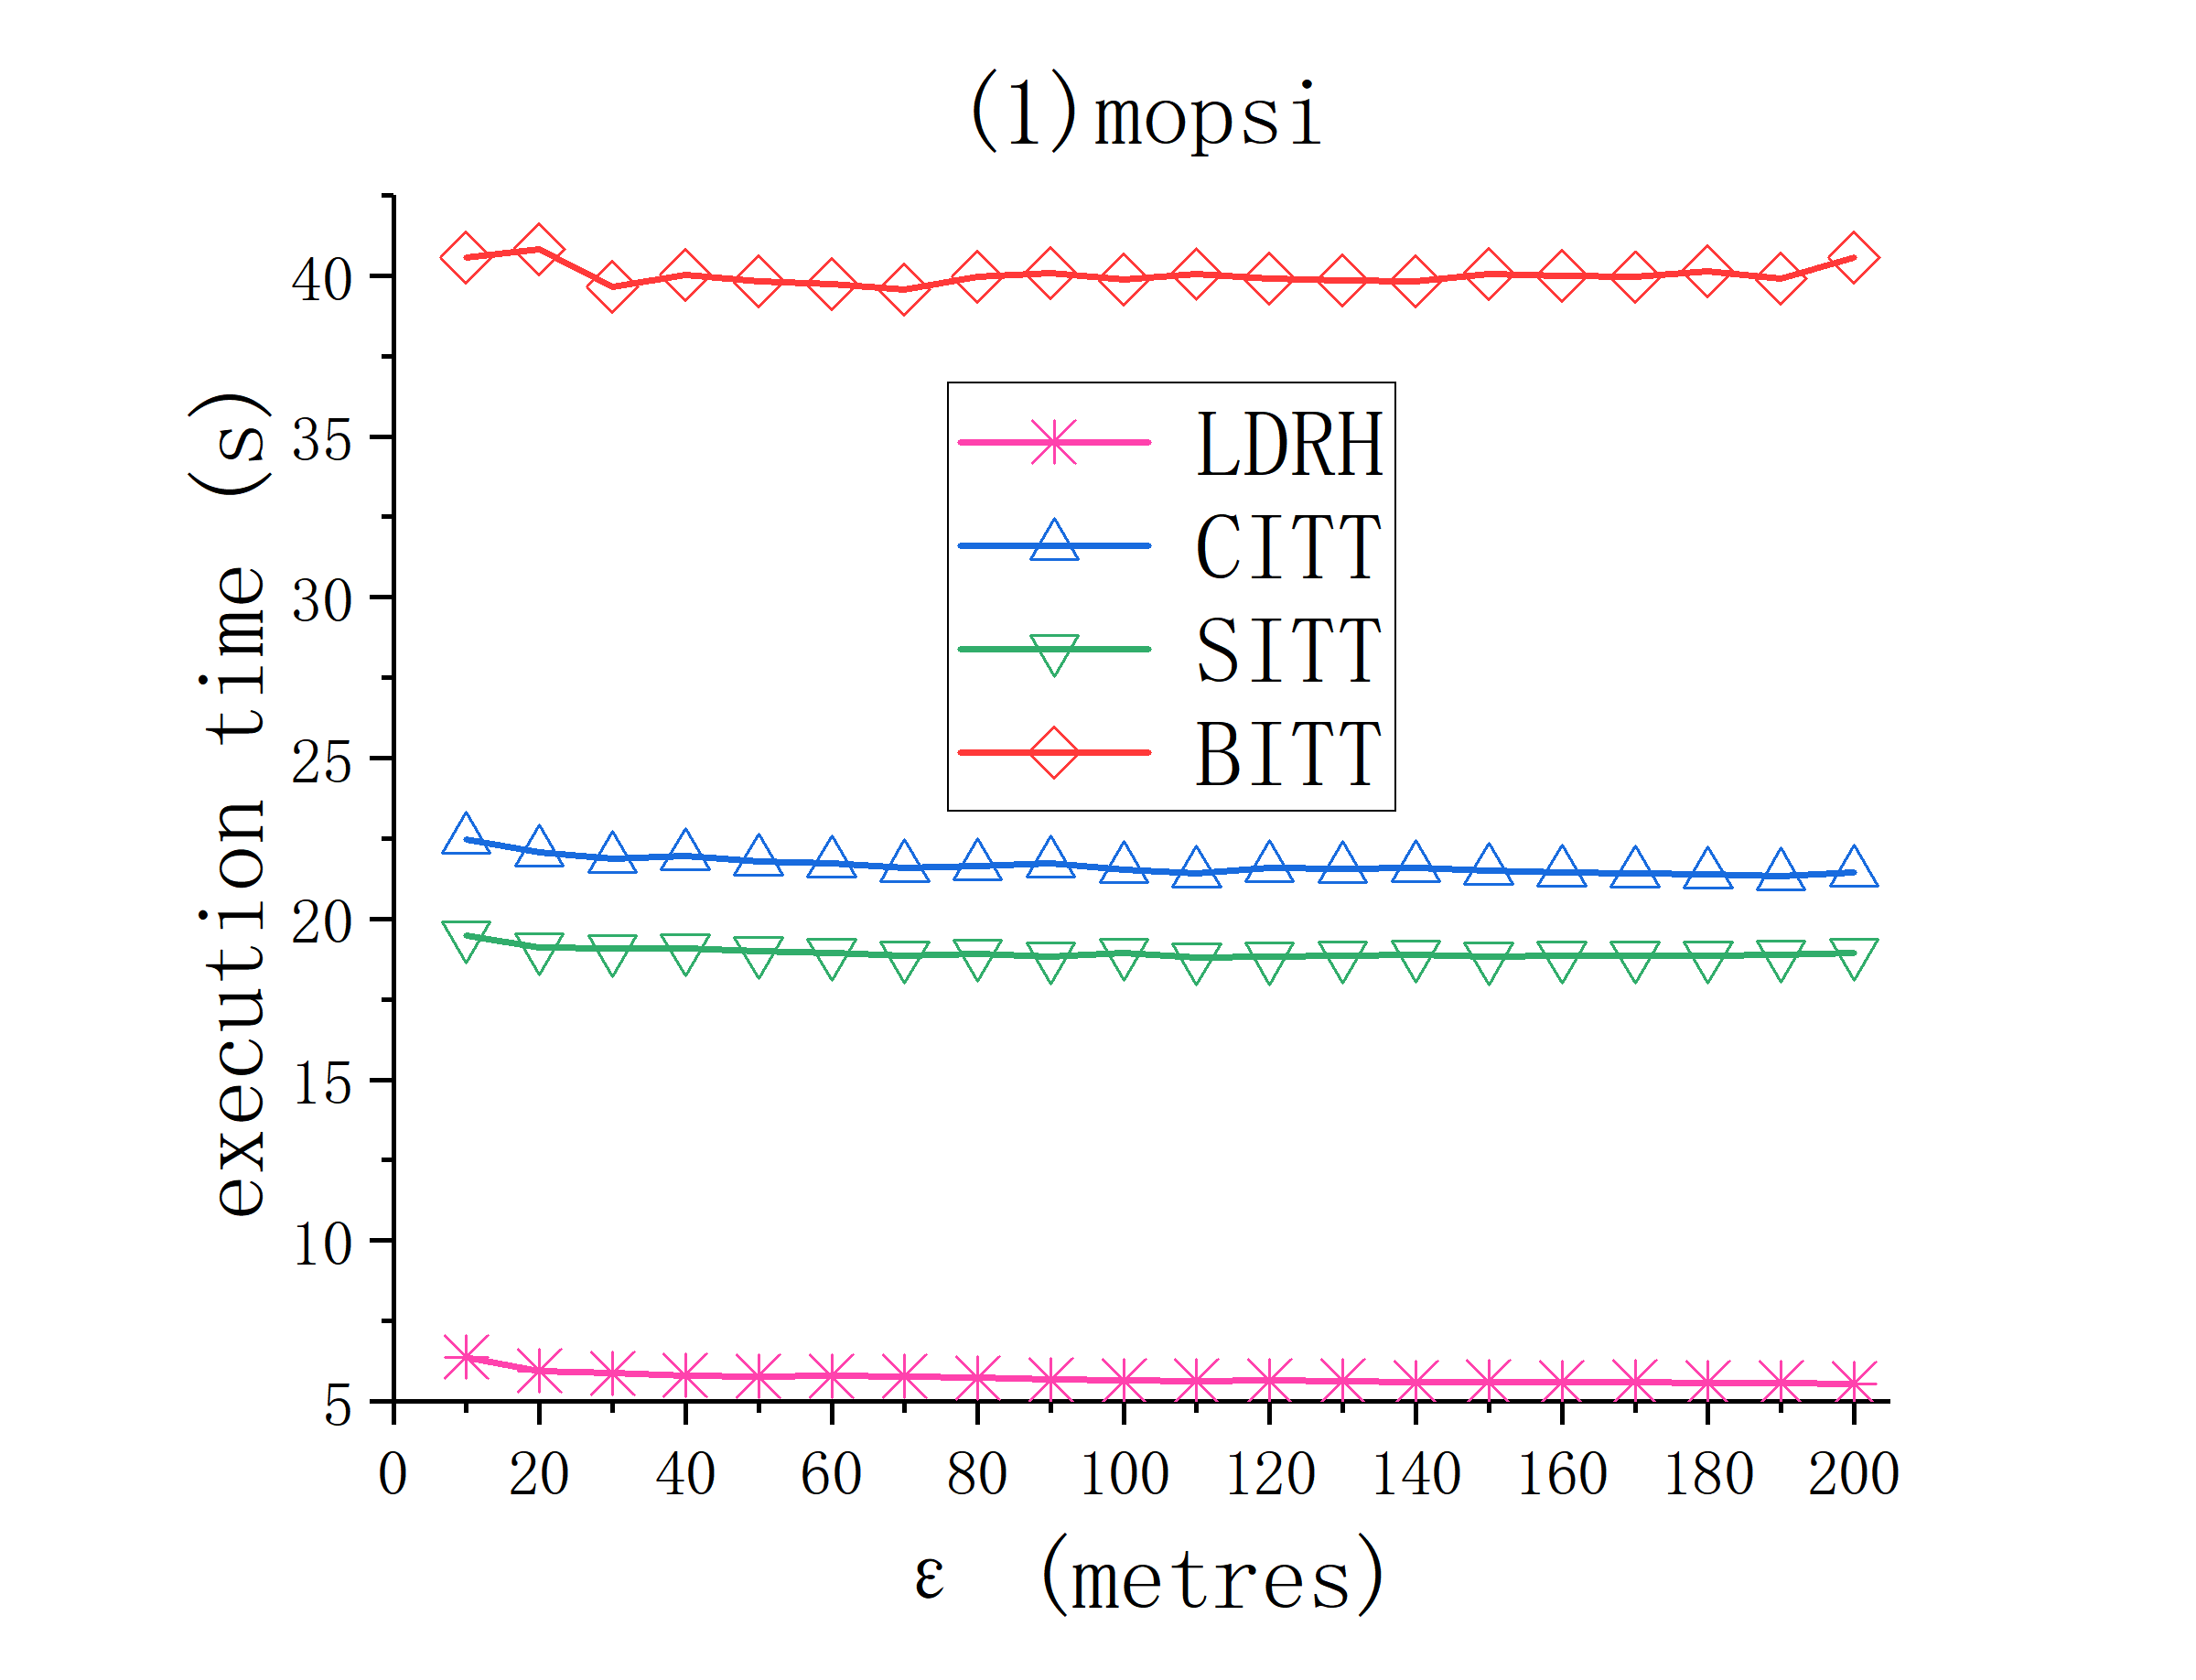
\includegraphics[scale = 0.580]{figures/Fig-mopsi-running-time.png}\hspace{-1ex}
	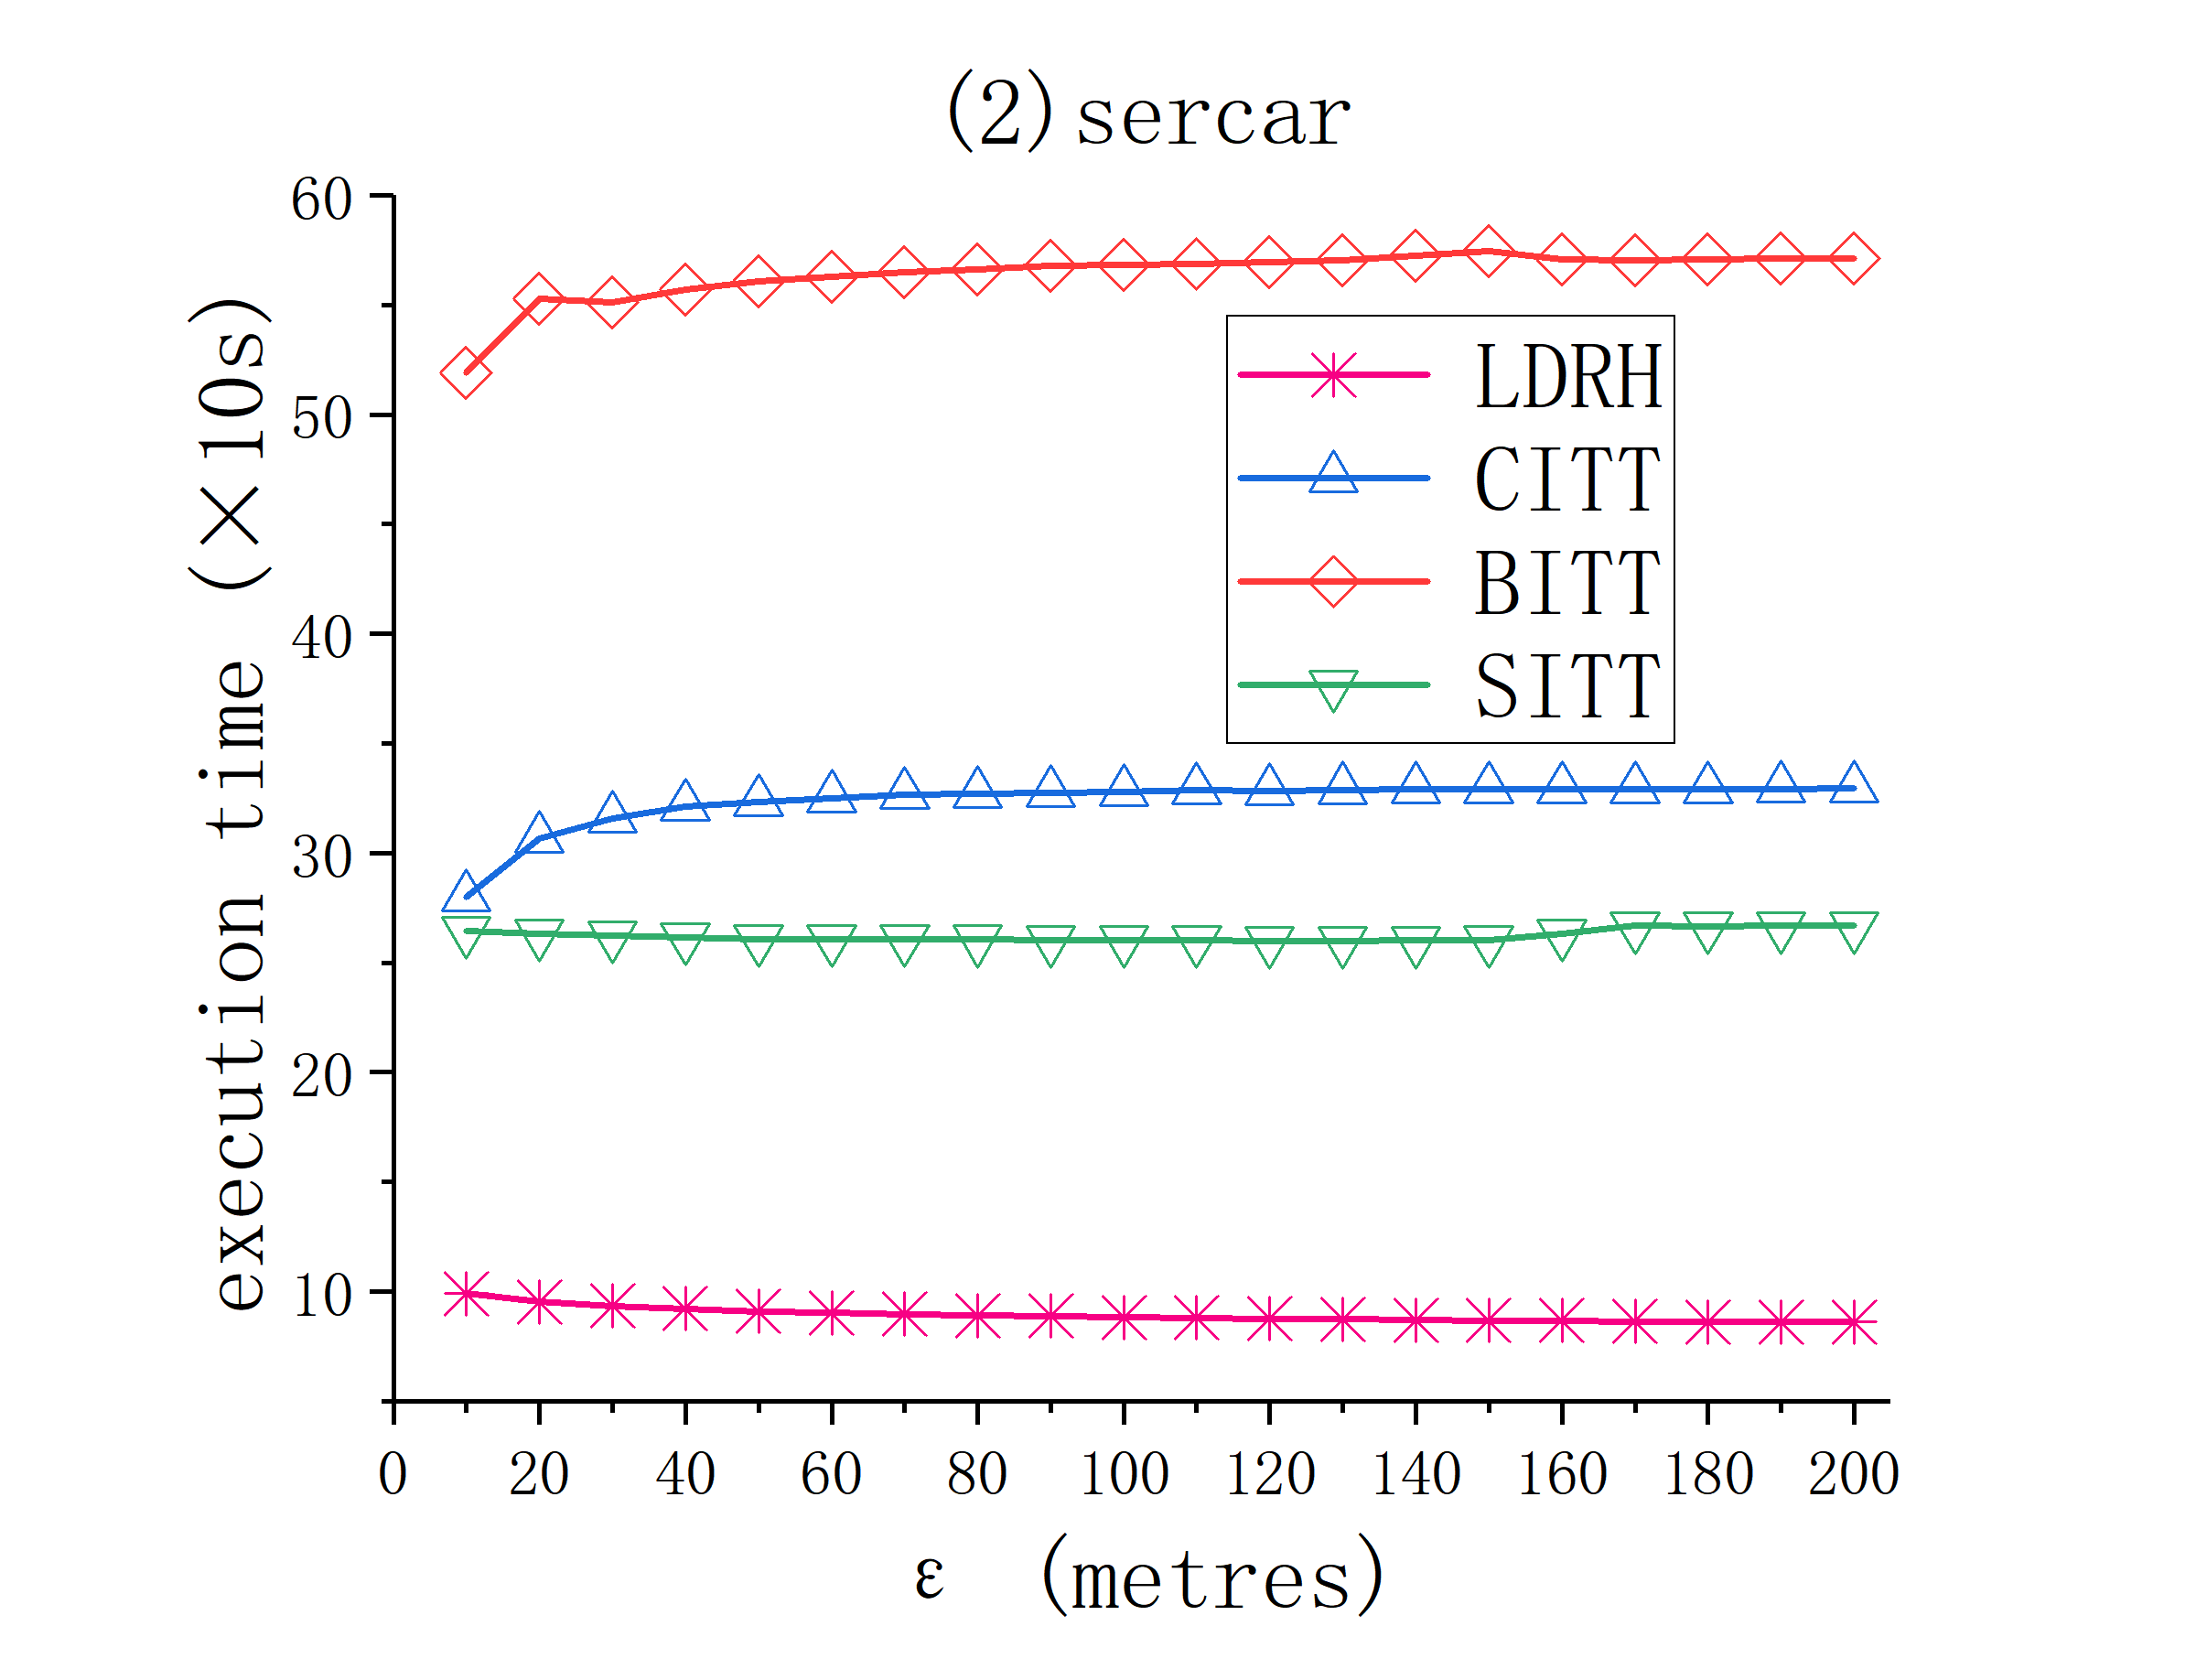
\includegraphics[scale = 0.580]{figures/Fig-sercar-running-time.png}\hspace{-1ex}
	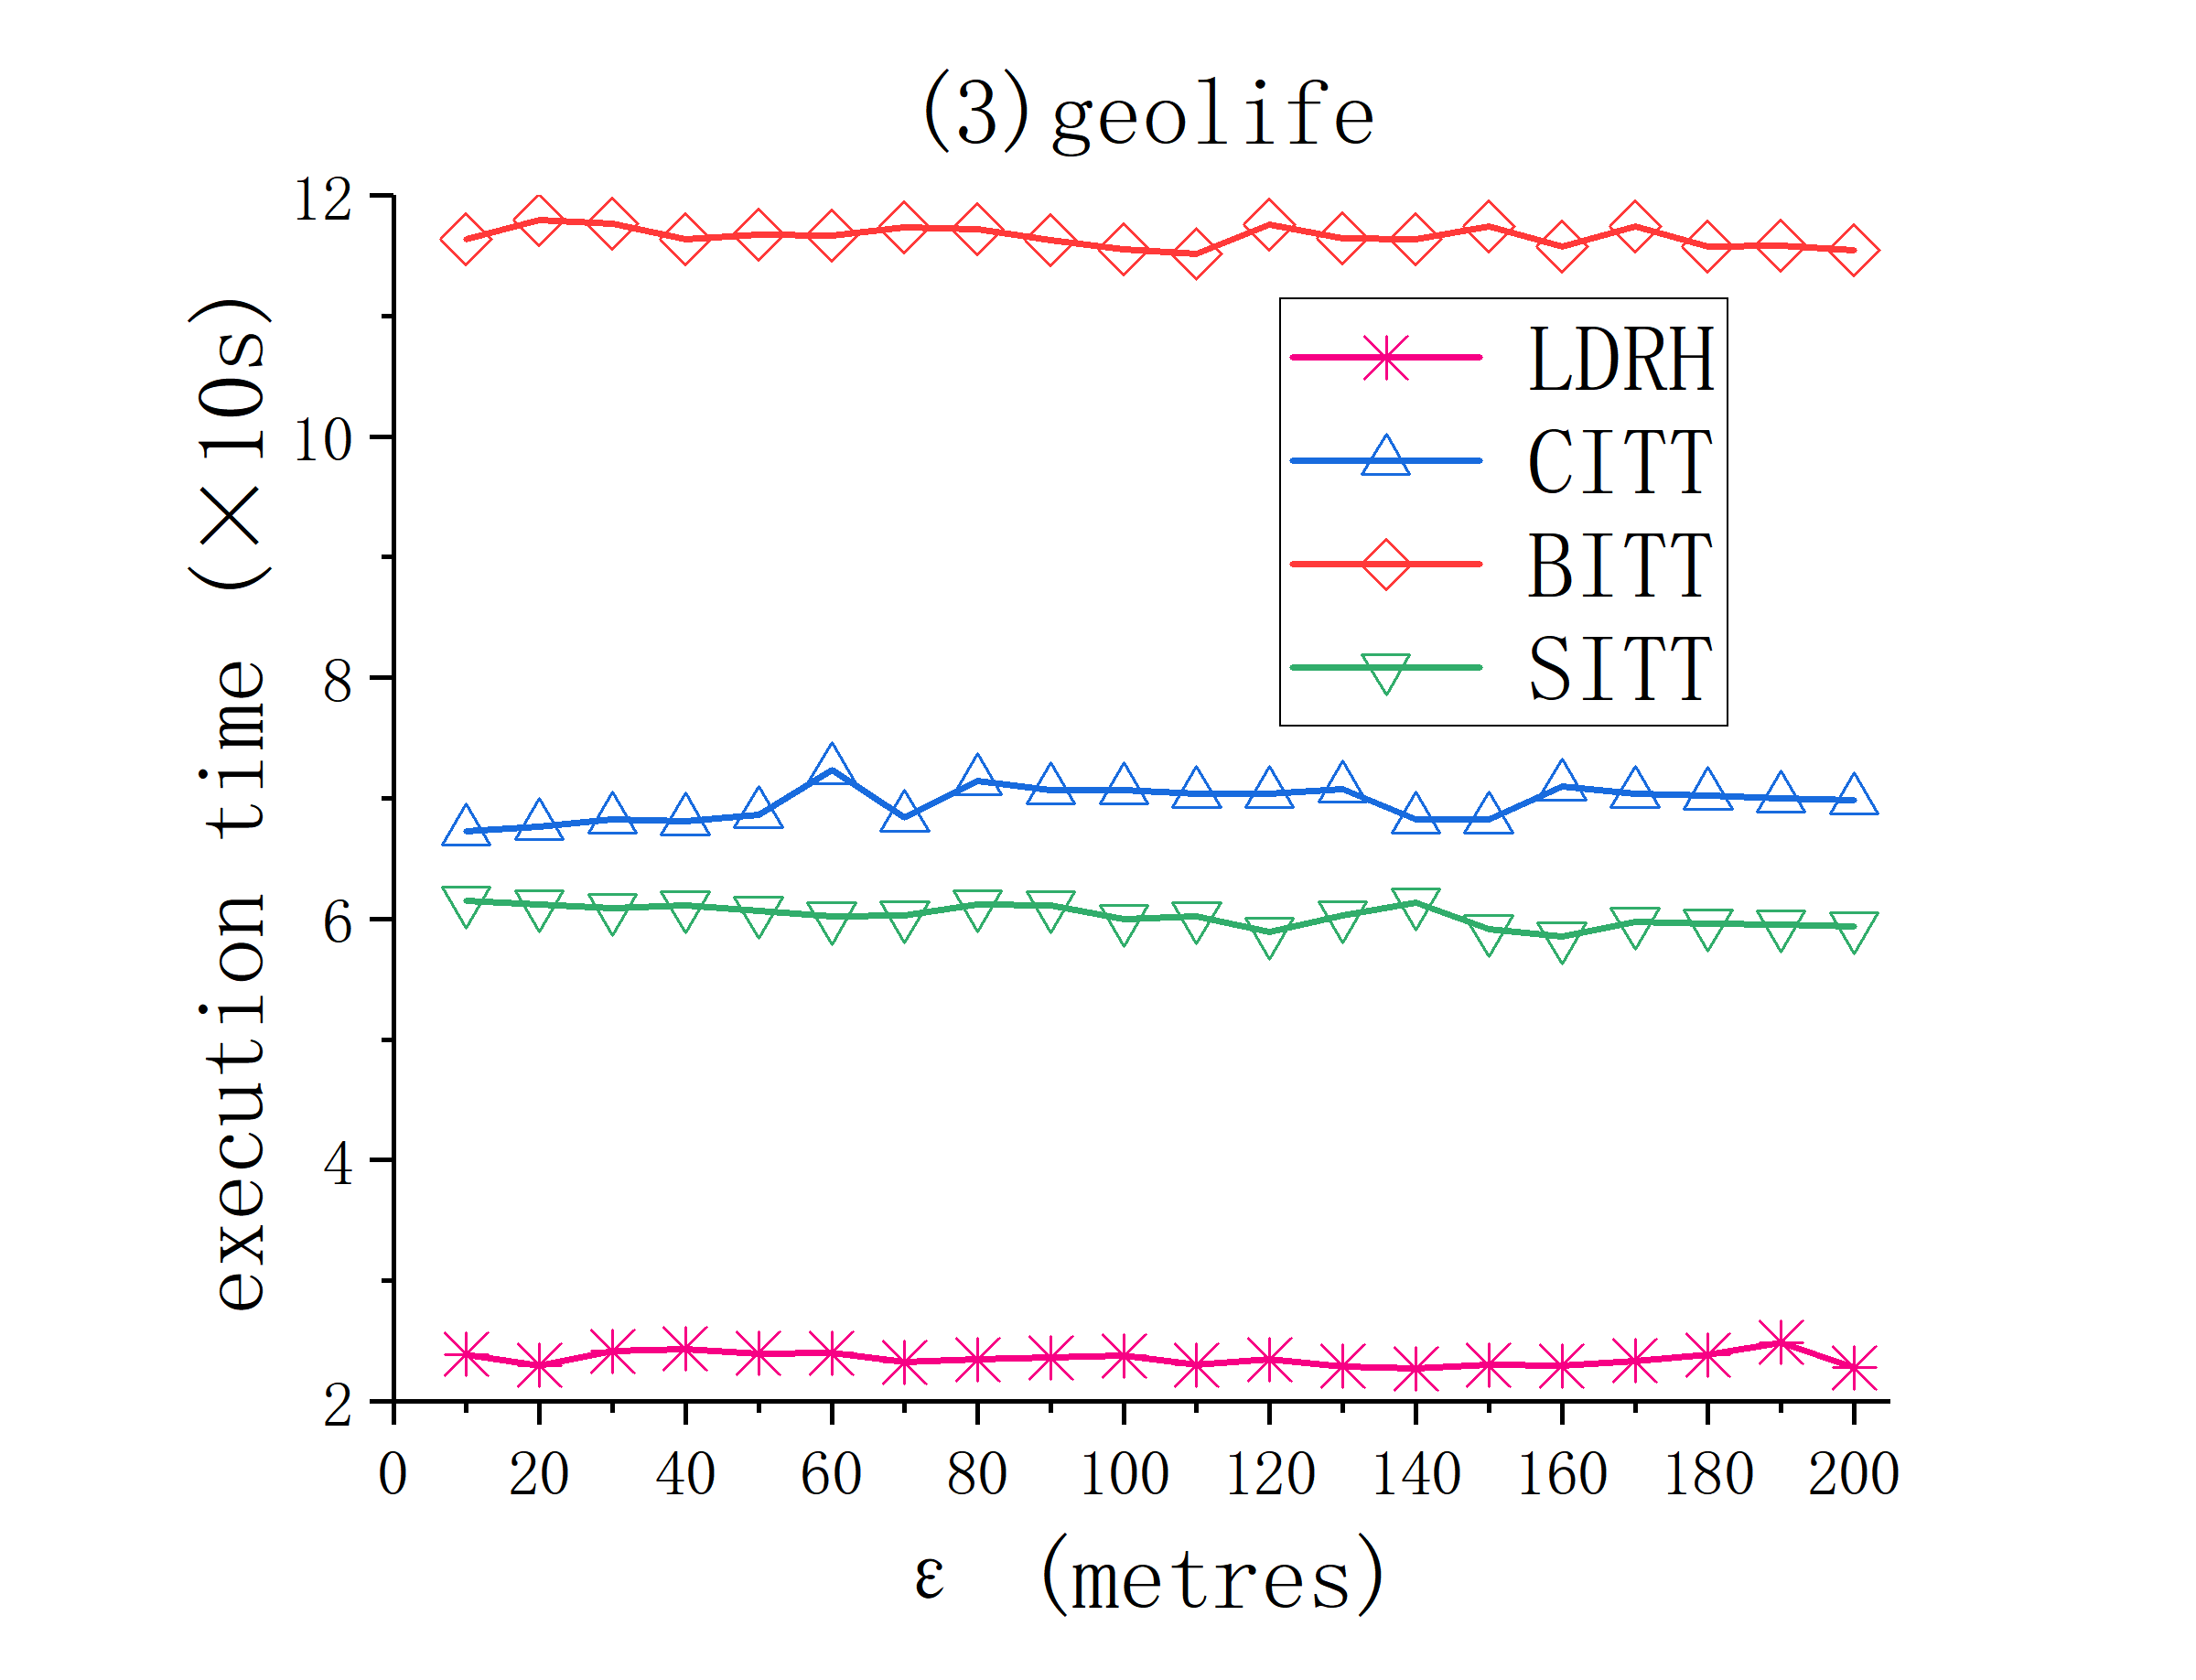
\includegraphics[scale = 0.580]{figures/Fig-geolife-running-time.png}\hspace{0ex}
	\vspace{-1ex}
	\caption{\small Evaluation of running time: varying error bounds $\epsilon_{sed}$ and $\epsilon_{ped}$.}
	\label{fig:running-time}
	\vspace{-1ex}
\end{figure*}


\subsubsection{Comparing algorithms \bitt, \sitt and \citt with \ldrh and \grts.}
This section compares our algorithms \citt, \sitt and \bitt with algorithms \ldrh and \grts.
We varied the error bound (either $\epsilon_{sed}$ or $\epsilon_{ped}$) of \citt, \sitt, \ldrh and \grts from $10$ meters to $200$ meters on the entire three datasets, respectively. 
{For \bitt, its performance depends on the shape of the finite beam, \ie given the same area, it varies \wrt the ratio between $\epsilon_{ped}$ and $\epsilon_{sed}$. {Without losing generality}, we set its $\epsilon_{ped}$ to {$0.5$} times the $\epsilon_{ped}$ of \sitt and its $\epsilon_{sed}$ to {$1.6$} times the $\epsilon_{sed}$ of \citt, \grts and \ldrh, such that the area of the finite beam of \bitt is $3.147\times\epsilon_{sed}^2$, which is approximate to $3.142\times\epsilon_{sed}^2$, the area of the circular of algorithms \citt, \ldrh and \grts~\wrt the given $\epsilon_{sed}$.}
%
The results are reported in Figures~\ref{fig:compression-ratio}, \ref{fig:total-message}, \ref{fig:sed-error}, \ref{fig:ped-error} and \ref{fig:running-time}.


\stitle{Compression ratios.} We first report and analyze the compression ratios from Figure~\ref{fig:compression-ratio}.

\ni (1) When increasing $\epsilon_{sed}$ and $\epsilon_{ped}$, the compression ratios of all these algorithms decrease on all datasets.

\ni (2) \sitt has the best compression ratios, \ldrh is the worst, and \grts, \citt and \bitt are comparable on all datasets and for all $\epsilon$.
The compression ratios of \grts, \bitt,  \citt and \sitt are on average {($27.5\%$, $38.6\%$, $32.2\%$), ($34.9\%$, $37.3\%$, $36.7\%$), ($27.7\%$, $38.9\%$, $32.8\%$) and ($20.2\%$, $19.6\%$, $19.4\%$)} of \ldrh on datasets (\mopsi, \sercar, \geolife), respectively.
For example, when $\epsilon = 40$ meters, \ie~$\epsilon_{sed} = 40$ meters for \ldrh, \grts and \citt, $\epsilon_{ped} = 40$ meters for \sitt and {$(\epsilon_{ped}, \epsilon_{sed}) = (0.5\times 40, 1.6\times 40)=(20, 64)$} meters for \bitt, the compression ratios of \ldrh, \grts, \bitt, \citt and \sitt are
{($10.9\%$, $33.7\%$, $13.6\%$), ($3.0\%$, $13.3\%$, $4.5\%$), {($3.7\%$, $12.7\%$, $5.0\%$)}, ($3.0\%$, $13.2\%$, $4.4\%$) and ($2.1\%$, $6.1\%$, $2.6\%$)} on  {datasets (\mopsi, \sercar, \geolife)}, respectively. 

\ni (3) Datasets have impacts on compression ratios, \ie~datasets with higher sampling rates usually have better performance in terms of compression ratio.
	


\stitle{Message ratios.} We then report and and analyze the message ratios from Figure~\ref{fig:total-message}.

%To evaluate the impacts of distance metrics and error bounds on messages of \citt, \sitt and \bitt vs. \ldrh and \grts, we varied the error bound (either $\epsilon_{sed}$ or $\epsilon_{ped}$) from $10$ meters to $200$ meters on the entire three datasets, respectively. 

\ni (1) When increasing $\epsilon_{sed}$ and $\epsilon_{ped}$, the number of messages of all these algorithms decrease on all datasets.

\ni (2) The message numbers from the largest to the smallest are \ldrh, \grts, \citt, \bitt and \sitt. Among them, \ldrh has the largest messages because it has the worst compression ratios (thus it produces many \emph{position-velocity-messages}), and \sitt has the least messages because it has the best compression ratios (corresponding to the least \emph{position-velocity-messages}) and at the same time it seldom updates velocities during the process of a sub-trajectory (thus it only sends a small amount of \emph{velocity-messages}).

%(all of them are \emph{position-velocity-messages})
%\ni (2) Since \ldrh updates the position information every time the velocity is updated, the percentage of \emph{velocity-messages} is always $50\%$ of all messages.

\ni (3) \citt has a medium amount of messages (including \emph{position-velocity-messages} and \emph{velocity-messages}) and \bitt is between \citt and \sitt in this test.


\ni (4) \grts has more messages than \citt. Recall that \grts has \emph{position-messages} and \emph{position-velocity-messages}, while \citt has \emph{velocity-messages} and \emph{position-velocity-messages}. From Figure \ref{fig:compression-ratio} we know that \grts has a similar compression ratio as \citt, meaning \grts has the similar number of \emph{position-messages} as the \emph{position-velocity-messages} of \citt. Besides, the  number of \emph{position-velocity-messages} of \grts ({on average $(61.81\%, 59.28\%, 61.85\%)$} of the total messages \wrt datasets (\mopsi, \sercar, \geolife), respectively) is usually a bit larger than the \emph{velocity-messages} of \citt (on average $(60.41\%, 57.31\%, 52.80\%)$ of the total messages \wrt datasets (\mopsi, \sercar, \geolife), respectively). As a result, \grts has more total messages than \citt.

%This is because \grts only updates the velocities messages when the buffer is cleared, and mainly transmits position information.




\stitle{Errors.} We next report and analyze the maximal and average errors from Table~\ref{tab:max-error} and Figures~\ref{fig:sed-error} and \ref{fig:ped-error}.

%The results are reported in Figures~\ref{fig:sed-error} and Figure~\ref{fig:ped-error}.

\ni (1) The maximal \ped and \sed errors of these algorithms are not larger than the error bounds we set in these tests, except the maximal \sed error of \sitt, as \sitt is bounded by \ped, not by \sed. These tests also confirm that if an algorithm is bounded by a \sed threshold, then it must be bounded by \ped with the same threshold.

\ni (2) The average errors increase with the increase of $\epsilon_{sed}$ and $\epsilon_{ped}$.

\ni (3) The average \sed errors of these algorithms from the largest to the smallest are \sitt, \citt (also \grts and \bitt) and \ldrh. The average \sed errors of algorithms \grts, \citt \bitt and \sitt are on average
($400.6\%$, $226.3\%$, $348.6\%$), ($412.7\%$, $222.8\%$, $350.1\%$), ($307.9\%$, $242.6\%$, $336.3\%$) and ($842.0\%$, $857.5\%$, $1452.5\%$)
of \ldrh on datasets (\mopsi, \sercar, \geolife), respectively.

\ni (4) The average \sed errors of \bitt are equal to or less than compression effective algorithms \grts and \citt, through it actually uses a larger \sed error bound, \ie~1.6 times of \sed threshold of \grts and \citt in these tests.

\ni (5) The average \ped errors of these algorithms from the largest to the smallest are \sitt, \grts (also \citt), \bitt and \ldrh. Among them, the average \ped errors of \citt is very close to \grts. The average \ped errors of algorithms \grts, \citt, \bitt and \sitt are on average
($443.7\%$, $ 283.0\%$, $ 390.2\%$), ($452.2\%$, $278.1\%$, $388.9\%$), ($ 268.2\%$, $ 201.5\%$, $ 256.1\%$)
and ($550.5\%$, $517.0\%$, $589.0\%$)
of \ldrh on datasets (\mopsi, \sercar, \geolife), respectively.

\ni (6) The average \ped errors of \bitt are obviously less than compression effective algorithms \grts, \citt and \sitt, because it actually uses a smaller \ped error bound, \ie~$0.5$ times \ped of \sitt (recall the \ped error bound of \sitt is set to the same value of the \sed error bound of \grts and \citt) in these tests.



\begin{table}[tb!]
	\renewcommand{\arraystretch}{1.20}
	\caption{\small The maximal errors}
	\vspace{-1.5ex}
	\centering
	\footnotesize
	%\scriptsize
	\begin{tabular}{|l|c|c|c|c|c|c|}
		\hline
		\multirow{2}*{\bf{Alg.}\hspace{-1ex}} & \multicolumn{3}{c|}{Max SED error} & \multicolumn{3}{c|}{Max PED error} \\
		\cline{2-7}
		 &\hspace{-1ex}\sercar\hspace{-1ex}&\hspace{-1ex}\geolife&\hspace{-1ex}\mopsi  &\hspace{-1ex}\sercar\hspace{-1ex}&\hspace{-1ex}\geolife&\hspace{-1ex}\mopsi \\
		\hline
		\ldrh\hspace{-1ex}& 56.81 &	59.24 &	57.93 &	56.51 &	57.74 &	56.05 \\
		\hline
		\grts\hspace{-1ex}	&60.00 & 60.00 &	60.00 &	59.99 &	60.00 &	60.00\\
		\hline 
		\citt\hspace{-1ex}	&60.00 &	60.00 &	59.99 &	59.95 &	59.98 &	59.93 \\
		\hline 
		\bitt &	95.94 &	96.00 &	95.98 &	30.00  &	30.00 &	30.00 \\
		\hline
		\sitt\hspace{-1ex} & \hspace{-1ex}$1.40\times 10^6$ & \hspace{-1ex}$5.26\times 10^6$	& \hspace{-1ex}$1.92\times 10^6$ &	60.00 &	60.00 &	60.00 \\
		\hline
		
		
	\end{tabular}
	\label{tab:max-error}
	\vspace{-2ex}
\end{table}


%%%%%%%%%%%%%%%%% running time
%In this part of experiments, we compare the running time of our algorithms \citt, \sitt and \bitt with \ldrh and \grts.
%The results are reported in Figure~\ref{fig:running-time}. 
\stitle{Running time.} We finally report and analyze the running time.
Since the running time of \grts is hundreds of times slower than other algorithms, it is not shown in Figure~\ref{fig:running-time}.

\ni (1) The error bound $\epsilon$ has few impacts on running time of \citt, \sitt, \bitt and \ldrh.

\ni (2) The running time of \bitt is approximately the sum of \citt and \sitt, because it combines the logic of \citt and \sitt.

\ni (3) The running time of these algorithms from the largest to the smallest are \grts, \bitt, \citt, \sitt and \ldrh on all datasets.
The average running time of algorithms \grts, \citt, \bitt and \sitt is on average
($116600.1\%$, $2549.6\%$, $69657.1\%$), ($378.8\%$, $363.2\%$, $296.4\%$), ($702.8\%$, $632.9\%$, $496.1\%$)
and ($331.5\%$, $294.1\%$, $256.4\%$)
of \ldrh on datasets (\mopsi, \sercar, \geolife), respectively.


\subsubsection{Summary.} % and discuss
From these tests we find the followings.

\sstab\emph{(1) Compression ratios}. The optimal \sitt algorithm has the best compression ratios among all the algorithms. Algorithm \bitt and \citt are comparable with \grts.
They are all better than \ldrh.

\sstab\emph{(2) Message ratios}. The message numbers from the largest to the smallest are \ldrh, \grts, \citt, \bitt and \sitt.

\sstab\emph{(3) Average errors}. The average errors of these algorithms from the largest to the smallest are \sitt, \grts, \citt and \ldrh. Among them, the average error of \citt is very close to \grts.

\sstab\emph{(4) Running time}. Algorithm \ldrh is the fastest and \grts is the slowest. Moreover, the running time of \bitt is approximately the sum of \citt and \sitt.

In a conclusion, \ldrh runs the fastest and has the lowest average errors at a price of the poorest compression and message ratio. \sitt outperforms \grts in every metrics except average errors. \citt outperforms \grts in message ratio and running time, and is comparable with \grts in compression ratio and average errors. \bitt is comparable with \citt except that it has smaller average errors and longer running time.